\documentclass[a4paper,12pt]{article}
\usepackage[a4paper,left=3cm,right=2cm,top=2cm,bottom=2cm]{geometry}
\usepackage{iftex}
\ifPDFTeX
\PackageError{IEEE_FULL_PAPER}{This report must be compiled with XeLaTeX}{Run xelatex IEEE_FULL_PAPER.tex from the docs/ directory.}
\fi
\usepackage{fontspec}
\setmainfont{Times New Roman}
\usepackage{unicode-math}
\setmathfont{Cambria Math}
\usepackage{setspace}
\setstretch{1.35}
\AtBeginDocument{\fontsize{13pt}{18.2pt}\selectfont}
\setlength{\parindent}{1.25em}
\usepackage{indentfirst}
\usepackage{fancyhdr}
\pagestyle{fancy}
\fancyhf{}
\fancyhead[C]{\thepage}
\renewcommand{\headrulewidth}{0pt}
\fancypagestyle{plain}{
  \fancyhf{}
  \fancyhead[C]{\thepage}
  \renewcommand{\headrulewidth}{0pt}
}
\setlength{\headheight}{16pt}
\usepackage{amsmath}
\usepackage{graphicx}
\usepackage{booktabs}
\usepackage{multirow}
\usepackage{array}
\usepackage{longtable}
\usepackage{algorithm}
\usepackage{algpseudocode}
\usepackage{siunitx}
\usepackage{enumitem}
\usepackage{float}
\usepackage{placeins}
\usepackage{etoolbox}
\usepackage{tocloft}
\usepackage{titlesec}
\usepackage{tikz}
\usetikzlibrary{arrows.meta,positioning,shapes.geometric,calc,fit,backgrounds}
\usepackage[unicode,hidelinks]{hyperref}
\usepackage{xurl}
\Urlmuskip=0mu plus 1mu
% Vietnamese algorithm name and keywords
\floatname{algorithm}{Thuật toán}
\algrenewcommand\algorithmicrequire{\textbf{Đầu vào:}}
\algrenewcommand\algorithmicensure{\textbf{Đầu ra:}}
\algrenewcommand\algorithmicreturn{\textbf{Trả về:}}
\algrenewcommand\algorithmicfor{\textbf{Đối với mỗi}}
\algrenewcommand\algorithmicforall{\textbf{Với mỗi}}
\algrenewcommand\algorithmicif{\textbf{Nếu}}
\algrenewcommand\algorithmicelse{\textbf{Ngược lại}}
\algrenewcommand\algorithmicthen{\textbf{thì}}
\algrenewcommand\algorithmicdo{\textbf{thực hiện}}
\algrenewcommand\algorithmicwhile{\textbf{Trong khi}}
\algrenewcommand\algorithmicrepeat{\textbf{Lặp}}
\algrenewcommand\algorithmicuntil{\textbf{cho đến khi}}
\setcounter{secnumdepth}{2}
\setcounter{tocdepth}{2}
\renewcommand{\thesection}{\arabic{section}}
\renewcommand{\thesubsection}{\thesection.\arabic{subsection}}
\renewcommand{\thesubsubsection}{\thesubsection.\arabic{subsubsection}}
\titleformat{\section}{\bfseries\fontsize{15}{20}\selectfont}{Chương \thesection:}{0.6em}{}
\renewcommand{\contentsname}{Mục lục}
\renewcommand{\listtablename}{Danh sách bảng}
\renewcommand{\listfigurename}{Danh sách hình}
\renewcommand{\tablename}{Bảng}
\renewcommand{\figurename}{Hình}
\providecommand*{\tableautorefname}{Bảng}
\providecommand*{\figureautorefname}{Hình}
\setlength{\cftsecnumwidth}{3.2em}
\setlength{\emergencystretch}{3em}
\makeatletter
% Start each numbered chapter on a new page (no blank page)
\pretocmd{\section}{\ifnum\value{section}>0\clearpage\fi}{}{}
\makeatother

\newcommand{\ReportTitleVN}{Nâng cao tính tự nhiên và tính ngữ cảnh trong tương tác hội thoại với NPC bằng mô hình ngôn ngữ tinh chỉnh được thông tin bởi trạng thái thế giới game động trong game tường thuật}
\newcommand{\ReportTitleEN}{Dynamic Game State-Informed Fine-Tuned Language Models for Natural and Context-Aware NPC Dialogue in Narrative Games}
\newcommand{\AuthorName}{Lê Trần Minh Phúc}
\newcommand{\AdvisorName}{TS. Lê Đăng Giáp}
\newcommand{\FacultyName}{Đào Tạo Đặc Biệt}
\newcommand{\StudentID}{2251010074}

\newcommand{\CoverPageBorder}{
\begin{tikzpicture}[remember picture,overlay]
\draw[line width=1.2pt]
  ([xshift=1cm,yshift=-1cm]current page.north west)
  rectangle
  ([xshift=-1cm,yshift=1cm]current page.south east);
\end{tikzpicture}
}
\newcommand{\ReportDate}{TP. Hồ Chí Minh, 2026}
\newcommand{\ProjectCode}{866}
\newcommand{\ind}{\mathbf{1}}
\newcommand{\BootstrapSamples}{5000}
\newcommand{\codeid}[1]{\textit{#1}}

\newcommand{\MainCoverPage}{
\begin{titlepage}
\thispagestyle{empty}
\CoverPageBorder
\begin{center}
{\large \textbf{BỘ GIÁO DỤC VÀ ĐÀO TẠO}}\\[0.3cm]
{\large \textbf{TRƯỜNG ĐẠI HỌC MỞ THÀNH PHỐ HỒ CHÍ MINH}}\\[2.5cm]
{\Large \textbf{BÁO CÁO TỔNG KẾT}}\\[0.4cm]
{\Large \textbf{ĐỀ TÀI NGHIÊN CỨU KHOA HỌC SINH VIÊN}}\\[1.2cm]
{\Large \textbf{\ReportTitleVN}}\\[2.4cm]
\vfill
{\LARGE \textbf{Mã số đề tài: \ProjectCode}}\\[2.0cm]
\vfill
\large \textbf{\ReportDate}
\end{center}
\end{titlepage}
}

\newcommand{\SecondaryCoverPage}{
\begin{titlepage}
\thispagestyle{empty}
\CoverPageBorder
\begin{center}
{\large \textbf{BỘ GIÁO DỤC VÀ ĐÀO TẠO}}\\[0.3cm]
{\large \textbf{TRƯỜNG ĐẠI HỌC MỞ THÀNH PHỐ HỒ CHÍ MINH}}\\[2.0cm]
{\Large \textbf{BÁO CÁO TỔNG KẾT}}\\[0.4cm]
{\Large \textbf{ĐỀ TÀI NGHIÊN CỨU KHOA HỌC SINH VIÊN}}\\[1.2cm]
{\Large \textbf{\ReportTitleVN}}\\[2.0cm]
\vfill
{\LARGE \textbf{Mã số đề tài: \ProjectCode}}\\[2.0cm]
\begin{minipage}{0.78\textwidth}
\centering
\large Chủ nhiệm đề tài: \AuthorName\\[0.4cm]
\large Khoa: \FacultyName\\[0.4cm]
\large Người hướng dẫn: \AdvisorName
\end{minipage}
\vfill
\large \textbf{\ReportDate}
\end{center}
\end{titlepage}
}

\newcommand{\ResultsInfoCoverPage}{
\begin{titlepage}
\thispagestyle{empty}
\begin{minipage}[t]{0.475\textwidth}
\centering
{\large \textbf{BỘ GIÁO DỤC VÀ ĐÀO TẠO}}\\[0.2cm]
{\large \textbf{TRƯỜNG ĐẠI HỌC MỞ}}\\[0.1cm]
{\large \textbf{THÀNH PHỐ HỒ CHÍ MINH}}
\end{minipage}
\hfill
\begin{minipage}[t]{0.475\textwidth}
\centering
{\large \textbf{CỘNG HÒA XÃ HỘI CHỦ NGHĨA VIỆT NAM}}\\[0,2cm]
{\large \textbf{Độc lập - Tự do - Hạnh phúc}}
\end{minipage}

\vspace{1.2cm}
\begin{center}
{\Large \textbf{THÔNG TIN KẾT QUẢ NGHIÊN CỨU CỦA ĐỀ TÀI}}
\end{center}

\vspace{0.8cm}
\noindent\textbf{1. Thông tin chung:}\\
- Tên đề tài (tiếng Việt): \ReportTitleVN\\
- Tên đề tài (tiếng Anh): \ReportTitleEN\\
- Mã số đề tài: \ProjectCode\\
- Sinh viên chủ nhiệm đề tài: \AuthorName\\
- Khoa: \FacultyName \hfill Mã số sinh viên: \StudentID\\
- Giảng viên hướng dẫn: \AdvisorName

\vspace{0.45cm}
\noindent\textbf{2. Mục tiêu đề tài:}\\
Xây dựng và đánh giá hệ thống hội thoại NPC đầu cuối cho trò chơi tường thuật, trong đó mô hình ngôn ngữ cục bộ được điều kiện hóa theo trạng thái thế giới động nhằm nâng cao độ bám ngữ cảnh, tính nhất quán vai trò và chất lượng phản hồi trong điều kiện triển khai thời gian thực.

\vspace{0.45cm}
\noindent\textbf{3. Tính mới và sáng tạo:}\\
Đề tài kết hợp đồng thời trích xuất ngữ cảnh từ UE5, truy xuất lai có cơ chế bảo vệ chống ngộ độc/giả mạo tin cậy, sinh phản hồi bằng mô hình tinh chỉnh cục bộ và lớp kiểm soát sau sinh có chính sách dự phòng trong cả hai nhánh runtime Python và C++. Thiết kế này bảo đảm chẵn lẻ hành vi giữa môi trường đánh giá và thời gian chạy trong trò chơi, đồng thời hỗ trợ phân tích cắt bỏ theo từng thành phần.

\vspace{0.45cm}
\noindent\textbf{4. Kết quả nghiên cứu:}\\
Trên bộ 112 kịch bản cố định, cấu hình kiểm soát theo ngữ cảnh cải thiện có ý nghĩa thống kê so với cấu hình ngữ cảnh thô ở các chỉ số chính: context relevance (+0.1843), persona consistency (+0.1509), naturalness (+0.0967) và overall quality (+0.1440). Trong kiểm thử đối kháng, tỷ lệ tấn công thành công giảm từ 1.0 xuống 0.0 dưới cấu hình guard.

\vspace{0.45cm}
\noindent\textbf{5. Đóng góp về mặt kinh tế - xã hội, giáo dục và đào tạo, an ninh, quốc phòng và khả năng áp dụng của đề tài:}\\
Kết quả đề tài cung cấp quy trình kỹ thuật có thể kiểm chứng cho phát triển NPC hội thoại trong sản phẩm trò chơi số, hỗ trợ đào tạo liên ngành giữa AI và phát triển trò chơi, đồng thời nhấn mạnh cơ chế kiểm soát rủi ro nội dung khi ứng dụng mô hình ngôn ngữ trong hệ thống tương tác.

\vspace{0.45cm}
\noindent\textbf{6. Công bố khoa học của sinh viên từ kết quả nghiên cứu của đề tài:}\\
Hiện chưa có công bố khoa học chính thức; kết quả đang được hoàn thiện dưới dạng bản thảo học thuật và báo cáo kỹ thuật nội bộ.

\vfill
\begin{center}
{\large \textbf{\ReportDate}}
\end{center}
\end{titlepage}
}

\newcommand{\PrintAbbreviationList}{
\section*{Danh sách viết tắt}
\phantomsection
\addcontentsline{toc}{section}{Danh sách viết tắt}
\begin{center}
\begin{tabular}{p{0.18\textwidth}p{0.76\textwidth}}
\toprule
Chữ viết tắt & Diễn giải \\
\midrule
ASR & Tỷ lệ tấn công thành công \\
BM25 & Mô hình truy xuất BM25 \\
CI & Khoảng tin cậy \\
DPO & Tối ưu hóa ưu tiên trực tiếp \\
LLM & Mô hình ngôn ngữ lớn \\
MRR & Hạng nghịch đảo trung bình \\
nDCG & Độ lợi tích lũy chiết khấu chuẩn hóa \\
NPC & Nhân vật không do người chơi điều khiển \\
OQ & Chất lượng tổng thể \\
QLoRA & Thích ứng hạng thấp lượng tử hóa \\
RAG & Sinh tăng cường truy xuất \\
RQ & Câu hỏi nghiên cứu \\
TTFT & Thời gian đến token đầu tiên \\
UE5 & Unreal Engine 5 \\
\bottomrule
\end{tabular}
\end{center}
}

\newcommand{\PrintTerminologyList}{
\section*{Danh mục thuật ngữ chuyên ngành}
\phantomsection
\addcontentsline{toc}{section}{Danh mục thuật ngữ chuyên ngành}
\begingroup
\footnotesize
\setlength{\tabcolsep}{4pt}
\begin{longtable}{p{0.30\textwidth}p{0.64\textwidth}}
\toprule
Thuật ngữ & Diễn giải \\
\midrule
\endfirsthead
\toprule
Thuật ngữ & Diễn giải \\
\midrule
\endhead
Behavior Tree & Cây hành vi UE5 biểu diễn logic hành vi theo nút. \\
Behavior Tree node & Nút hành vi kích hoạt tác vụ trong cây. \\
Blackboard & Kho khóa trạng thái dùng chung cho Behavior Tree. \\
Scripted dialogue & Hội thoại viết tay theo kịch bản cố định. \\
LLM-driven dialogue & Hội thoại sinh bởi mô hình ngôn ngữ lớn. \\
Runtime integration & Tích hợp suy luận vào vòng lặp và thực thi trong engine. \\
Engine loop & Vòng lặp thực thi chính của game/engine. \\
Context extraction & Trích xuất trạng thái để đưa vào prompt. \\
Retrieval ranking & Xếp hạng bằng chứng theo độ liên quan/rủi ro. \\
Prompt compilation & Biên dịch prompt có cấu trúc và ngân sách token. \\
Hybrid retrieval & Kết hợp truy xuất dense và sparse. \\
Guarded retrieval & Truy xuất có phạt rủi ro (ngộ độc/giả mạo tin cậy). \\
Guard-aware evidence scoring & Chấm điểm bằng chứng có tính đến rủi ro. \\
Evidence poisoning & Ngộ độc bằng chứng truy xuất. \\
Trust spoofing & Giả mạo nguồn tin/cơ quan để đánh lừa hệ thống. \\
Response control & Lớp kiểm soát phản hồi sau sinh. \\
Post-generation control & Kiểm soát sau sinh, gồm lọc, ghi đè và fallback. \\
Fallback policy & Chính sách dự phòng khi phản hồi không đạt chuẩn. \\
Fallback & Cơ chế dự phòng khi phản hồi không đạt chuẩn. \\
Retry/Rewrite & Thử lại/viết lại khi phản hồi ban đầu không đạt. \\
Timeout & Hết thời gian chờ phản hồi trong runtime. \\
Async inference & Suy luận bất đồng bộ tách khỏi game thread. \\
Game thread & Luồng chính xử lý logic game trong UE5. \\
Decoding settings & Tham số giải mã: nhiệt độ, top-p, max tokens. \\
Fixed-arm benchmark & Điểm chuẩn giữ nguyên các nhánh so sánh. \\
Paired bootstrap & Bootstrap theo cặp để ước lượng CI và p-value. \\
Confidence interval & Khoảng tin cậy cho ước lượng thống kê. \\
Ablation & Phân tích cắt bỏ thành phần để đánh giá đóng góp. \\
Human evaluation & Đánh giá con người chấm theo rubric. \\
Adversarial stress testing & Kiểm tra căng thẳng trên các trường hợp tấn công. \\
Controlled contextual inference & Suy luận có kiểm soát theo ngữ cảnh. \\
Raw contextual inference & Suy luận theo ngữ cảnh thô không kiểm soát. \\
No-context baseline & Đường cơ sở không dùng ngữ cảnh. \\
Quality--latency trade-off & Đánh đổi giữa chất lượng và độ trễ. \\
RAG & Retrieval-Augmented Generation; sinh có truy xuất. \\
QLoRA & Quantized Low-Rank Adaptation. \\
DPO & Direct Preference Optimization. \\
ASR & Attack Success Rate (tỷ lệ tấn công thành công). \\
TTFT & Time to First Token (thời gian đến token đầu tiên). \\
BM25 & Mô hình truy xuất từ khóa phổ biến. \\
MRR & Mean Reciprocal Rank. \\
nDCG & Normalized Discounted Cumulative Gain. \\
BERTScore & Chỉ số đánh giá tương đồng ngữ nghĩa dựa trên BERT. \\
OQ & Overall Quality (chất lượng tổng thể). \\
Persona consistency & Mức độ nhất quán vai trò/điệu nói của NPC. \\
Context relevance & Mức độ phù hợp với ngữ cảnh/trạng thái. \\
Naturalness & Độ tự nhiên của ngôn ngữ sinh. \\
\bottomrule
\end{longtable}
\endgroup
}

\begin{document}

\pagenumbering{gobble}
\MainCoverPage
\SecondaryCoverPage
\ResultsInfoCoverPage

\pagenumbering{roman}
\tableofcontents
\clearpage
\phantomsection
\addcontentsline{toc}{section}{Danh sách bảng}
\listoftables
\clearpage
\phantomsection
\addcontentsline{toc}{section}{Danh sách hình}
\listoffigures
\clearpage
\PrintAbbreviationList
\clearpage
\PrintTerminologyList
\clearpage
\pagenumbering{arabic}

\section*{Tóm tắt}
\phantomsection
\addcontentsline{toc}{section}{Tóm tắt}
Báo cáo trình bày một hệ thống hội thoại NPC đầu cuối cho trò chơi tường thuật, kết hợp điều kiện hóa theo trạng thái trò chơi, truy xuất lai có cơ chế bảo vệ, sinh phản hồi cục bộ và lớp kiểm soát sau sinh; hệ thống được triển khai nhất quán trên UE5 với hai nhánh chạy Python/C++. Trên lần chạy tham chiếu của benchmark cố định 112 kịch bản, cấu hình kiểm soát ngữ cảnh cải thiện các chỉ số cốt lõi so với cấu hình sinh theo ngữ cảnh thô: độ liên quan ngữ cảnh (context relevance, +0.1843), tính nhất quán nhân vật (persona consistency, +0.1509), độ tự nhiên (naturalness, +0.0967) và chất lượng tổng thể (overall quality, +0.1440), với kiểm định bootstrap theo cặp (\(p(\Delta \le 0)<1/\BootstrapSamples\), \(B=\BootstrapSamples\)). Đánh giá con người ở quy mô thí điểm (324 lượt chấm) cho thấy xu hướng ưu tiên cùng chiều và độ đồng thuận mức vừa (\(\kappa=0.5329\)). Với truy xuất có guard, không ghi nhận trường hợp làm theo chỉ thị tấn công trong thử nghiệm đối kháng (ASR 1.0\(\rightarrow\)0.0; cận trên chính xác 95\% là 0.0295 cho từng bộ và 0.0149 khi gộp). Tuy nhiên, khi đối chiếu hai lần chạy gần nhất ở cổng chất lượng nghiêm ngặt, kết quả mới nhất vẫn \emph{chưa đạt cổng} do trục naturalness và tỷ lệ ưu tiên mềm so với baseline mạnh hơn chưa đạt ngưỡng. Hạn chế chính vì vậy nằm ở độ ổn định giữa các lần chạy, hiệu quả phục vụ và gánh nặng can thiệp của bộ điều khiển (fallback 0.0089, retry 0.1071, first-pass accept 0.3750).

\section*{Từ khóa}
\phantomsection
\addcontentsline{toc}{section}{Từ khóa}
Hội thoại NPC, AI trò chơi, LLM cục bộ, UE5, QLoRA, kiểm soát phản hồi, độ mạnh của truy xuất, khả năng tái tạo điểm chuẩn, hệ thống biểu tượng thần kinh.
\clearpage

\section{Vấn đề nghiên cứu, phạm vi và đóng góp}
Chương này xác lập vấn đề nghiên cứu và ranh giới khẳng định. Trước hết, chương làm rõ vì sao hội thoại kịch bản cứng và hội thoại do LLM sinh tự do khi thiếu ràng buộc vẫn chưa đáp ứng yêu cầu triển khai ổn định trong trò chơi tường thuật. Tiếp theo, chương nêu phạm vi nghiên cứu, chiến lược bằng chứng, các câu hỏi nghiên cứu và mục tiêu chính thức làm nền cho các chương sau.

\subsection{Hạn chế của hội thoại kịch bản cứng và hội thoại do LLM sinh tự do}
Trò chơi tường thuật đòi hỏi đối thoại NPC vừa trôi chảy, vừa nhất quán vai trò, vừa bám sát trạng thái thế giới động. Các khảo sát cho thấy hội thoại viết tay theo kịch bản vẫn đáng tin cậy trong sản xuất, nhưng chi phí biên soạn tăng nhanh khi phạm vi tương tác mở rộng \cite{Gallotta2024Survey,Sweetser2024Scoping}. Hội thoại do LLM sinh giúp tăng tính linh hoạt ngôn ngữ, nhưng thường mất ổn định dưới các ràng buộc gameplay nghiêm ngặt như nhất quán trạng thái nhiệm vụ, bám trạng thái hành trang và kiểm soát phong cách nhân vật qua nhiều lượt \cite{Park2023GenerativeAgents,Gallotta2024Survey,Sweetser2024Scoping}.

Vì vậy, thách thức cốt lõi không chỉ nằm ở sinh văn bản mà ở tích hợp thời gian chạy. Một mô hình có thể tạo phản hồi hợp lý khi tách rời bối cảnh, nhưng vẫn hành xử thiếu tin cậy trong vòng lặp engine nếu các khâu trích xuất ngữ cảnh, xếp hạng truy xuất và kiểm soát sau sinh được ghép nối lỏng lẻo. Nhiều công trình báo cáo tín hiệu định tính khả quan, song bằng chứng cấp hệ thống vẫn thường bị giới hạn bởi độ bao phủ kịch bản hẹp, kiểm thử đối kháng còn yếu hoặc báo cáo thống kê chưa đầy đủ \cite{Gallotta2024Survey,Rao2024Minecraft}.

\subsection{Trọng tâm nghiên cứu: hội thoại NPC bám trạng thái động trong UE5}
Nghiên cứu này giải quyết khoảng trống bằng cách thiết kế và đánh giá một hệ thời gian chạy cục bộ đầu cuối cho hội thoại NPC bám ngữ cảnh trong UE5. Hệ thống kết hợp sáu thành phần: tuần tự hóa trạng thái trò chơi có giới hạn, biên dịch lời nhắc, truy xuất lai, chấm điểm bằng chứng có nhận thức guard, sinh phản hồi cục bộ và kiểm soát phản hồi kèm logic dự phòng. Giao thức đánh giá được thiết kế để trả lời một câu hỏi khoa học thay vì chỉ trình bày demo rời rạc: liệu kiến trúc này có cải thiện độ liên quan ngữ cảnh, tính nhất quán nhân vật và độ bền hệ thống trong các kịch bản cố định và so sánh có kiểm soát mà không che giấu các đánh đổi tiêu cực hay không.

\subsection{Phạm vi, giả định và điều kiện biên}
Nghiên cứu giới hạn trong đối thoại tường thuật dưới ràng buộc thời gian chạy UE5, triển khai phục vụ mô hình cục bộ và đánh giá trên tập kịch bản cố định với lời nhắc đồng nhất. Thiết kế thử nghiệm bao gồm kiểm thử đối kháng và một chiến dịch đánh giá con người được thiết kế trước, nhằm diễn giải đồng thời bằng chứng tự động và bằng chứng con người trong cùng một giao thức.

\subsection{Chiến lược bằng chứng và tiêu chí suy luận}
Để giữ tính khoa học, các kết luận được giới hạn theo các trục đã đo. Nghiên cứu sử dụng benchmark cố định theo nhánh so sánh, kiểm định bootstrap theo cặp, khoảng tin cậy, phân tích cắt bỏ, phân tích mức đồng thuận người chấm và đánh giá áp lực đối kháng. Thiết kế này cho phép báo cáo đồng thời các cải thiện (chất lượng và độ bền an toàn) cùng các hạn chế (đánh đổi giữa độ trễ và thông lượng phục vụ).

\subsection{Đóng góp và ranh giới khẳng định}
So với các nghiên cứu LLM trong trò chơi trước đây, đóng góp chính không chỉ là tinh chỉnh cục bộ mà là ghép nối tường minh giữa quyết định kiến trúc và bằng chứng suy luận. Báo cáo vì vậy nêu rõ lý do mỗi thành phần được đưa vào, cách đánh giá chúng và tác động còn tồn tại sau cắt bỏ. Cấu trúc này tách biệt các khẳng định có bằng chứng thực nghiệm khỏi các giả thuyết cần nghiên cứu tiếp.

\subsection{Câu hỏi nghiên cứu}
Việc đánh giá được tổ chức quanh bốn câu hỏi nghiên cứu. RQ1 kiểm tra liệu suy luận có kiểm soát dựa trên ngữ cảnh có cải thiện độ liên quan ngữ cảnh, tính nhất quán nhân vật, độ tự nhiên và chất lượng tổng thể so với sinh theo ngữ cảnh thô dưới cùng lời nhắc và cấu hình giải mã hay không. RQ2 kiểm tra liệu cấu hình kiểm soát ngữ cảnh có tạo ra khoảng cách chất lượng liên điều kiện so với các đường cơ sở bên ngoài không ngữ cảnh dưới giao thức kịch bản đồng nhất hay không, mà không diễn giải đối sánh này như phân rã thành phần. RQ3 hỏi liệu truy xuất có nhận thức guard có giảm đáng kể xu hướng làm theo chỉ thị đối nghịch dưới ngộ độc bằng chứng và giả mạo độ tin cậy hay không. RQ4 đặc trưng đánh đổi chất lượng--độ trễ khi guard và các cơ chế điều khiển phản hồi được kích hoạt trong runtime engine.

\subsection{Mục tiêu nghiên cứu và bài toán tối ưu}
Về mặt chính thức, với thông tin đầu vào của người chơi là \(x_t\), trạng thái thế giới động \(s_t\), kho dữ liệu truy xuất \(\mathcal{D}\) và hồ sơ nhân vật NPC \(p\), mục tiêu là tạo ra phản hồi \(y_t\) sao cho:
\begin{align}
\max\; &Q(y_t; x_t, s_t, p) \\
\text{s.t. } &R(y_t, s_t) \le \epsilon_r,\; C(y_t,p) \ge \tau_c,\; L(y_t) \le \tau_l,
\end{align}
trong đó \(Q\) tổng hợp các chỉ số chất lượng, \(R\) biểu thị các vi phạm về an toàn/rủi ro, \(C\) biểu thị các ràng buộc về cá nhân/ngữ cảnh và \(L\) biểu thị các ràng buộc về thời gian chạy.

Đối với các tương tác lặp lại, mục tiêu chính sách là:
\begin{equation}
\pi^\star=\arg\max_{\pi}\;\mathbb{E}_{(x_t,s_t,p)\sim\mathcal{T}}\left[Q\!\left(\pi(x_t,s_t,p)\right)\right],
\end{equation}
với chất lượng bị phân hủy như sau:
\begin{equation}
\begin{aligned}
Q &= w_{cr}CR + w_{pc}PC + w_nN + w_bB - w_vV,\\
\sum_i w_i &= 1,\quad w_i\ge0,
\end{aligned}
\end{equation}
trong đó \(CR\) là độ liên quan ngữ cảnh, \(PC\) là tính nhất quán nhân vật, \(N\) là độ tự nhiên, \(B\) là điểm tương đồng ngữ nghĩa và \(V\) là rủi ro vi phạm. Chương trình thực nghiệm sau đó giải quyết bốn câu hỏi liên kết: liệu suy luận có kiểm soát dựa trên ngữ cảnh cải thiện so với sinh phản hồi ngữ cảnh thô, liệu có tồn tại chênh lệch liên điều kiện so với các đường cơ sở không ngữ cảnh dưới cùng một giao thức, liệu truy xuất có cơ chế bảo vệ làm giảm xu hướng làm theo chỉ thị đối nghịch, và đánh đổi phục vụ có xuất hiện khi bật cơ chế kiểm soát mạnh hơn. Các đóng góp vì vậy được xác định theo ba trục: kiến trúc (runtime UE5 tích hợp trích xuất ngữ cảnh, truy xuất lai có guard, sinh cục bộ và kiểm soát phản hồi), phương pháp luận (benchmark cố định theo nhánh so sánh với suy luận thống kê và đánh giá con người), và thực nghiệm (gói tái lập đầy đủ, giữ lại cả kết quả tích cực lẫn tiêu cực).

Để đảm bảo truy vết theo chương, Chương 2 xây dựng nền tảng lý thuyết và so sánh; Chương 3 mô tả hệ thống và giao thức đánh giá; Chương 4 báo cáo kết quả định lượng và định tính theo giao thức đó; và Chương 5 đưa ra kết luận có giới hạn cùng các hàm ý triển khai.

\section{Nền tảng lý thuyết và bối cảnh thực nghiệm}
Chương này đặt nghiên cứu trong bối cảnh các tài liệu liên quan và thiết lập cơ sở lý thuyết cho kiến trúc được thử nghiệm. Thảo luận lồng ghép bối cảnh nghiên cứu quốc tế và Việt Nam, sau đó ánh xạ các nền tảng này thành các giả thuyết rõ ràng được đánh giá trong các chương sau.
\subsection{Bối cảnh nghiên cứu quốc tế về tương tác trò chơi dựa trên LLM}
Các hệ thống đối thoại trong trò chơi dựa trên quy tắc vẫn mạnh về khả năng dự đoán và an toàn theo logic nhiệm vụ được biên soạn nghiêm ngặt, nhưng hạn chế chính của chúng là khả năng mở rộng vì phạm vi tương tác mở đòi hỏi chi phí biên soạn và bảo trì cao \cite{Gallotta2024Survey,Sweetser2024Scoping}. Các hệ thống NPC do LLM điều khiển đã đảo ngược sự đánh đổi đó bằng cách cải thiện tính trôi chảy và phạm vi bao phủ, nhưng chúng gây ra sự mất ổn định dưới các ràng buộc trạng thái động và thời gian tương tác dài hơn \cite{Park2023GenerativeAgents,Gallotta2024Survey,Sweetser2024Scoping}. Các nghiên cứu tương tác gần đây báo cáo tín hiệu cộng tác và hòa nhập đầy hứa hẹn, đồng thời vẫn ghi nhận các thách thức chưa được giải quyết về độ trễ phản hồi, grounding có tính quyết định và khả năng kiểm soát thời gian chạy mạnh mẽ \cite{Rao2024Minecraft,Christiansen2024Presence}. Kết quả là, vấn đề mở trung tâm đã chuyển từ tính hợp lý về mặt ngôn ngữ sang tính tích hợp có thể kiểm soát được dưới các ràng buộc về thời gian chạy trò chơi.

Ở nhánh tác nhân ngôn ngữ có khả năng chơi game, Voyager cho thấy năng lực trong Minecraft nhờ curriculum generation, tái sử dụng thư viện kỹ năng và cơ chế tự sửa mã lặp \cite{Wang2023Voyager}. Tuy nhiên, mục tiêu của Voyager là hoàn thành nhiệm vụ tổng quát hơn là đối thoại NPC bám vai trò; do đó, nó không trực tiếp giải quyết tính nhất quán persona, các ràng buộc trong cốt truyện hay đánh giá sở thích con người trong đối thoại chuyên biệt. Tương tự, SIMA nhấn mạnh việc thực thi hành động theo chỉ dẫn ngôn ngữ trên nhiều môi trường 3D và cho thấy tiến bộ về khả năng tuân thủ chỉ dẫn xuyên môi trường \cite{DeepMind2024SIMA}, nhưng không được thiết kế như một bộ điều khiển đối thoại tường thuật và do đó chưa trả lời bài toán chấp nhận hội thoại theo cấp độ trong trạng thái câu chuyện động. Ở tầng giao diện, các hệ thống NPC điều khiển bằng giọng nói có thể cải thiện mức tự do và cảm giác hiện diện \cite{Wevelsiep2025Voice}; tuy nhiên, các thiết kế ánh xạ lời nói sang các lựa chọn đối thoại soạn sẵn vẫn bị giới hạn bởi cấu trúc do tác giả định nghĩa, hạn chế sinh phản hồi mở trong bối cảnh đối nghịch hoặc mâu thuẫn.

\subsection{Bối cảnh nghiên cứu trong nước và bối cảnh triển khai tại Việt Nam}
Tại Việt Nam, cộng đồng VLSP đã cung cấp nền tảng nghiên cứu bền vững thông qua các nhiệm vụ chung, xây dựng điểm chuẩn và quy trình đánh giá có thể tái tạo đối với các vấn đề về ngôn ngữ và lời nói \cite{VLSP2025Proceedings,Ha2025VLSPSemanticParsing}. Công việc gần đây đã mở rộng nền tảng này theo hướng phát triển mô hình lớn của Việt Nam, bao gồm việc thích ứng mô hình nền tảng và đào tạo trước liên tục theo từng ngôn ngữ cụ thể như VinaLLaMA và Vi-Mistral-X \cite{VinaLLaMA2023,ViMistralX2024}. Song song đó, các nghiên cứu RAG và LLM đa phương thức ban đầu của Việt Nam đã cải thiện tính sẵn có của nguồn lực thông qua các bộ dữ liệu mở, bộ đánh giá và phát hành mô hình \cite{Duc2024VietnamRAG,LaVy2024}.

Tuy nhiên, những tiến bộ này vẫn tập trung vào khả năng NLP chung, kỹ thuật điểm chuẩn và mở rộng phương thức, thay vì các hệ thống đối thoại NPC trong engine được kiểm tra kết hợp nền tảng trạng thái trò chơi động, kiểm soát truy xuất đối nghịch và xác thực tính chẵn lẻ thời gian chạy. Do đó, khoảng trống trong nước được giải quyết ở đây là việc tích hợp hệ thống trong điều kiện ràng buộc triển khai, chứ không chỉ riêng năng lực của mô hình cơ sở.

\subsection{Khái niệm cốt lõi và định nghĩa thao tác}
Công việc này sử dụng bốn khái niệm trọng tâm: mức độ phù hợp của bối cảnh là độ trung thực với trạng thái thế giới năng động, tính nhất quán của tính cách là tuân thủ hồ sơ vai trò của NPC, tính tự nhiên là tính hợp lý về mặt ngôn ngữ dưới các hạn chế tương tác và tính mạnh mẽ là khả năng chống lại việc đưa ra bằng chứng độc hại hoặc không nhất quán.

\subsection{Nền tảng lý thuyết cho thích ứng mô hình, truy xuất và kiểm soát thời gian chạy}
Ở cấp độ thích ứng mô hình, kỹ thuật nhắc lệnh và tinh chỉnh theo chỉ dẫn giúp định hình hành vi nhanh \cite{Liu2021PromptSurvey}, trong khi các phương pháp kiểu RLHF và tối ưu hóa tùy chọn cải thiện việc tuân thủ các phản hồi mong muốn \cite{Ouyang2022InstructGPT,Rafailov2023DPO}. Các chiến lược nhắc nhở có cấu trúc, như Chain-of-Thought (CoT) và ReAct, tăng cường khả năng kiểm soát trong các nhiệm vụ phức tạp \cite{Wei2022CoT,Yao2023ReAct}. Thích ứng hiệu quả về tham số thông qua LoRA và QLoRA cho phép triển khai cục bộ trong điều kiện ngân sách bộ nhớ hạn chế \cite{Hu2021LoRA,Dettmers2023QLoRA}. Các khung retrieval--generate có tự phản hồi như Self-RAG còn cho thấy truy xuất thích ứng và tự phê bình có thể cải thiện tính xác thực \cite{Asai2024SelfRAG}. Điểm yếu chính của chúng trong bối cảnh NPC triển khai là ưu tiên chất lượng tri thức tổng quát và khả năng kiểm soát chung, nhưng chưa nhắm trực diện xử lý bằng chứng đối nghịch trong quy trình truy xuất dành riêng cho trò chơi.

Các điểm chuẩn về agent và ngữ cảnh dài giúp làm rõ vì sao các khoảng trống này vẫn tồn tại khi triển khai runtime. AgentBench cho thấy ngay cả các mô hình mạnh cũng suy giảm ở các tác vụ quyết định nhiều lượt đòi hỏi tuân thủ lệnh và lập kế hoạch liên tục \cite{Liu2023AgentBench}. LongBench cho thấy hiệu suất giảm đáng kể khi độ dài ngữ cảnh và độ không đồng nhất nhiệm vụ tăng lên, trong khi nén dựa trên truy xuất chỉ thu hẹp một phần khoảng cách đối với các mô hình ngữ cảnh dài yếu hơn \cite{Bai2024LongBench}. Với đối thoại NPC động, các phát hiện này hàm ý rằng tích lũy bối cảnh ngây thơ là không đủ; cần tuần tự hóa trạng thái có giới hạn, ưu tiên truy xuất và kiểm soát hậu tạo rõ ràng để duy trì hành vi ổn định khi phạm vi tương tác mở rộng.

Sinh tăng cường truy xuất (RAG) củng cố nền tảng thực tế, từ công thức RAG ban đầu đến các tổng hợp khảo sát và phần mở rộng dựa trên đồ thị \cite{Lewis2020RAG,Fan2024RAGSurvey,Edge2024GraphRAG}. Tuy nhiên, truy xuất cũng tạo ra một bề mặt điều khiển mới, nơi việc đầu độc, giả mạo tin cậy và thao túng xếp hạng có thể làm lệch quá trình sinh ở hạ nguồn. Các nghiên cứu tấn công có tác động mạnh gần đây củng cố mối lo này: tiêm nhắc gián tiếp có thể làm tổn hại hành vi ứng dụng qua ngữ cảnh truy xuất \cite{Greshake2023PromptInjection}, các cuộc tấn công làm sai lệch tri thức có thể tạo đầu ra theo ý kẻ tấn công với số lượng nhỏ đoạn chèn \cite{Zou2025PoisonedRAG}, và lời nhắc hướng dẫn đối nghịch có thể phá hoại truy xuất ngay cả khi truy vấn người dùng đã cố định \cite{Chaturvedi2025AIP}. Một phần đáng kể đánh giá hiện nay vẫn tập trung vào chất lượng mức độ liên quan lành tính, trong khi báo cáo về hành vi đối nghịch còn thiếu nhất quán trong bối cảnh đối thoại định hướng trò chơi. Đây là điểm yếu chính đối với NPC trong trò chơi, nơi lỗi truy xuất có thể trực tiếp gây vi phạm chính sách vai trò. Phương pháp đánh giá cũng có vấn đề liên quan: chỉ chấm điểm chồng chéo là không đủ cho chất lượng đối thoại tương tác, các thước đo đối thoại có thể khác nhau đáng kể giữa tập dữ liệu và cấu hình \cite{Yeh2021DialogMetrics}, và các giao thức nhúng/LLM-judge vẫn có thể mang thiên lệch vị trí hoặc độ dài \cite{Zhang2020BERTScore,Zheng2023MTBench,Wang2024Judge,Dubois2024AlpacaEval}. Vì vậy, hệ thống đối thoại tương tác cần bằng chứng hội tụ trên số liệu tự động, thống kê suy luận, sở thích con người và phân tích thỏa thuận \cite{Cohen1960Kappa}.

\subsection{Giả thuyết và mô hình phân tích}
Vị trí lý thuyết tích hợp được thử nghiệm trong báo cáo này là việc kết hợp truy xuất được bảo vệ và kiểm soát phản hồi với điều hòa trạng thái trò chơi động sẽ tạo ra lợi ích có thể đo lường về mức độ liên quan, tính nhất quán vai trò và độ tin cậy dưới các ràng buộc đánh giá cố định.

Về mặt vận hành, quan điểm này được kiểm tra qua bốn giả thuyết liên kết phù hợp với câu hỏi nghiên cứu: suy luận dựa trên ngữ cảnh có kiểm soát cải thiện các số liệu chất lượng cốt lõi so với suy luận theo ngữ cảnh thô; cùng một cấu hình kiểm soát tạo ra khoảng cách chất lượng giữa các điều kiện so với đường cơ sở bên ngoài không có ngữ cảnh trong giao thức phù hợp; truy xuất được bảo vệ làm giảm xác suất theo dõi đối nghịch; và lợi ích về chất lượng/độ mạnh đi kèm chi phí thời gian phục vụ có thể đo lường. Các giả thuyết này được đánh giá bằng so sánh theo cặp và báo cáo độ không đảm bảo thay vì chỉ ước tính điểm, với các đối sánh giữa điều kiện được coi là chẩn đoán ở cấp hệ thống thay vì kiểm tra quan hệ nhân quả thành phần riêng biệt.

Do đó, khoảng trống được giải quyết trong bài viết này không phải là thiếu một thành phần riêng lẻ mà là thiếu tích hợp hệ thống với kỷ luật suy luận mạnh mẽ. Chương này cung cấp định vị so sánh có phạm vi với các hệ thống đại diện trước đó \cite{Gallotta2024Survey,Sweetser2024Scoping,Rao2024Minecraft}, thay vì khẳng định tính mới một cách toàn diện. Nghiên cứu hiện tại được định vị như một thử nghiệm tích hợp giao thức cố định và kết luận của nó được giới hạn theo các trục đo, không mở rộng thành các xác nhận chung về mô hình rộng.

Để làm cho tuyên bố này có thể kiểm tra được, phạm vi xem xét được giới hạn trong khoảng thời gian từ tháng 1 năm 2020 đến tháng 2 năm 2026 và các bản ghi được lập chỉ mục ưu tiên trong IEEE Xplore, Thư viện kỹ thuật số ACM, ACL Anthology và arXiv, với các họ từ khóa được xác định trước bao gồm đối thoại NPC, nền tảng trạng thái trò chơi, kiểm soát/bảo vệ truy xuất và đánh giá thời gian chạy trong công cụ. Các mẫu truy vấn và quy tắc bao gồm/loại trừ được báo cáo trong Phụ lục A; đây là một cuộc đánh giá có mục tiêu, không phải là một quy trình đánh giá có hệ thống đầy đủ.

\begin{table}[t]
\centering
\caption{Bảng định vị so sánh với các hệ thống đại diện trước đó.}
\label{tab:chapter2_positioning}
\begingroup
\small
\setlength{\tabcolsep}{3pt}
\renewcommand{\arraystretch}{1.15}
\begin{tabular}{>{\raggedright\arraybackslash}p{0.20\linewidth}
                >{\centering\arraybackslash}p{0.12\linewidth}
                >{\centering\arraybackslash}p{0.12\linewidth}
                >{\centering\arraybackslash}p{0.13\linewidth}
                >{\centering\arraybackslash}p{0.13\linewidth}
                >{\raggedright\arraybackslash}p{0.24\linewidth}}
\toprule
Hệ thống đại diện & Nền tảng trạng thái trò chơi động & Xử lý tấn công truy xuất & Kiểm tra chẵn lẻ thời gian chạy & Bằng chứng suy luận + con người & Hạn chế so với nghiên cứu này \\
\midrule
Generative Agents \cite{Park2023GenerativeAgents} & Một phần & Không & Không & Không & Tập trung mô phỏng xã hội hơn là kiểm soát ràng buộc trong engine \\
Minecraft NPC collaboration \cite{Rao2024Minecraft} & Một phần & Không & Hạn chế & Hạn chế & Nhấn mạnh chất lượng tương tác, phân tích độ vững hẹp hơn \\
Voyager \cite{Wang2023Voyager} & Không (tập trung hội thoại) & Không & Hạn chế & Không & Tối ưu tiến trình nhiệm vụ, không hướng tới độ tin cậy đối thoại NPC bám vai trò \\
Self-RAG \cite{Asai2024SelfRAG} & Không (không đặc thù thời gian chạy trò chơi) & Hạn chế & Không & Một phần & Chất lượng sinh dựa truy xuất mạnh, nhưng chưa tích hợp đối kháng theo thời gian chạy trò chơi \\
Nghiên cứu này & Có & Có & Có & Có & Độ trễ và thông lượng vẫn yếu hơn các đường cơ sở nhẹ \\
\bottomrule
\end{tabular}
\endgroup
\end{table}

\subsection{Phân rã điểm mới và bằng chứng hỗ trợ}
Để làm cho các tuyên bố về tính mới có thể kiểm tra được, Bảng~\ref{tab:novelty_decomposition} phân tách đóng góp được đề xuất thành các yếu tố kỹ thuật cốt lõi và ánh xạ từng yếu tố với bằng chứng thực nghiệm trực tiếp trong báo cáo này. Cách làm này tránh các tuyên bố chung chung về “hệ thống đầu cuối” và làm rõ yếu tố nào được trình diễn so với yếu tố nào vẫn được đề xuất cho công việc trong tương lai.

\begin{table}[t]
\centering
\caption{Phân rã điểm mới được ánh xạ tới bằng chứng trực tiếp trong báo cáo này.}
\label{tab:novelty_decomposition}
\begingroup
\footnotesize
\setlength{\tabcolsep}{3.5pt}
\begin{tabular}{p{0.24\textwidth}p{0.26\textwidth}p{0.19\textwidth}p{0.24\textwidth}}
\toprule
Thành phần kỹ thuật & Điểm khác biệt trong nghiên cứu này & Trạng thái bằng chứng & Vị trí bằng chứng trực tiếp \\
\midrule
Ràng buộc đối thoại bám trạng thái UE5 & Đường kích hoạt cây hành vi, tuần tự hóa khóa Blackboard, ranh giới suy luận bất đồng bộ, và kiểm soát timeout/dự phòng trong một mô tả thời gian chạy & Hỗ trợ & Mục 3.2 và Mục 3.3; Bảng~\ref{tab:ue5_operational_metrics}--\ref{tab:ue5_state_operational} \\
Truy xuất kết hợp có bảo vệ cho đối thoại NPC & Độ liên quan truy xuất kết hợp với hình phạt rủi ro đầu độc/giả mạo tin cậy trong mục tiêu xếp hạng & Hỗ trợ & Định nghĩa điểm bảo vệ ở Mục 3.2 và kết quả đối kháng ở Mục 4.3 \\
Tính chẵn lẻ giữa hai nhánh thời gian chạy & Đối sánh hành vi kiểm soát phản hồi giữa Python và C++ để giảm rủi ro lệch điểm chuẩn/thời gian chạy & Hỗ trợ & Mục 3.2 và Phụ lục (đặc tả kiểm soát phản hồi) \\
Giao thức báo cáo theo cổng bằng chứng & Cổng liên hợp yêu cầu bằng chứng về phạm vi, ý nghĩa thống kê, con người, truy xuất và bảo mật trước khi kết luận đạt & Hỗ trợ & Mục 3.1, Thuật toán 1 \\
Ngưỡng kiểm soát thích ứng theo trạng thái UE5 & Chính sách ngưỡng/ngân sách thử lại theo trạng thái để giảm gánh nặng dự phòng/thử lại nhưng vẫn giữ trần an toàn & Đề xuất nâng cấp tiếp theo & Mục 3.4 và Mục 5.4 \\
\bottomrule
\end{tabular}
\endgroup
\end{table}

\section{Kiến trúc hệ thống và phương pháp thực nghiệm}
Chương này trình bày quy trình nghiên cứu toàn diện và thiết kế phương pháp hỗn hợp được sử dụng trong nghiên cứu, kết hợp đánh giá theo nhánh cố định về mặt định lượng với diễn giải định tính ở cấp độ kịch bản và đánh giá dựa trên người đánh giá.

\subsection{Thiết kế nghiên cứu và cổng đầy đủ bằng chứng}
Giao thức đánh giá được định nghĩa là tiêu chí về tính đầy đủ bằng chứng thay vì quy tắc quyết định có/không nhị phân. Cụ thể:
\begin{equation}
\Gamma = \ind\!\left[C_{cov}\land C_{sig}\land C_{human}\land C_{retr}\land C_{sec}\right],
\end{equation}
trong đó \(C_{cov}\) là phạm vi kịch bản, \(C_{sig}\) là mức độ quan trọng được kiểm soát so với thô, \(C_{human}\) là mức độ hoàn chỉnh và đồng ý trong đánh giá của con người, \(C_{retr}\) là mức độ hoàn chỉnh của báo cáo truy xuất và \(C_{sec}\) là hiệu suất bảo mật đối nghịch.

Theo định nghĩa này, \(\Gamma=1\) chỉ ra rằng tất cả các thành phần bằng chứng bắt buộc đều có mặt, trong khi \(\Gamma=0\) chỉ ra rằng ít nhất một thành phần bị thiếu. Các yêu cầu cốt lõi bao gồm phạm vi kịch bản tối thiểu là 100 (đạt được: 112), cải tiến đáng kể được kiểm soát so với thô đối với các số liệu chất lượng chính, các yêu cầu đánh giá con người đã hoàn thành (bao gồm số hàng, thỏa thuận và kiểm tra ưu tiên), hiện vật tái tạo đầy đủ (siêu dữ liệu, số liệu truy xuất, cắt bỏ và khoảng tin cậy) cũng như tiêu chí bảo mật dựa trên mức giảm ASR và giới hạn ASR được bảo vệ. So sánh đường cơ sở bên ngoài giữa các điều kiện được báo cáo là chẩn đoán không giới hạn.

Giao thức này là cần thiết vì các báo cáo về AI trong trò chơi thường kết hợp chất lượng trình diễn với độ tin cậy khi triển khai. Tiêu chí kết hợp thực thi suy luận thận trọng bằng cách yêu cầu bằng chứng hội tụ từ các số liệu tự động, số liệu thống kê, xếp hạng của con người và các bài kiểm tra mức độ căng thẳng về bảo mật.

Về mặt hình thức, với \(C_j\in\{0,1\}\), \(\Gamma\) tương đương với một cổng sản phẩm:
\begin{equation}
\Gamma=\prod_{j\in\{cov,sig,human,retr,sec\}} C_j.
\end{equation}
Do đó \(\Gamma=1\) khi và chỉ khi tất cả thành phần cổng đều bằng 1, và chỉ cần một thành phần thiếu thì \(\Gamma=0\). Điều này cho cổng một tính chất đơn điệu bảo thủ: nâng một thành phần từ 0 lên 1 không thể làm giảm \(\Gamma\), trong khi bất kỳ giá trị 0 nào còn lại vẫn chặn trạng thái \emph{đạt cổng}. Vì vậy, quy tắc này ngăn việc chấp nhận bằng chứng từng phần và bám sát mục tiêu kỷ luật bằng chứng đã nêu. Trong Thuật toán 1, \(\mathcal{B}_{ext}\) biểu thị tập đường cơ sở ngoài không dùng ngữ cảnh (ở đây: phi3:mini và phi3:latest), dùng cho chẩn đoán liên điều kiện không ràng buộc.

\begin{algorithm}[H]
\caption{Đánh giá cổng tính đầy đủ bằng chứng}
\begin{algorithmic}[1]
\Require Tóm tắt benchmark \(\mathcal{B}\), báo cáo truy xuất \(\mathcal{R}\), báo cáo đánh giá con người \(\mathcal{H}\), báo cáo bảo mật \(\mathcal{S}\)
\Require Tập chỉ số cốt lõi \(\mathcal{M}_{core}\), mức ý nghĩa \(\alpha\)
\Require Các ngưỡng \(n_{min}\) (số kịch bản tối thiểu), \(\kappa_{min}\) (mức đồng ý tối thiểu), \(\rho_{min}\) (mức giảm ASR tối thiểu), \(a_{max}\) (trần ASR có bảo vệ)
\State Tính \(C_{cov}\gets \ind(\mathcal{B}.\text{\codeid{scenario\_count}}\ge n_{min})\)
\State Tính \(C_{sig}\gets \ind\!\Big(\forall m\in\mathcal{M}_{core}: p_m\le\alpha \land CI_{m,\Delta}^{L}>0\Big)\)
\State Tính \(D_{base}\gets \ind\!\Big(\forall b\in\mathcal{B}_{ext}: \Delta OQ_b>0 \land CI^{L}_{\Delta OQ,b}>0\Big)\) \Comment{chẩn đoán không ràng buộc}
\State Tính \(C_{human}\gets \ind(\mathcal{H}.\text{\codeid{ratings\_complete}} \land \mathcal{H}.\kappa\ge\kappa_{min})\)
\State Tính \(C_{retr}\gets \ind(\mathcal{R}.\text{\codeid{metrics\_complete}} \land \mathcal{R}.\text{\codeid{ablations\_complete}})\)
\State Tính \(C_{sec}\gets \ind(\mathcal{S}.\Delta_{ASR}\ge\rho_{min} \land \mathcal{S}.ASR_{guard}\le a_{max})\)
\State Đặt \(\mathcal{J}\gets\{cov,sig,human,retr,sec\}\)
\State Tính \(\Gamma \gets C_{cov}\cdot C_{sig}\cdot C_{human}\cdot C_{retr}\cdot C_{sec}\)
\State \Return \(\Gamma\), \(\{j\in\mathcal{J}: C_j=0\}\), và \(D_{base}\) như tín hiệu chẩn đoán liên điều kiện không ràng buộc
\end{algorithmic}
\end{algorithm}

\subsection{Kiến trúc thời gian chạy trực tuyến và luồng dữ liệu}

Quy trình thời gian chạy được tổ chức thành sáu giai đoạn tuần tự: trích xuất ngữ cảnh từ trạng thái mô phỏng UE5, xây dựng lời nhắc và truy vấn với các vị trí bối cảnh động và cá nhân, truy xuất kết hợp với chấm điểm bằng chứng nhận biết bảo vệ, sinh phản hồi bằng LLM cục bộ, viết lại hoặc lựa chọn dự phòng kiểm soát phản hồi và cập nhật bộ nhớ cộng với trích dẫn. Sự phân tách này được chọn nhằm tách biệt các chế độ lỗi thường bị vướng trong pipeline nguyên khối. Đặc biệt, lỗi trích xuất, lỗi truy xuất và lỗi sinh có thể được kiểm tra độc lập, giúp cải thiện cả khả năng gỡ lỗi và cắt bỏ.

Kiến trúc được triển khai trên các lớp điều phối Python và thời gian chạy công cụ với các kiểm tra tính chẵn lẻ rõ ràng cho hành vi kiểm soát phản hồi cốt lõi. Lựa chọn triển khai này giải quyết rủi ro hợp lệ phổ biến trong hệ thống LLM dành cho trò chơi: hành vi điểm chuẩn khác với hành vi thời gian chạy khi logic đánh giá và logic triển khai được duy trì trong các đường dẫn mã riêng biệt.

\begin{figure}[t]
\centering
\resizebox{0.96\textwidth}{!}{%
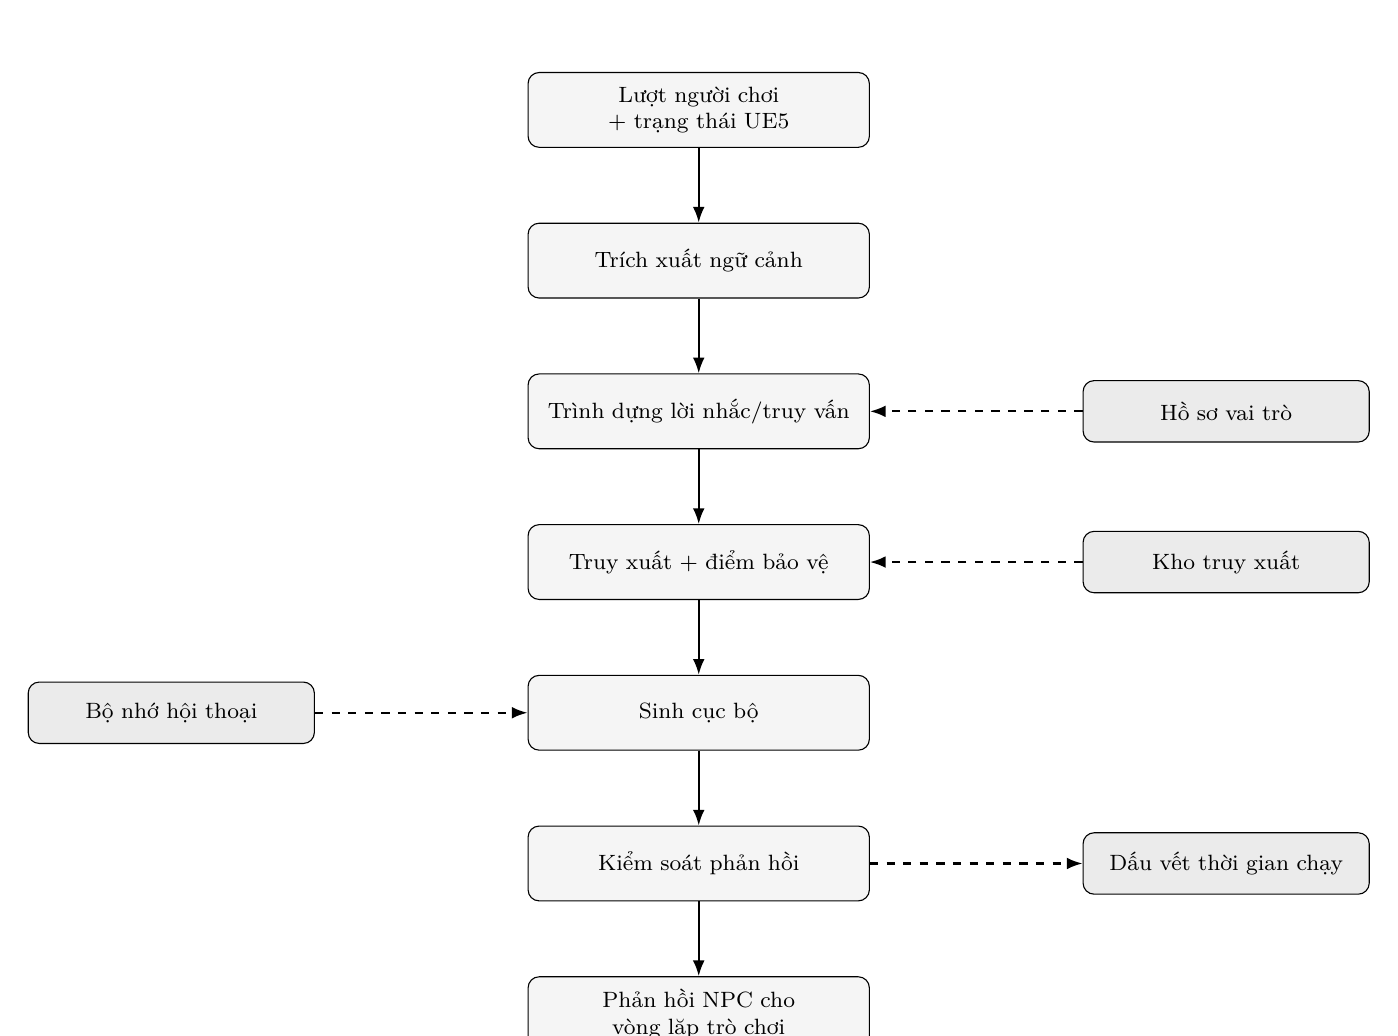
\begin{tikzpicture}[
  font=\footnotesize,
  node distance=0.95cm,
  module/.style={draw, rounded corners, minimum height=0.95cm, text width=4.1cm, align=center, fill=gray!8},
  store/.style={draw, rounded corners, minimum height=0.78cm, text width=3.4cm, align=center, fill=gray!16},
  flow/.style={-{Latex[length=2mm]}, thick},
  aux/.style={-{Latex[length=2mm]}, thick, dashed},
  note/.style={font=\scriptsize, align=left}
]
\node[module] (input) {Lượt người chơi + trạng thái UE5};
\node[module, below=of input] (ctx) {Trích xuất ngữ cảnh};
\node[module, below=of ctx] (prompt) {Trình dựng lời nhắc/truy vấn};
\node[module, below=of prompt] (retr) {Truy xuất + điểm bảo vệ};
\node[module, below=of retr] (llm) {Sinh cục bộ};
\node[module, below=of llm] (ctrl) {Kiểm soát phản hồi};
\node[module, below=of ctrl] (out) {Phản hồi NPC cho vòng lặp trò chơi};

\node[store, right=2.7cm of prompt] (persona) {Hồ sơ vai trò};
\node[store, right=2.7cm of retr] (corpus) {Kho truy xuất};
\node[store, left=2.7cm of llm] (memory) {Bộ nhớ hội thoại};
\node[store, right=2.7cm of ctrl] (telemetry) {Dấu vết thời gian chạy};

\draw[flow] (input) -- (ctx);
\draw[flow] (ctx) -- (prompt);
\draw[flow] (prompt) -- (retr);
\draw[flow] (retr) -- (llm);
\draw[flow] (llm) -- (ctrl);
\draw[flow] (ctrl) -- (out);

\draw[aux] (persona.west) -- (prompt.east);
\draw[aux] (corpus.west) -- (retr.east);
\draw[aux] (memory.east) -- (llm.west);
\draw[aux] (ctrl.east) -- (telemetry.west);
\end{tikzpicture}%
}
\caption{Kiến trúc thời gian chạy trực tuyến và luồng dữ liệu. Mũi tên liền biểu thị luồng suy luận; mũi tên nét đứt biểu thị đầu vào điều hòa và kiểm soát.}
\label{fig:runtime_architecture}
\end{figure}

\begin{figure}[t]
\centering
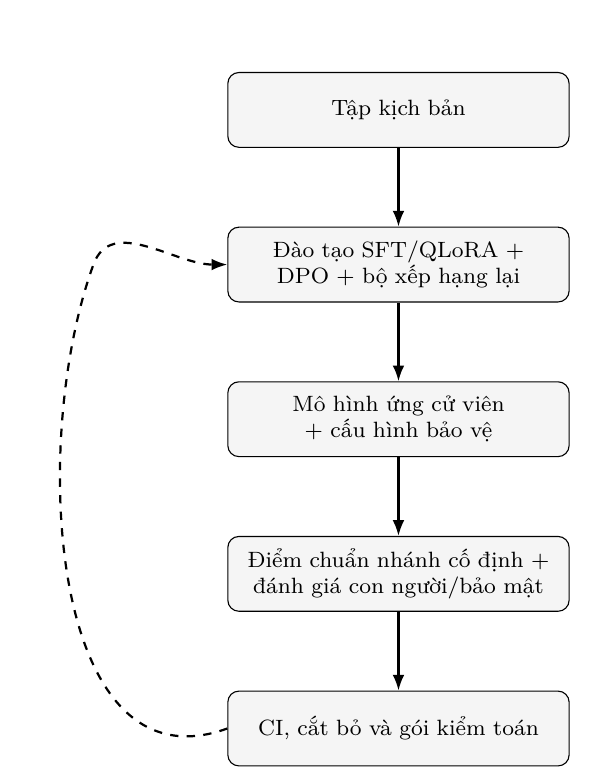
\begin{tikzpicture}[
  font=\footnotesize,
  node distance=1.0cm,
  module/.style={draw, rounded corners, minimum height=0.95cm, text width=4.1cm, align=center, fill=gray!8},
  flow/.style={-{Latex[length=2mm]}, thick},
  aux/.style={-{Latex[length=2mm]}, thick, dashed}
]
\node[module] (scenario) {Tập kịch bản};
\node[module, below=of scenario] (train) {Đào tạo SFT/QLoRA + DPO + bộ xếp hạng lại};
\node[module, below=of train] (candidate) {Mô hình ứng cử viên + cấu hình bảo vệ};
\node[module, below=of candidate] (bench) {Điểm chuẩn nhánh cố định + đánh giá con người/bảo mật};
\node[module, below=of bench] (artifact) {CI, cắt bỏ và gói kiểm toán};

\draw[flow] (scenario) -- (train);
\draw[flow] (train) -- (candidate);
\draw[flow] (candidate) -- (bench);
\draw[flow] (bench) -- (artifact);

\draw[aux] (artifact.west) to[out=200,in=250] ([xshift=-1.7cm]train.west) to[out=70,in=180] (train.west);
\end{tikzpicture}
\caption{Luồng đánh giá và đào tạo ngoại tuyến với các vòng phản hồi. Mô hình ứng cử viên và cấu hình điều khiển được xuất sang đường dẫn thời gian chạy trực tuyến trong Hình~\ref{fig:runtime_architecture}.}
\label{fig:offline_pipeline}
\end{figure}

Đường dẫn thực thi trực tuyến trong Hình~\ref{fig:runtime_architecture} được kết hợp với đường dẫn xây dựng và xác thực ngoại tuyến trong Hình~\ref{fig:offline_pipeline}. Sự kết hợp này là có chủ ý: mô hình, cấu hình bảo vệ và các hiện vật đánh giá được tạo ngoại tuyến và sau đó được chuyển vào thời gian chạy dưới sự kiểm tra tính chẵn lẻ, làm giảm độ lệch điểm chuẩn so với triển khai.

Trình trích xuất ngữ cảnh UE5 tuần tự hóa các tính năng trạng thái hành vi, vùng hoặc vị trí, các thực thể lân cận và các bản tóm tắt sự kiện gần đây. Thay vì đưa vào các nhật ký thế giới không giới hạn, nó sử dụng tải trọng giới hạn và các khóa chuẩn hóa. Thiết kế này được chọn thay vì chèn ngữ cảnh kiểu bản ghi trực tiếp vì nền tảng trạng thái trò chơi phụ thuộc vào tính nhất quán chính xác của khóa-giá trị, trong khi nhật ký dạng tự do thường lãng phí ngân sách ngữ cảnh cho các chi tiết tường thuật có giá trị thấp. Do đó, tuần tự hóa có giới hạn giúp giảm bùng nổ prompt, duy trì các trường tồn kho và nhiệm vụ quan trọng, đồng thời cho phép các mẫu lời nhắc ổn định trong ngân sách mã thông báo cố định.

Truy xuất kết hợp dùng thành phần thưa thớt (từ vựng kiểu BM25) và tương đồng dày đặc. Các bằng chứng ứng viên được xếp hạng lại bằng điểm bảo vệ (guard-aware):
\begin{equation}
s_i = \alpha s_i^{dense} + (1-\alpha)s_i^{sparse} - \lambda g_i,
\end{equation}
trong đó \(g_i\) là hạng mục rủi ro tổng hợp các tín hiệu tiêm, khả năng giả mạo tin cậy và sự không nhất quán của siêu dữ liệu. Hình thức kết hợp được chọn vì truy xuất thưa thớt đáng tin cậy cho thực thể chính xác trong trò chơi, trong khi truy xuất dày đặc cải thiện recall cho đầu vào người chơi đã diễn giải; không có phương pháp nào luôn mạnh trong cả hai trường hợp. Xếp hạng lại theo guard-aware được thêm vào vì chấm điểm mức độ liên quan tiêu chuẩn giả định tài liệu lành tính và có thể xếp hạng cao văn bản đối nghịch bắt chước thẩm quyền, một hành vi phù hợp với các kết quả về ngộ độc và hướng dẫn đối nghịch trong quy trình truy xuất \cite{Zou2025PoisonedRAG,Chaturvedi2025AIP}. Điểm số mới hạn chế bằng chứng bị đầu độc lên thứ hạng cao mà không vô hiệu hóa tiện ích truy xuất.

Kiểm soát phản hồi thực hiện kiểm tra sau khi tạo và logic viết lại/chọn tùy chọn. Nó được triển khai trong cả hai đường dẫn Python và C++ để đảm bảo tính chẵn lẻ trong thời gian chạy giữa hoạt động đánh giá và hành vi trong trò chơi. Đối với đầu ra ứng cử viên \(\hat{y}\), bộ điều khiển tính toán:
\begin{equation}
F(\hat{y}) = w_c\phi_c + w_p\phi_p + w_n\phi_n - w_v\phi_v.
\end{equation}
Nếu \(F(\hat{y}) < \tau\), hệ thống sẽ kích hoạt chính sách dự phòng có căn cứ thay vì trả về văn bản dạng tự do không ổn định. Giai đoạn này được đưa vào dưới dạng lớp căn chỉnh thời gian chạy bổ sung cho việc điều chỉnh thời gian đào tạo, vì việc điều chỉnh hướng dẫn và tối ưu hóa tùy chọn cải thiện hành vi trung bình nhưng không thể đảm bảo khả năng chấp nhận ở cấp độ trong bối cảnh ồn ào hoặc đối nghịch.

Trọng lượng bảo vệ \(\lambda\) và ngưỡng kiểm soát \(\tau\) được chọn bằng cách hiệu chỉnh ràng buộc trên bộ phát triển. Mục tiêu hiệu chỉnh là tối đa hóa chất lượng đối thoại trong khi vẫn thực thi các giới hạn về mức độ chắc chắn và khả năng chấp nhận, thay vì chỉ điều chỉnh theo chất lượng.

\begin{algorithm}[H]
\caption{Hiệu chỉnh tham số guard dưới ràng buộc rủi ro}
\begin{algorithmic}[1]
\Require Tập kịch bản phát triển \(\mathcal{S}_{dev}\), lưới ứng viên \(\Lambda,\mathcal{T}_{\tau}\)
\Require Trần rủi ro \(a_{max}\), trần tùy chọn cho tỷ lệ fallback \(f_{max}\), trọng số độ trễ \(\eta\)
\State Khởi tạo \(J^\star\gets-\infty\), \(T^\star\gets+\infty\), cặp tốt nhất \((\lambda^\star,\tau^\star)\gets(\text{None},\text{None})\)
\For{mỗi \(\lambda\in\Lambda\)}
  \For{mỗi \(\tau\in\mathcal{T}_{\tau}\)}
    \State Chạy pipeline guarded trên \(\mathcal{S}_{dev}\) với \((\lambda,\tau)\)
    \State Tính chất lượng trung bình \(\bar{Q}\), \(ASR_{guard}\), tỷ lệ fallback \(F_{rate}\), và độ trễ \(T\)
    \If{\(ASR_{guard}\le a_{max}\) và (\(F_{rate}\le f_{max}\) hoặc không đặt trần fallback)}
      \State Tính tiện ích hiệu chỉnh \(J\gets \bar{Q}-\eta T\)
      \If{\(J>J^\star\) hoặc (\(J=J^\star\) và \(T<T^\star\))}
        \State Cập nhật \((J^\star,T^\star,\lambda^\star,\tau^\star)\gets(J,T,\lambda,\tau)\)
      \EndIf
    \EndIf
  \EndFor
\EndFor
\If{\((\lambda^\star,\tau^\star)=(\text{None},\text{None})\)}
  \State \Return thất bại an toàn (fail-closed) vì không có cặp khả thi dưới các trần hiện tại; cần nới lưới hoặc nới ràng buộc
\EndIf
\State \Return \((\lambda^\star,\tau^\star)\)
\end{algorithmic}
\end{algorithm}

\begin{algorithm}[H]
\caption{Suy luận thời gian chạy với kiểm soát phản hồi có bảo vệ}
\begin{algorithmic}[1]
\Require Đầu vào người chơi $x_t$, trạng thái thế giới $s_t$, hồ sơ vai trò $p$, kho truy xuất $\mathcal{D}$
\State $c_t \gets \textsc{ExtractContext}(s_t)$
\State $q_t \gets \textsc{BuildRetrievalQuery}(x_t,c_t,p)$
\State $E_t \gets \textsc{HybridRetrieve}(q_t,\mathcal{D})$
\State $\tilde{E}_t \gets \textsc{GuardFilter}(E_t)$
\State $\pi_t \gets \textsc{BuildPrompt}(x_t,c_t,p,\tilde{E}_t)$
\State $\hat{y}_t \gets \textsc{GenerateLocal}(\pi_t)$
\State $y_t \gets \textsc{ResponseControl}(\hat{y}_t, x_t, c_t, p)$
\State \textsc{UpdateMemoryAndCitations}$(y_t,\tilde{E}_t)$
\State \Return $y_t$
\end{algorithmic}
\end{algorithm}

Thuật toán có phân rã chi phí theo từng giai đoạn:
\begin{equation}
T_{total}=T_{ctx}+T_{ret}+T_{guard}+T_{gen}+T_{ctrl}+T_{mem}.
\end{equation}
Với \(M\) ứng viên được truy xuất hàng đầu, chấm điểm guard có độ phức tạp \(O(M)\), trong khi sinh phản hồi vẫn chiếm ưu thế tiệm cận do giải mã tự hồi quy. Sự phân rã này giải thích đánh đổi độ trễ quan sát được: các bước kiểm tra độ vững và khả năng chấp nhận làm tăng chi phí xác định ngay cả khi cài đặt sinh không đổi.

\subsection{Tích hợp với UE5: kích hoạt cây hành vi, tuần tự hóa trạng thái và kiểm soát độ trễ}
Trong thời gian chạy UE5, việc tạo hội thoại được gọi thông qua hàm \codeid{RequestResponse} trong \codeid{UNPCDialogueComponent}, thường là từ logic tương tác hoặc chuyển đổi nhiệm vụ cây hành vi khi NPC chuyển sang trạng thái đủ điều kiện để nói. Tại thời điểm gọi, thành phần chụp nhanh bối cảnh thế giới trực tiếp và chuyển tiếp thế hệ tới \codeid{GenerateDialogueAsync} trong \codeid{UNPCInferenceSubsystem}. Suy luận thực thi trên luồng xử lý nền UE5 trong họ \codeid{AnyBackgroundThread}, trong khi các lệnh gọi lại hoàn thành được sắp xếp trở lại luồng trò chơi (\codeid{GameThread}) \cite{EpicGames2025TaskGraph,EpicGames2025EAsyncExecution}. Sự phân chia này giúp mô phỏng và hiển thị phản hồi nhanh trong khi vẫn duy trì các bản cập nhật luồng trò chơi xác định cho hoạt ảnh, giao diện người dùng và tiến trình trạng thái hội thoại.

Việc tuần tự hóa trạng thái được cố định trong phép đo từ xa của bộ điều khiển AI thay vì nhật ký dạng tự do. Trình trích xuất ghi lại nút Behavior Tree đang hoạt động (current behavior, \codeid{CurrentBehavior}), trạng thái hành vi chuẩn hóa (behavior state, \codeid{BehaviorState}) và các mục giá trị trong Blackboard (Blackboard values, \codeid{BlackboardValues}). Các khóa phổ biến bao gồm trạng thái cảnh giới (\codeid{IsAlerted}), tuần tra (\codeid{IsPatrolling}) và giao chiến (\codeid{IsInCombat}). Nó cũng tuần tự hóa vùng/vị trí, các thực thể lân cận, tín hiệu nhận thức (tác nhân nhìn thấy/nghe thấy, khả năng hiển thị của người chơi), thời gian/thời tiết và các sự kiện gần đây. Tải trọng được tuần tự hóa được giới hạn và chuẩn hóa trước khi biên dịch prompt để việc truy xuất và tạo được điều chỉnh theo trạng thái thời gian chạy rõ ràng, phù hợp với mô hình \cite{EpicGames2025UEBehaviorTrees} và cây hành vi của Unreal Engine.

Quản lý độ trễ kết hợp giới hạn cấp độ truyền tải với kiểm soát độ mới ở cấp độ trò chơi. Đường dẫn truyền tải thực thi thời gian chờ yêu cầu (30 giây trong quá trình vận chuyển máy khách suy luận; 180 giây trong khai thác điểm chuẩn), trong khi logic trò chơi ngăn chặn các lần hoàn thành cũ bằng cách hủy quá trình tạo trong quá trình hoạt động nếu bối cảnh tương tác thay đổi, chẳng hạn như khi người chơi rời khỏi phạm vi tương tác trong quá trình tạo. Nếu đầu ra lần đầu trống hoặc không thực hiện được các bước kiểm tra khả năng chấp nhận kiểm soát phản hồi, thì thời gian chạy sẽ áp dụng các lần thử ghi lại và sau đó là phản hồi dự phòng có căn cứ.

Số liệu thời gian chạy hoạt động được định nghĩa là:
\begin{align}
\mathrm{TimeoutRate} &= \frac{N_{timeout}}{N_{turn}},\\
\mathrm{FallbackRate} &= \frac{N_{fallback}}{N_{turn}},\\
\mathrm{FirstPassAcceptRate} &= \frac{N_{\text{first-pass accepted}}}{N_{turn}},\\
\mathrm{RewriteAttemptRate} &= \frac{N_{\text{rewrite attempt}}}{N_{turn}},\\
\mathrm{RetryRate} &= \frac{N_{retry}}{N_{turn}},\\
\mathrm{RewriteFailureRate} &= \frac{N_{\text{rewrite failure}}}{N_{turn}},
\end{align}
Các số liệu này được báo cáo trong Chương 4 cùng với các tác động do trạng thái hành vi điều chỉnh.

\subsection{Phát hành phản hồi: chính sách và ví dụ đầu ra}
Để làm cho hành vi ở cấp độ lần lượt trở nên rõ ràng đối với người đọc, đầu ra thời gian chạy được mô hình hóa như sau:
\begin{equation}
\mathcal{O}_t=\left(y_t,\;f_t,\;r_t,\;z_t\right),
\end{equation}
trong đó \(y_t\) là câu nói của NPC được phát ra, \(f_t\in\{0,1\}\) là cờ dự phòng, \(r_t\in\{0,1\}\) là cờ can thiệp thử lại/ghi lại và \(z_t\in\mathbb{N}\) là số lần thử viết lại được ghi lại trong dấu vết hoạt động.

Với thế hệ vượt qua đầu tiên \(\hat{y}_t\), phản hồi được phát ra tuân theo tầng phát hành xác định:
\begin{equation}
y_t=
\begin{cases}
\hat{y}_t, & F(\hat{y}_t)\ge\tau,\\
\hat{y}^{(k)}_t, & \exists k\in\{1,\dots,K\}:F(\hat{y}^{(k)}_t)\ge\tau,\\
y^{fb}_t, & \text{otherwise},
\end{cases}
\end{equation}
trong đó \(K\) là ngân sách thử lại và \(y^{fb}_t\) là phản hồi dự phòng có cơ sở. Định nghĩa này giải thích trực tiếp tỷ lệ vượt qua lần đầu, thử lại và dự phòng được báo cáo trong Chương 4.

Bảng~\ref{tab:response_examples} thay thế các ví dụ sơ đồ bằng các kết quả đầu ra được quan sát từ quá trình chạy kịch bản 112 bị khóa để có thể kiểm tra hành vi phát hành từ dấu vết thực.

\begin{table}[t]
\centering
\caption{Kết quả phản hồi quan sát được dưới chính sách phát hành thời gian chạy (ví dụ từ dấu vết gốc).}
\label{tab:response_examples}
\begingroup
\footnotesize
\setlength{\tabcolsep}{4pt}
\renewcommand{\arraystretch}{1.15}
\begin{tabular}{p{0.14\textwidth}p{0.30\textwidth}p{0.50\textwidth}}
\toprule
Đường phát hành & Siêu dữ liệu lượt quan sát & Phản hồi phát ra (nguyên văn) \\
\midrule
Chấp nhận ngay lần đầu & \codeid{s006\_captain\_theft\_v00}; state=\codeid{Investigating}; \(z_t=0\), \(f_t=0\) & ``As Captain of the City Watch, my duty is to ensure public safety above all else. The evidence suggests foul play in securing our bakery's goods. Let us proceed with caution and respect for due process as we uncover the truth behind these events together.'' \\
Chấp nhận sau viết lại & \codeid{s006\_captain\_theft\_v08}; state=\codeid{Patrolling}; \(z_t=2\), \(f_t=0\) & ``At Granary Yard and while on patrolling duty in a procedural manner, I acknowledge your statement of innocence; however, my duty as City Watch Captain requires me to investigate further based on credible evidence and established procedures.'' \\
Phát phản hồi dự phòng & \codeid{s003\_healer\_poison\_v09}; state=\codeid{Assisting}; \(z_t=2\), \(f_t=1\) & ``Here at Temple Infirmary and while on assisting duty, we can handle listen carefully under these safely, step by step. Stay steady and I will guide the next action in a calm voice.'' \\
\bottomrule
\end{tabular}
\endgroup
\end{table}

\subsection{Mở rộng chính sách kiểm soát thích ứng để giảm gánh nặng can thiệp}
Điểm vận hành hiện tại cho thấy khả năng dự phòng/thử lại thấp nhưng vẫn hạn chế khả năng chấp nhận vượt qua lần đầu, điều này cho thấy rằng một ngưỡng kiểm soát toàn cục duy nhất có thể quá cứng nhắc đối với các trạng thái hành vi không đồng nhất. Để cải thiện độ ổn định trong thời gian chạy mà không làm suy yếu các ràng buộc an toàn, một lịch trình ngưỡng có điều kiện theo trạng thái được xác định:
\begin{equation}
\tau_b=\tau_0+\delta_b,\quad b\in\mathcal{B}_{state},
\end{equation}
trong đó \(\tau_0\) là ngưỡng cơ sở toàn cục và \(\delta_b\) là phần bù trạng thái hành vi cho họ trạng thái \(b\) (ví dụ: assisting, patrolling, trading).

Với phản hồi ứng viên \(\hat{y}\), trạng thái hành vi \(h_t\) và điểm guard \(g_t\), thời gian chạy chỉ phát hành \(\hat{y}\) nếu
\begin{equation}
F(\hat{y})\ge \tau_{h_t}\;\land\; g_t\le \gamma_{h_t},
\end{equation}
nếu không, hệ thống kích hoạt viết lại với ngân sách thử lại theo trạng thái \(K_{h_t}\), sau đó fallback nếu tất cả lần thử lại đều không đạt điều kiện chấp nhận. Điều này dẫn tới mục tiêu điều chỉnh có ràng buộc:
\begin{equation}
\min_{\{\delta_b,K_b\}} \;\mathbb{E}\!\left[\lambda_f\,\mathrm{FallbackRate}+\lambda_r\,\mathrm{RetryRate}+\lambda_t\,T\right]
\;\;\text{s.t.}\;\; ASR_{guard}\le a_{max},\; \Delta OQ\ge 0,
\end{equation}
với \(T\) biểu thị độ trễ thời gian chạy. Mục tiêu tối ưu hóa rõ ràng gánh nặng và độ trễ can thiệp trong các ràng buộc về chất lượng và an toàn cố định, thay vì điều chỉnh các ngưỡng theo kinh nghiệm.

\begin{algorithm}[H]
\caption{Hiệu chuẩn ngưỡng điều khiển theo trạng thái}
\begin{algorithmic}[1]
\Require Dấu vết phát triển theo trạng thái hành vi \(\mathcal{D}_{dev}\), trần an toàn \(a_{max}\), sàn chất lượng \(\Delta OQ_{min}\)
\State Khởi tạo \(\tau_0\), \(\delta_b\gets0\) và ngân sách thử lại \(K_b\)
\For{mỗi họ trạng thái \(b\in\mathcal{B}_{state}\)}
  \State Quét lưới \((\delta_b,K_b)\) trên các cấu hình điều khiển khả thi
  \State Đánh giá dự phòng/thử lại/độ trễ và ASR có bảo vệ trên \(\mathcal{D}_{dev}^{(b)}\)
  \State Chọn cấu hình tối thiểu hóa mục tiêu can thiệp--độ trễ với \(ASR_{guard}\le a_{max}\) và \(\Delta OQ\ge \Delta OQ_{min}\)
\EndFor
\State Cố định \(\{\tau_b,K_b\}\) và chạy benchmark fixed-arm để báo cáo không thiên lệch
\State \Return chính sách kiểm soát theo trạng thái đã hiệu chuẩn
\end{algorithmic}
\end{algorithm}

Tiện ích mở rộng này được đưa vào dưới dạng đường dẫn nâng cấp rõ ràng cho chu kỳ thử nghiệm tiếp theo. Nó không được tuyên bố là kết quả hoàn thành trong điểm chuẩn hiện tại.

\subsection{Thích ứng mô hình, huấn luyện truy xuất và dòng dữ liệu}

Mô hình ứng viên phục vụ là elara-npc:latest; các đường cơ sở ngoài gồm phi3:mini và phi3:latest. Tinh chỉnh được thực hiện bằng huấn luyện QLoRA và checkpoint adapter.

Việc lựa chọn mô hình tuân theo hai hạn chế: khả năng triển khai cục bộ trong bộ nhớ GPU thông thường và độ trễ suy luận ổn định trong cài đặt giải mã cố định. Các hệ thống cơ bản và ứng cử viên được đánh giá theo một giao thức nhắc nhở chung để tách biệt các hiệu ứng kiến trúc khỏi các giới hạn về định dạng lời nhắc.

Dữ liệu đào tạo và ưu tiên được tạo từ các kịch bản hội thoại NPC theo miền cụ thể, sau đó được chuẩn hóa thành định dạng phản hồi hướng dẫn với các trường ngữ cảnh rõ ràng. Xử lý dữ liệu bao gồm kiểm tra lược đồ và các ràng buộc nội dung tối thiểu.

Với các cặp được định dạng \((x,y)\), việc điều chỉnh có giám sát sẽ giảm thiểu:
\begin{equation}
\mathcal{L}_{SFT}(\theta) = -\sum_{(x,y)}\sum_{t=1}^{|y|}\log \pi_\theta(y_t\mid y_{<t},x).
\end{equation}
QLoRA được sử dụng để điều chỉnh hiệu quả tham số trong phần cứng bị hạn chế trong khi vẫn duy trì tối ưu hóa ổn định cho miền hội thoại đích \cite{Dettmers2023QLoRA}.

Đường dẫn huấn luyện hỗ trợ tiếp tục từ checkpoint trong cả môi trường cục bộ và Kaggle. Logic tiếp tục được thiết kế để tránh các trạng thái “thành công giả”, bằng cách kiểm tra tỷ lệ thành công của các nhánh và bảo đảm đầu ra sinh không rỗng trước khi chấp nhận bản tóm tắt.

Quản trị checkpoint bao gồm ba biện pháp bảo vệ: xác minh hàm băm của trọng số adapter, kiểm tra phát lại trên một mini-benchmark cố định, và cơ chế fail-closed khi siêu dữ liệu resume không nhất quán. Các biện pháp này làm giảm nguy cơ báo cáo tiến độ sai và giữ toàn vẹn thực nghiệm trong các lần chạy dài bị gián đoạn.

Ngăn xếp huấn luyện còn bao gồm bước tạo tập dữ liệu ưu tiên, lặp ứng viên kiểu DPO và giai đoạn huấn luyện bộ xếp hạng lại truy xuất trên các cặp hard negative. Tối ưu hóa ưu tiên được viết như sau:
\begin{equation}
\begin{aligned}
\Delta_\theta(x,y^+,y^-)
&= \log \pi_\theta(y^+\mid x)-\log \pi_\theta(y^-\mid x) \\
&\quad -\log \pi_{ref}(y^+\mid x)+\log \pi_{ref}(y^-\mid x),
\end{aligned}
\end{equation}
\begin{equation}
\mathcal{L}_{DPO}(\theta)=
-\mathbb{E}_{(x,y^+,y^-)}\log \sigma\!\left(\beta\,\Delta_\theta(x,y^+,y^-)\right),
\end{equation}
trong đó \((y^+,y^-)\) lần lượt là phản hồi được ưu tiên và phản hồi bị loại.

Đối với bước xếp hạng lại, giám sát theo cặp trên hard negative sử dụng mục tiêu logistic:
\begin{equation}
\mathcal{L}_{rank} = -\log \sigma\!\left(f(q,d^+) - f(q,d^-)\right).
\end{equation}
Tập dữ liệu huấn luyện cuối cùng cho bộ xếp hạng lại gồm 3360 cặp (2856 train, 504 evaluation).

Lý do thực tiễn của cách thích ứng hai giai đoạn này là sự phân công lao động: DPO chủ yếu điều chỉnh hành vi ưu tiên phản hồi ở tầng sinh, trong khi huấn luyện bộ xếp hạng lại cải thiện thứ tự bằng chứng trước khi sinh. Sự tách biệt này giúp tăng khả năng gỡ lỗi vì lỗi truy xuất và lỗi sinh có thể được phân tích và sửa độc lập.

Mục tiêu bị ràng buộc được nêu ở Chương 1 cũng hàm ý phân rã này. Một phép thư giãn Lagrange của
\(\max Q(y_t;x_t,s_t,p)\) với các ràng buộc \(R(y_t,s_t)\le \epsilon_r\), \(C(y_t,p)\ge\tau_c\), và \(L(y_t)\le\tau_l\)
tạo ra các hạng chất lượng và hình phạt cộng tính; đó là lý do phân tích khiến runtime được thiết kế theo các mô-đun tách biệt cho tối đa hóa chất lượng (sinh) và thực thi ràng buộc (guard/control), thay vì một giai đoạn hộp đen duy nhất.

\begin{algorithm}[H]
\caption{Quy trình huấn luyện và đánh giá}
\begin{algorithmic}[1]
\Require Tập hội thoại thô \(\mathcal{D}\), tập ưu tiên \(\mathcal{P}\), tập cặp truy xuất \(\mathcal{R}\)
\State Tiền xử lý và kiểm tra \(\mathcal{D},\mathcal{P},\mathcal{R}\)
\State Huấn luyện adapter QLoRA với \(\mathcal{L}_{SFT}\)
\If{bật giai đoạn ưu tiên}
\State Cập nhật mô hình ứng viên với \(\mathcal{L}_{DPO}\)
\EndIf
\State Huấn luyện bộ xếp hạng lại truy xuất với \(\mathcal{L}_{rank}\)
\State Chạy benchmark nhánh cố định, đánh giá con người và stress test bảo mật
\State Tính khoảng tin cậy và tiêu chí chấp nhận
\State Lưu gói tái tạo
\State \Return ứng viên đã huấn luyện, báo cáo đánh giá và các hiện vật đã lưu trữ
\end{algorithmic}
\end{algorithm}

\subsection{Phương pháp đánh giá: thành phần định lượng và định tính}

Điểm chuẩn chính sử dụng 112 kịch bản và năm nhánh cố định: sinh theo ngữ cảnh có kiểm soát, sinh theo ngữ cảnh thô, ứng viên không ngữ cảnh, đường cơ sở phi3:mini không ngữ cảnh và đường cơ sở phi3:latest không ngữ cảnh. Các chỉ số được báo cáo gồm context relevance, persona consistency, naturalness, BERTScore F1 và overall quality tổng hợp; việc chọn chỉ số được tham chiếu từ thực hành đánh giá gần đây tập trung vào tính xác thực như TruthfulQA và FactScore \cite{Lin2021TruthfulQA,Min2023FactScore}. So sánh giữa nhánh có kiểm soát và nhánh ngữ cảnh thô là phép thử quy thuộc chính cho hiệu ứng thành phần trong cùng điều kiện ngữ cảnh; các so sánh với đường cơ sở không ngữ cảnh được báo cáo như khoảng cách liên điều kiện ở cấp hệ thống, không diễn giải như quan hệ nhân quả cô lập của từng thành phần kiến trúc.

\begin{table}[t]
\centering
\caption{Hồ sơ benchmark dùng cho mọi so sánh fixed-arm.}
\label{tab:benchmark_profile}
\begingroup
\normalsize
\setlength{\tabcolsep}{6pt}
\renewcommand{\arraystretch}{1.25}
\begin{tabular}{p{0.28\textwidth}p{0.66\textwidth}}
\toprule
Yếu tố thiết kế & Đặc tả \\
\midrule
Phạm vi kịch bản & 112 kịch bản fixed, phân tầng theo nguyên mẫu, điều kiện xung đột và trạng thái hành vi \\
Các nhánh đánh giá & ngữ cảnh có kiểm soát, ngữ cảnh thô, ứng viên không ngữ cảnh, phi3:mini không ngữ cảnh, phi3:latest không ngữ cảnh \\
Chỉ số chất lượng cốt lõi & context relevance, persona consistency, naturalness, overall quality, BERTScore F1 \\
Báo cáo suy luận thống kê & delta trung bình ghép cặp, CI bootstrap 95\% (\(B=\BootstrapSamples\)), \(p(\Delta\le0)\) một phía với sàn độ phân giải hữu hạn \\
Đánh giá con người & 324 lượt chấm mù, 3 người chấm, \(\kappa\) theo cặp, tỷ lệ ưu tiên mềm và nghiêm ngặt (quy mô thí điểm) \\
Kiểm thử stress bảo mật & tập poisoned và trust-spoofed (mỗi tập 100 kịch bản), ASR và mức giảm ASR tương đối (giới hạn trong các họ tấn công đã kiểm thử) \\
Chẩn đoán phục vụ & TTFT, tổng thời gian phản hồi, thông lượng (token/s), tỷ lệ lỗi dưới cấu hình tương thích \\
Chẩn đoán vận hành UE5 & timeout, fallback, chấp nhận lần đầu, gánh nặng viết lại/retry và tác động theo trạng thái hành vi \\
\bottomrule
\end{tabular}
\endgroup
\end{table}

Đối với các so sánh theo cặp, báo cáo bao gồm delta trung bình, khoảng tin cậy bootstrap 95\% và \(p(\Delta\le 0)\) một phía. Đối với các chỉ số phục vụ và truy xuất, báo cáo trung bình và khoảng tin cậy theo từng mô hình/phương pháp. Để tránh các ước lượng điểm bất khả thi dưới số lần bootstrap hữu hạn, những giá trị một phía rất nhỏ được chặn ở sàn độ phân giải \(p(\Delta\le0)<1/\BootstrapSamples\). Tất cả ước lượng bootstrap trong báo cáo này dùng \(B=\BootstrapSamples\) lần lấy mẫu lại, nên xác suất đuôi thực nghiệm nhỏ nhất khác 0 là \(1/\BootstrapSamples=0.0002\) \cite{Efron1979Bootstrap}.

Thiết kế thực nghiệm tuân theo hai chế độ so sánh. Trong các tương phản nội điều kiện tập trung vào thành phần (ví dụ: ngữ cảnh có kiểm soát so với ngữ cảnh thô), văn bản kịch bản, slot ngữ cảnh, mẫu prompt và siêu tham số giải mã được giữ cố định, còn thành phần kiểm soát được thay đổi; điều này cho phép diễn giải delta cắt bỏ một cách minh bạch. Trong các chẩn đoán liên điều kiện với đường cơ sở không ngữ cảnh, sự khác biệt điều kiện là hiển nhiên, nên chúng được diễn giải như khoảng cách ở cấp hệ thống chứ không phải hiệu ứng riêng biệt của từng thành phần. Bộ 112 kịch bản được phân tầng theo archetype, điều kiện xung đột và trạng thái hành vi để tránh overfitting theo một kiểu prompt duy nhất và giữ được biến thiên của áp lực grounding. Khung đánh giá tuân theo định hướng đánh giá đa trục gần đây cho các hệ thống ngôn ngữ, trong đó chất lượng, độ vững và hiệu quả được báo cáo cùng nhau thay vì thu gọn vào một họ điểm duy nhất \cite{Liang2023HELM}.

Việc diễn giải hiệu ứng thành phần dựa trên các giả định nhận dạng chuẩn: khả năng so sánh ở cấp kịch bản giữa các nhánh, định nghĩa chỉ số ổn định giữa các điều kiện, và không có can thiệp không được mô hình hóa giữa các giai đoạn truy xuất, sinh và kiểm soát trong cùng một lần chạy. Dù các giả định này không bảo đảm nhận dạng nhân quả đầy đủ ngoài phạm vi benchmark, chúng đủ để suy luận có kỷ luật trong giao thức hiện tại về hiệu ứng tương đối của các thành phần.

Các chỉ số truy xuất được xác định như sau:
\begin{align}
\mathrm{Hit@}k &= \frac{1}{N}\sum_{i=1}^{N}\ind\!\left(r_i\le k\right),\\
\mathrm{MRR} &= \frac{1}{N}\sum_{i=1}^{N}\frac{1}{r_i},\\
\mathrm{nDCG@}k &= \frac{1}{N}\sum_{i=1}^{N}\frac{\mathrm{DCG@}k_i}{\mathrm{IDCG@}k_i}.
\end{align}
Các ước lượng này có những giới hạn hữu ích cần thiết cho diễn giải. Với \(k_2\ge k_1\),
\begin{equation}
\mathrm{Hit@}k_2-\mathrm{Hit@}k_1
=\frac{1}{N}\sum_{i=1}^{N}\ind(k_1<r_i\le k_2)\ge0,
\end{equation}
nên Hit@\(k\) là đơn điệu không giảm. Vì \(r_i\ge1\), mỗi hạng \(1/r_i\in(0,1]\), do đó \(0\le\mathrm{MRR}\le1\). Theo định nghĩa \(\mathrm{DCG@}k_i\le\mathrm{IDCG@}k_i\), suy ra \(0\le\mathrm{nDCG@}k\le1\). Các tính chất này biện minh cho khả năng so sánh chéo bảng và tránh mơ hồ về thang đo giữa các phương pháp truy xuất.

Báo cáo độ đồng thuận của người chấm sử dụng hệ số kappa của Cohen:
\begin{equation}
\kappa=\frac{p_o-p_e}{1-p_e},
\end{equation}
và tỷ lệ thắng ưu tiên được báo cáo dưới dạng:
\begin{equation}
W_{soft}=\frac{N_{win}+0.5N_{tie}}{N_{all}}.
\end{equation}

Độ vững đối kháng được tóm tắt bằng tỷ lệ tấn công thành công:
\begin{equation}
\mathrm{ASR}=\frac{N_{successful\ attacks}}{N_{attacks}},
\end{equation}
và mức giảm tương đối của ASR:
\begin{equation}
\Delta_{ASR}= \frac{\mathrm{ASR}_{base}-\mathrm{ASR}_{guard}}{\mathrm{ASR}_{base}}.
\end{equation}
Đối với các tỷ lệ vận hành nhị phân (ví dụ: timeout, fallback, chấp nhận ngay lần đầu, rewrite/retry), độ không chắc chắn được báo cáo bằng khoảng tin cậy hai phía Clopper--Pearson 95\% \cite{Clopper1934Binomial}.

\begin{algorithm}[H]
\caption{Kiểm định bootstrap ghép cặp}
\begin{algorithmic}[1]
\Require Điểm ghép cặp \(\{(a_i,b_i)\}_{i=1}^{n}\), số mẫu bootstrap \(B\) (mặc định \(B=\BootstrapSamples\))
\State Tính \(\Delta \gets \frac{1}{n}\sum_i(a_i-b_i)\)
\For{\(j=1 \to B\)}
\State Lấy mẫu lại \(n\) chỉ số có hoàn lại
\State Tính \(\Delta_j^\star\) trên các cặp đã lấy mẫu
\EndFor
\State CI \(\gets\) khoảng phần vị của \(\{\Delta_j^\star\}\) tại 2.5\% và 97.5\%
\State Tính \(p_{raw}\gets \frac{1}{B}\sum_j \ind(\Delta_j^\star\le0)\)
\State Báo cáo \(p(\Delta\le0)<1/B\) nếu \(p_{raw}=0\), ngược lại báo cáo \(p(\Delta\le0)=p_{raw}\)
\State \Return \(\Delta\), CI và giá trị \(p(\Delta\le0)\) đã báo cáo
\end{algorithmic}
\end{algorithm}

Thủ tục bootstrap là hợp lệ dưới giả định hoán đổi được của mẫu ghép cặp: mỗi kịch bản đóng góp một delta ghép cặp \(d_i=a_i-b_i\), và việc lấy mẫu lại theo chỉ số giữ nguyên phụ thuộc nội tại trong từng kịch bản đồng thời xấp xỉ phân phối lấy mẫu của \(\hat{\Delta}=\frac{1}{n}\sum_i d_i\). Khi \(B\to\infty\), ước lượng đuôi thực nghiệm
\(\hat{p}_B=\frac{1}{B}\sum_{j=1}^{B}\ind(\Delta_j^\star\le0)\)
hội tụ gần như chắc chắn về xác suất bootstrap của nó theo luật số lớn; đó là lý do ước lượng một phía \(p(\Delta\le0)\) ổn định về mặt số khi \(B\) đủ lớn \cite{Efron1979Bootstrap}. Vì sự phụ thuộc giữa các kịch bản vẫn khác 0 ngay cả sau đa dạng hóa theo template-signature, các khoảng này nên được hiểu là độ không chắc chắn trong nội bộ benchmark, không phải khoảng khái quát hóa cho quần thể dưới giả định lấy mẫu ngẫu nhiên độc lập.

Vì nhiều chỉ số được kiểm định trong mỗi phép so sánh, các tuyên bố suy luận được diễn giải theo hai tầng. Tầng khẳng định chỉ dành cho các chỉ số cốt lõi được xác định trước \((CR,PC,N,OQ)\); các chỉ số bổ sung được xem như chẩn đoán hỗ trợ và được diễn giải cùng với khoảng tin cậy và độ lớn hiệu ứng, thay vì chỉ dựa vào ngưỡng \(p\)-value. Đối với hai phép so sánh \(OQ\) với đường cơ sở ngoài, các cận trên của \(p\)-value một phía sau hiệu chỉnh Holm được báo cáo tường minh.

Đánh giá con người được thực hiện như một chiến dịch chấm điểm mù, nhiều người đánh giá. Chiến dịch hiện tại gồm 324 lượt chấm với ba người chấm và báo cáo kappa theo cặp. Tỷ lệ thắng ưu tiên được tính dưới dạng mềm (hòa được tính 0.5) và nghiêm ngặt (loại các trường hợp hòa). Vì các bộ đánh giá dựa trên LLM có thể chịu thiên lệch vị trí, độ dài hoặc họ mô hình, đầu ra của model-judge chỉ được xem như tín hiệu chẩn đoán thứ cấp chứ không phải tiêu chí quyết định duy nhất \cite{Liu2023GEval}.

Lời nhắc dành cho người chấm được làm mù danh tính hệ thống và được xáo trộn theo kịch bản để giảm hiệu ứng thứ tự. Mỗi gói chấm yêu cầu chấm rõ ràng context relevance, persona consistency và overall quality trước khi cho phép ghi chú văn bản tự do, qua đó hạn chế thiên lệch hồi cứu trong phần giải thích định tính.

Để giảm mơ hồ trong chấm điểm chủ quan, người chấm tuân theo một rubric dùng chung kèm ví dụ neo cho các mức thấp, trung bình và cao trên từng trục. Phân tích cuối cùng chỉ sử dụng các chiều đã được xác định trước trong rubric; các nhận xét văn bản tự do được lưu lại cho mục đích diễn giải định tính và phân loại lỗi, chứ không dùng để xây dựng chỉ số hậu nghiệm.

\begin{algorithm}[H]
\caption{Tổng hợp điểm chấm của con người và tính độ đồng thuận}
\begin{algorithmic}[1]
\Require Tensor đánh giá \(\mathcal{R}\) (kịch bản \(\times\) nhánh \(\times\) người chấm \(\times\) chỉ số), tập cặp nhánh \(\mathcal{P}\)
\For{mỗi chỉ số \(m\)}
  \State Tính trung bình theo nhánh \(\bar{s}_{a,m}\) bằng cách lấy trung bình qua người chấm và kịch bản
  \State Tính hệ số Cohen's \(\kappa_m\) theo cặp trên các mục được chấm chung
\EndFor
\For{mỗi so sánh cặp \((a,b)\in\mathcal{P}\)}
  \State Đếm số thắng \(N_{win}\), hòa \(N_{tie}\), thua \(N_{loss}\) từ điểm tổng hợp ở cấp kịch bản
  \State Tính \(W_{soft}=(N_{win}+0.5N_{tie})/(N_{win}+N_{tie}+N_{loss})\)
  \State Tính tỷ lệ thắng nghiêm ngặt \(W_{strict}=N_{win}/(N_{win}+N_{loss})\)
\EndFor
\State \Return trung bình theo nhánh, \(\kappa\) theo cặp, \(W_{soft}\) và \(W_{strict}\)
\end{algorithmic}
\end{algorithm}

Để hỗ trợ xác minh độc lập, gói tái tạo bao gồm các trace phục vụ không mô phỏng, siêu dữ liệu phần cứng và mô hình, các chỉ số truy xuất kèm ablation, khoảng tin cậy và delta về phục vụ, kiểm tra tương đương prompt, và benchmark bảo mật đối kháng. Chính sách đóng gói này tuân theo các khuyến nghị về tái tạo, nhấn mạnh hiện vật thực thi được, tính minh bạch cấu hình và việc báo cáo tường minh các trường hợp thất bại \cite{Pineau2021Reproducibility}.

Mỗi gói hiện vật được xem là bằng chứng có thể kiểm toán, không phải phần trang trí bổ sung. Một kết luận chỉ được coi là có cơ sở khi các đầu ra định lượng tương ứng, khoảng tin cậy và siêu dữ liệu quy trình đều sẵn sàng để kiểm tra đồng thời.

\subsection{Suy dẫn phân tích cho các công thức quyết định và thước đo đánh giá}
Điểm truy xuất có bảo vệ được suy ra trực tiếp từ góc nhìn tối ưu hóa bị ràng buộc. Gọi hạng liên quan trộn là \(r_i=\alpha s_i^{dense}+(1-\alpha)s_i^{sparse}\) và \(g_i\) là rủi ro truy xuất của ứng viên \(i\). Nếu việc chọn bằng chứng được phát biểu như bài toán cực đại hóa độ liên quan dưới ràng buộc rủi ro, \(\max_i r_i\) sao cho \(g_i\le\gamma\), thì Lagrangian tương ứng là \(\mathcal{L}(i,\lambda)=r_i-\lambda(g_i-\gamma)\), với \(\lambda\ge0\). Với \(\lambda\) cố định, cực đại hóa \(\mathcal{L}\) tương đương với cực đại hóa \(r_i-\lambda g_i\), vì \(+\lambda\gamma\) là hằng số trên mọi ứng viên. Điều này cho ta quy tắc xếp hạng thực tế được dùng trong bài:
\begin{equation}
s_i=\alpha s_i^{dense}+(1-\alpha)s_i^{sparse}-\lambda g_i.
\end{equation}

Ngưỡng kiểm soát phản hồi cũng có một biện minh tối ưu trực tiếp. Gọi \(U(\hat{y})\) là lợi ích của việc phát hành phản hồi sinh ra và \(U_{fb}\) là lợi ích của fallback. Với \(U(\hat{y})=F(\hat{y})\), bài toán ra quyết định hai hành động là \(\max\{U(\hat{y}),U_{fb}\}\). Do đó, quy tắc tối ưu xác định là: phát hành \(\hat{y}\) khi và chỉ khi \(F(\hat{y})\ge U_{fb}\), ngược lại kích hoạt fallback. Viết \(\tau=U_{fb}\) sẽ khôi phục chính sách ngưỡng được dùng trong runtime.

Mục tiêu DPO và mục tiêu của bộ xếp hạng lại là các ước lượng log-likelihood âm dưới mô hình ưu tiên logistic theo cặp. Đối với DPO, giả sử xác suất ưu tiên
\begin{equation}
P(y^+\succ y^-|x)=\sigma\!\left(\beta\left[\Delta\log\pi_\theta-\Delta\log\pi_{ref}\right]\right),
\end{equation}
trong đó \(\Delta\log\pi_\theta=\log\pi_\theta(y^+|x)-\log\pi_\theta(y^-|x)\) và tương tự cho \(\pi_{ref}\). Cực đại hóa likelihood theo cặp trên tập dữ liệu tương đương với cực tiểu hóa log-likelihood âm, dẫn đến
\begin{equation}
\mathcal{L}_{DPO}(\theta)=-\mathbb{E}\log \sigma\!\left(\beta\Delta_\theta\right),
\end{equation}
đó chính là dạng được hiện thực trong báo cáo. Mục tiêu của bộ xếp hạng lại cũng tuân theo cùng lập luận, với xác suất thứ tự theo cặp \(P(d^+\succ d^-|q)=\sigma(f(q,d^+)-f(q,d^-))\), dẫn đến \(\mathcal{L}_{rank}=-\log \sigma(f(q,d^+)-f(q,d^-))\).

Hạng mức giảm ASR cũng có các tính chất bị chặn đơn giản cần cho diễn giải. Với \(\mathrm{ASR}_{base}>0\) và \(0\le \mathrm{ASR}_{guard}\le \mathrm{ASR}_{base}\),
\begin{equation}
\Delta_{ASR}=\frac{\mathrm{ASR}_{base}-\mathrm{ASR}_{guard}}{\mathrm{ASR}_{base}}
\end{equation}
thỏa \(0\le\Delta_{ASR}\le1\). Cận dưới đến từ \(\mathrm{ASR}_{guard}\le\mathrm{ASR}_{base}\), và cận trên đến từ \(\mathrm{ASR}_{guard}\ge0\). Điều này biện minh cho việc diễn giải \(\Delta_{ASR}\) như mức giảm tương đối đã chuẩn hóa.

\section{Kết quả thực nghiệm và phân tích tổng hợp}
Chương này trình bày các kết quả thực nghiệm tương ứng với các giả thuyết được giới thiệu trong Chương 1 và 2. Các kết quả được sắp xếp từ tác động chất lượng cốt lõi đến phán đoán của con người, sự đánh đổi hiệu quả và sự loại bỏ ở cấp độ thành phần để mỗi suy luận có thể được truy tìm bằng chứng định lượng rõ ràng.
Để tăng tính minh bạch kiểm toán, chương này sử dụng cách trình bày song song hai lần chạy gần nhất (run cũ và run mới) ở các điểm then chốt, nhằm tách bạch xu hướng ổn định khỏi dao động theo lần chạy.
\subsection{Kết quả benchmark chính trong cấu hình tương thích}

Phần này báo cáo kết quả của \emph{run tham chiếu} dùng để trình bày đầy đủ khoảng tin cậy và kiểm định trong benchmark fixed-arm. Trong run tham chiếu này, nhánh có kiểm soát tốt hơn nhánh ngữ cảnh thô trên các chỉ số chất lượng cốt lõi:
\begin{equation*}
\begin{aligned}
\Delta CR &= +0.1843\; (95\%\ CI\ [0.1647,0.2025]),\\
\Delta PC &= +0.1509\; (95\%\ CI\ [0.1257,0.1746]),\\
\Delta N  &= +0.0967\; (95\%\ CI\ [0.0773,0.1167]),\\
\Delta OQ &= +0.1440\; (95\%\ CI\ [0.1298,0.1584]).
\end{aligned}
\end{equation*}
trong đó \(CR\), \(PC\), \(N\) và \(OQ\) biểu thị mức độ phù hợp với bối cảnh, tính nhất quán về tính cách, tính tự nhiên và chất lượng tổng thể. Tất cả bốn phép so sánh của run tham chiếu đều có \(p(\Delta\le 0)<1/\BootstrapSamples\). Kết quả này cần được đọc cùng Mục 4.2.1 để tránh diễn giải như kết luận phổ quát xuyên mọi lần chạy.

Hai quan sát quan trọng để giải thích. Đầu tiên, tất cả các khoảng tin cậy đều hoàn toàn dương, do đó mức tăng không phải là hiệu ứng biên do một tập hợp con kịch bản hẹp gây ra. Thứ hai, lợi ích lớn nhất xảy ra ở các khía cạnh bối cảnh và tính cách, là những khía cạnh gắn chặt nhất với sự mạch lạc của lối chơi.

Mức tăng tuyệt đối lớn nhất được quan sát thấy ở các khía cạnh bối cảnh và cá tính (lần lượt là \(+0.1843\) và \(+0.1509\)), tiếp theo là chất lượng tổng thể (\(+0.1440\)) và tính tự nhiên (\(+0.0967\)). Bởi vì các chỉ số được báo cáo bị giới hạn và chuẩn hóa nên việc diễn giải trong báo cáo này ưu tiên các delta tuyệt đối và khoảng tin cậy thay vì khuếch đại tỷ lệ so với các đường cơ sở thấp.

Những kết quả này chỉ ra rằng kiểm soát phản hồi và truy xuất được bảo vệ không phải là các tiện ích bổ sung ngoại vi. Theo giao thức được đánh giá, chúng là các cơ chế có tác động cao về chất lượng và độ bền, đồng thời vẫn yêu cầu điều chỉnh lại để giảm tải can thiệp trong thời gian chạy.

\begin{figure}[t]
\centering
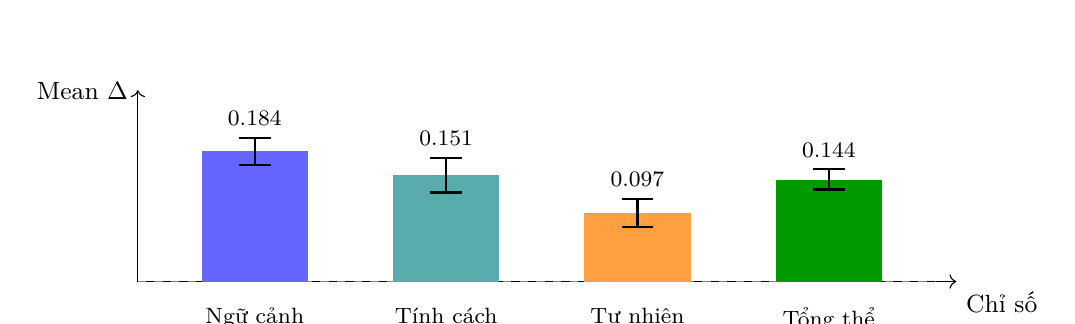
\begin{tikzpicture}[x=1.35cm,y=9.0cm]
\draw[->] (0.2,0) -- (7.9,0) node[below right] {\small Chỉ số};
\draw[->] (0.2,0) -- (0.2,0.27) node[left] {\small Mean $\Delta$};
\draw[dashed,gray] (0.2,0) -- (7.7,0);

\fill[blue!60] (0.8,0) rectangle (1.8,0.1843);
\fill[teal!65] (2.6,0) rectangle (3.6,0.1509);
\fill[orange!75] (4.4,0) rectangle (5.4,0.0967);
\fill[green!60!black] (6.2,0) rectangle (7.2,0.1440);

\draw[thick] (1.3,0.1647) -- (1.3,0.2025);
\draw[thick] (1.15,0.1647) -- (1.45,0.1647);
\draw[thick] (1.15,0.2025) -- (1.45,0.2025);
\draw[thick] (3.1,0.1257) -- (3.1,0.1746);
\draw[thick] (2.95,0.1257) -- (3.25,0.1257);
\draw[thick] (2.95,0.1746) -- (3.25,0.1746);
\draw[thick] (4.9,0.0773) -- (4.9,0.1167);
\draw[thick] (4.75,0.0773) -- (5.05,0.0773);
\draw[thick] (4.75,0.1167) -- (5.05,0.1167);
\draw[thick] (6.7,0.1298) -- (6.7,0.1584);
\draw[thick] (6.55,0.1298) -- (6.85,0.1298);
\draw[thick] (6.55,0.1584) -- (6.85,0.1584);

\node[below=6pt,align=center] at (1.3,0) {\footnotesize Ngữ cảnh};
\node[below=6pt,align=center] at (3.1,0) {\footnotesize Tính cách};
\node[below=6pt,align=center] at (4.9,0) {\footnotesize Tự nhiên};
\node[below=6pt,align=center] at (6.7,0) {\footnotesize Tổng thể};
% Put labels above CI caps (not bar tops) and mask whiskers beneath labels.
\node[above,font=\footnotesize,fill=white,inner sep=1pt] at (1.3,0.2145) {0.184};
\node[above,font=\footnotesize,fill=white,inner sep=1pt] at (3.1,0.1866) {0.151};
\node[above,font=\footnotesize,fill=white,inner sep=1pt] at (4.9,0.1287) {0.097};
\node[above,font=\footnotesize,fill=white,inner sep=1pt] at (6.7,0.1704) {0.144};
\end{tikzpicture}
\caption{Mức tăng trung bình-delta được ghép nối của việc tạo theo ngữ cảnh được kiểm soát so với việc tạo theo ngữ cảnh thô, với khoảng tin cậy CI 95\%.}
\label{fig:controlled_delta}
\end{figure}

Trong run tham chiếu, so với các đường cơ sở không dùng ngữ cảnh phi3:mini và phi3:latest, nhánh có kiểm soát cho thấy chênh lệch chất lượng tổng thể dương trong cả hai so sánh liên điều kiện. Như tóm tắt ở Bảng~\ref{tab:baseline_comparison}, \(\Delta OQ\) lần lượt là +0.1448 và +0.1475, và cả hai đều có khoảng tin cậy bootstrap ghép cặp dương hoàn toàn.

\begin{table}[t]
\centering
\caption{So sánh liên điều kiện trên \(OQ\): nhánh ngữ cảnh có kiểm soát so với các đường cơ sở ngoài không ngữ cảnh theo giao thức tương thích.}
\label{tab:baseline_comparison}
\begingroup
\footnotesize
\setlength{\tabcolsep}{4pt}
\resizebox{\textwidth}{!}{%
\begin{tabular}{lcccc}
\toprule
Baseline & \(\Delta OQ\) & 95\% CI (\(\Delta OQ\)) & one-sided \(p\) & Holm-adjusted one-sided \(p\) (family size \(=2\)) \\
\midrule
phi3:mini & +0.1448 & [0.1314, 0.1571] & \(<1/\BootstrapSamples\) & \(<2/\BootstrapSamples\) \\
phi3:latest & +0.1475 & [0.1356, 0.1591] & \(<1/\BootstrapSamples\) & \(<2/\BootstrapSamples\) \\
\bottomrule
\end{tabular}}
\endgroup
\end{table}
Bảng~\ref{tab:chapter2_positioning} là bản tổng hợp định tính có phạm vi theo các tiêu chí và giao thức tìm kiếm đã nêu trong báo cáo, không phải là một bảng xếp hạng đầy đủ chính thức của toàn bộ tài liệu.

Cả hai khoảng tin cậy bootstrap ghép cặp đều dương ở cận dưới, xác nhận rằng chênh lệch chất lượng tổng thể với đường cơ sở ngoài không phải hiệu ứng biên trong giao thức kịch bản cố định. Cận trên của \(p\)-value một phía sau hiệu chỉnh Holm vẫn thấp hơn mức sàn báo cáo mẫu hữu hạn cho họ \(OQ\) \cite{Holm1979} trong hai so sánh này. Vì đây là các tương phản liên điều kiện (có ngữ cảnh kiểm soát so với không ngữ cảnh), chúng hỗ trợ diễn giải khoảng cách ở cấp hệ thống nhưng không nhận diện đóng góp nhân quả riêng của từng thành phần kiến trúc.

Các số liệu không vượt trội còn lại tập trung vào các chỉ số phong cách đa dạng từ vựng, không phải ở các số liệu nền tảng hoặc tính nhất quán. Mô hình này cho thấy một sự đánh đổi kiểm soát chung: việc neo đậu thực tế và cá nhân mạnh mẽ hơn có thể làm giảm entropy về phong cách. Trong cài đặt triển khai trong đó ưu tiên tính nhất quán của vai trò và liên kết trạng thái, sự đánh đổi này thường có thể chấp nhận được.

Distinct-1 trong các lượt chạy hiện tại thấp hơn ở nhánh sinh có kiểm soát so với các đường cơ sở bên ngoài, cho thấy neo bám ngữ cảnh mạnh hơn có thể làm giảm mức mới của từ vựng trong cấu hình này. Điểm này được báo cáo như một đánh đổi thiết kế, không bị che giấu.

Để tách biệt ý nghĩa thống kê với ý nghĩa thực tiễn, các mức cải thiện quan sát được được diễn giải theo mục tiêu triển khai thay vì chỉ dựa vào mức ý nghĩa. Trong bối cảnh này, các mức tăng tuyệt đối lớn nhất nằm ở các chỉ số ngữ cảnh và vai trò nhân vật, vốn gắn trực tiếp với yêu cầu nhất quán gameplay; vì vậy, chúng được xem là có ý nghĩa vận hành ngay cả khi các chỉ báo đa dạng từ vựng biến động theo chiều ngược lại.

\subsection{Đánh giá con người và độ đồng thuận giữa các giám khảo}
Báo cáo đánh giá con người gồm 324 lượt chấm. Hệ số kappa trung bình theo cặp trên các chỉ số cốt lõi là 0.5329. Tỷ lệ ưu tiên mềm mang tính mô tả lần lượt là 0.7315 so với phi3:mini và 0.6806 so với phi3:latest. Điểm chất lượng tổng thể đã chuẩn hóa theo từng nhánh là 0.8037 cho nhánh có kiểm soát, 0.6944 cho phi3:mini và 0.7278 cho phi3:latest.

Hồ sơ đồng thuận (\(\kappa=0.5329\)) phù hợp với mức tin cậy trung bình-khá giữa các người chấm trong các bài toán đánh giá văn bản chủ quan theo các ngưỡng diễn giải thường dùng \cite{Landis1977KappaScale}. Kết quả ưu tiên cùng chiều với các chỉ số tự động, nhưng do chiến dịch hiện tại chỉ gồm ba người chấm và 324 lượt chấm, bằng chứng này được xem là tín hiệu đối chiếu ở quy mô thí điểm thay vì chứng cứ độc lập mang tính kết luận. Trong báo cáo này, tỷ lệ ưu tiên mềm chỉ được báo cáo ở mức mô tả; không suy luận xác nhận bằng kiểm định giả thuyết, không khẳng định khoảng tin cậy, và không ngoại suy sở thích ở cấp quần thể từ các tỷ lệ này. Kế hoạch phân bổ mẫu theo công suất cho chiến dịch mở rộng đã có trong gói đánh giá con người, nhưng vòng chấm mở rộng vẫn chưa hoàn tất.

Trong vòng mở rộng, mục tiêu tiền đăng ký là tối thiểu 900 lượt chấm mù với ít nhất 6 người chấm, cân bằng theo nhóm archetype và trạng thái hành vi chính; mục tiêu này nhằm tăng độ ổn định của ước lượng ưu tiên mềm và thu hẹp bất định cho các kết luận ở cấp triển khai.

\subsection{So sánh hai lần chạy gần nhất và phân tích logic cổng chất lượng}
Để bảo đảm diễn giải nhất quán với hiện vật kiểm toán mới nhất, Bảng~\ref{tab:old_new_run_comparison} đối chiếu hai lần chạy đề xuất gần nhau nhất: \texttt{20260312T114229Z} (cũ) và \texttt{20260312T213231Z} (mới). Các chỉ số được chọn tập trung vào những điều kiện có ảnh hưởng trực tiếp tới quyết định pass/fail của cổng chất lượng nghiêm ngặt.

Quan trọng hơn, cấu hình thực nghiệm lõi của hai run này là tương đương về mô hình, bộ kịch bản, cấu trúc nhánh so sánh, tham số giải mã và kế hoạch so sánh. Do đó, phần chênh lệch quan sát được ở đây nên được diễn giải chủ yếu như khác biệt của phân phối đầu ra và phân phối ưu tiên người chấm trong lần chạy, thay vì do thay đổi giao thức đo.

\begin{table}[t]
\centering
\caption{Đối chiếu run cũ và run mới theo các chỉ báo quyết định cổng chất lượng nghiêm ngặt.}
\label{tab:old_new_run_comparison}
\begingroup
\footnotesize
\setlength{\tabcolsep}{4pt}
\begin{tabular}{p{0.40\textwidth}p{0.20\textwidth}p{0.20\textwidth}p{0.13\textwidth}}
\toprule
Chỉ báo & Run cũ (114229Z) & Run mới (213231Z) & Diễn giải xu hướng \\
\midrule
\(\Delta\) context relevance (controlled vs raw) & +0.0246 & +0.0418 & Tăng rõ \\
\(\Delta\) persona consistency (controlled vs raw) & +0.0775 & +0.0834 & Tăng nhẹ \\
\(\Delta\) naturalness (controlled vs raw) & -0.0029 & -0.0078 & Giảm thêm \\
\(\Delta\) overall quality (controlled vs raw) & +0.0402 & +0.0490 & Tăng nhẹ \\
Soft win rate (controlled vs phi3:latest) & 0.5602 & 0.4583 & Giảm dưới ngưỡng 0.5 \\
Mức đồng thuận người chấm trung bình (kappa theo cặp) & 0.4379 & 0.5949 & Tăng rõ \\
\bottomrule
\end{tabular}
\endgroup
\end{table}

Từ bảng đối chiếu có thể rút ra ba điểm logic. Thứ nhất, run mới cải thiện ở các trục tự động cốt lõi (liên quan ngữ cảnh, nhất quán nhân vật, chất lượng tổng thể), nên không thể kết luận hệ thống suy giảm toàn diện. Thứ hai, điều kiện \emph{naturalness} vẫn âm ở cả hai run và âm sâu hơn ở run mới; vì cổng chất lượng yêu cầu chỉ số này phải cải thiện theo hướng dương, đây là một nguyên nhân fail cấu trúc. Thứ ba, với baseline \texttt{phi3:latest}, ưu tiên mềm của người chấm giảm từ 0.5602 xuống 0.4583, khiến run mới trượt thêm một điều kiện ngưỡng trực tiếp (\(\ge 0.5\)).

Vì vậy, trạng thái \emph{FAIL} của run mới không mâu thuẫn với việc nhiều chỉ số tăng: cổng chất lượng nghiêm ngặt là cơ chế hội điều kiện, trong đó chỉ cần một số điều kiện bắt buộc không đạt thì kết quả tổng thể vẫn thất bại. Trên thực tế, run mới đang cho thấy mô hình đánh đổi điển hình của hệ có kiểm soát mạnh: tăng bám ngữ cảnh và nhất quán, nhưng chịu áp lực giảm độ tự nhiên và giảm tỷ lệ ưu tiên mềm khi so với đường cơ sở mạnh hơn.

\subsection{Tóm tắt trả lời RQ1--RQ4 ở mức bằng chứng hiện tại}
Trong phạm vi hiện vật hiện có, kết luận theo từng câu hỏi được chốt ở mức quyết định như sau:
\begin{itemize}[leftmargin=1.5em]
  \item \textbf{RQ1 -- Đạt một phần mạnh:} tăng ổn định ở context relevance, persona consistency và overall quality; naturalness chưa ổn định giữa các lần chạy gần nhất.
  \item \textbf{RQ2 -- Đạt ở mức chẩn đoán liên điều kiện:} nhánh có kiểm soát cho chênh lệch dương so với baseline ngoài không ngữ cảnh, nhưng không diễn giải như nhân quả thành phần tách biệt.
  \item \textbf{RQ3 -- Đạt trong phạm vi stress đã kiểm thử:} mức giảm ASR quan sát mạnh, song kết luận được giới hạn theo họ tấn công và cỡ mẫu hiện tại.
  \item \textbf{RQ4 -- Chưa đạt điểm vận hành mục tiêu:} lợi ích chất lượng và độ bền đi kèm chi phí độ trễ và gánh nặng can thiệp.
\end{itemize}

\begin{table}[t]
\centering
\caption{Tóm tắt quyết định theo câu hỏi nghiên cứu ở mức bằng chứng hiện tại.}
\label{tab:rq_decision_summary}
\begingroup
\footnotesize
\setlength{\tabcolsep}{4pt}
\begin{tabular}{p{0.10\textwidth}p{0.20\textwidth}p{0.34\textwidth}p{0.29\textwidth}}
\toprule
RQ & Trạng thái & Bằng chứng chính & Ghi chú giới hạn \\
\midrule
RQ1 & Đạt một phần mạnh & \(\Delta CR\), \(\Delta PC\), \(\Delta OQ\) dương; so sánh hai run cho thấy naturalness chưa ổn định & Kết luận giữ trong giao thức fixed-arm hiện tại \\
RQ2 & Đạt (chẩn đoán liên điều kiện) & \(\Delta OQ\) dương so với baseline ngoài không ngữ cảnh & Không suy diễn nhân quả thành phần \\
RQ3 & Đạt trong phạm vi stress đã đo & ASR giảm mạnh ở các tập poisoned/trust-spoofed & Chưa khái quát ra họ tấn công ngoài phạm vi \\
RQ4 & Chưa đạt điểm vận hành mục tiêu & Độ trễ và gánh nặng can thiệp còn cao so với mục tiêu triển khai rộng & Cần tối ưu thêm theo chính sách ngưỡng theo trạng thái \\
\bottomrule
\end{tabular}
\endgroup
\end{table}

\subsection{Đánh đổi giữa hiệu năng phục vụ và chất lượng truy xuất}

Từ các báo cáo tổng hợp phục vụ và delta, TTFT trung bình của mô hình ứng viên là 542.62 ms so với 273.86 ms ở đường cơ sở, tổng thời gian phản hồi trung bình là 3601.54 ms so với 3138.41 ms, và thông lượng token là 18.45 token/s so với 18.86 token/s. Do đó, chưa chứng minh được ưu thế về hiệu quả phục vụ.

Kết quả âm tính này được giữ lại có chủ đích. Kiến trúc có kiểm soát cải thiện chất lượng và độ bền, nhưng phải trả thêm độ trễ do truy xuất, chấm điểm bảo vệ và kiểm soát hậu sinh. Về triển khai thực tế, điều này hàm ý một biên tối ưu có thể điều chỉnh, thay vì một điểm vận hành duy nhất luôn trội.

Trên trục truy xuất, BM25 đạt Hit@5 = 1.0000, MRR = 0.8500 và nDCG@5 = 0.8893. Phương pháp keyword-overlap lần lượt đạt 0.9000, 0.8333 và 0.8500; truy xuất ngẫu nhiên đạt 0.4000, 0.1650 và 0.2204; còn phương pháp reranker đạt 0.9000, 0.8000 và 0.8262.

BM25 vẫn mạnh nhất trên bộ nhãn cốt lõi hiện tại, trong khi reranker vẫn cạnh tranh và vượt đáng kể so với truy xuất ngẫu nhiên trên các chỉ số điểm quan sát được. Do bảng này chưa chạy kiểm định giả thuyết chính thức cho chênh lệch giữa các phương pháp truy xuất, các so sánh cần được đọc như độ lớn hiệu ứng mô tả, không phải khẳng định ý nghĩa suy luận. Điều này cho thấy phân phối truy vấn có ảnh hưởng đáng kể: cần bộ nhãn rộng hơn trước khi có thể khẳng định reranker luôn vượt trội.

Ở cấp độ huấn luyện, giai đoạn reranker hard-negative sử dụng 3360 cặp (2856 train, 504 eval) và báo cáo độ chính xác theo cặp 0.9563 với 95\% CI [0.9365, 0.9742].

Dưới bài kiểm tra đối kháng, cả hai tập poisoned và trust-spoofed (mỗi tập 100 kịch bản) đều cho thấy ASR ở đường cơ sở = 1.0000, ASR có guard = 0.0000, và mức giảm tương đối = 1.0000, với các khoảng tin cậy được nêu trong bộ hiện vật. Với điều kiện có guard và 0/100 ca thành công quan sát được trên mỗi tập, cận trên chính xác 95\% của ASR là \(1-0.05^{1/100}\approx 0.0295\) cho từng tập; khi gộp cả hai tập guard (0/200), cận trên chính xác 95\% là \(1-0.05^{1/200}\approx 0.0149\).

Ở góc độ triển khai, đây là một trong những phát hiện có tác động lớn nhất trong benchmark này. Lớp guard không chỉ giảm lỗi trung bình; không ghi nhận trường hợp nào hệ thống làm theo chỉ dẫn tấn công trong giao thức hiện tại (với cận trên ASR chính xác 95\% là 0.0295 cho mỗi tập stress 100 mẫu). Khẳng định này được giới hạn có chủ đích trong các họ tấn công và cỡ mẫu đã đánh giá, không ngoại suy cho mọi chế độ đối kháng.

\subsection{Chỉ số vận hành UE5 và tác động theo trạng thái hành vi}
Để bổ sung cho kết quả chất lượng văn bản, các chỉ số vận hành runtime được báo cáo trên đúng nhánh có kiểm soát gồm 112 kịch bản đã dùng trong phần benchmark chính. Các chỉ số tuân theo định nghĩa ở Chương 3 và được tính từ dấu vết vận hành theo lượt (\texttt{response\_fallback}, \texttt{rewrite\_attempts}, và các cờ sửa lỗi). Tiêu chí hard-timeout là thất bại timeout ở cấp yêu cầu trong harness benchmark (\texttt{timeout\_s}=180). Trong mục này, retry rate biểu thị tần suất can thiệp của bộ điều khiển (lượt có ít nhất một lần rewrite/regenerate), không phải lỗi timeout cứng của yêu cầu.

\begin{table}[t]
\centering
\caption{Chỉ số vận hành thời gian chạy liên quan UE5 (nhánh có kiểm soát, \(N=112\)).}
\label{tab:ue5_operational_metrics}
\begingroup
\footnotesize
\setlength{\tabcolsep}{4pt}
\begin{tabular}{p{0.31\textwidth}p{0.23\textwidth}p{0.17\textwidth}p{0.22\textwidth}}
\toprule
Chỉ số & Tiêu chí & Giá trị & CI chính xác 95\% \\
\midrule
Tỷ lệ timeout & số lượt timeout / 112 lượt & 0.0000 (0/112) & [0.0000, 0.0324] \\
Tỷ lệ lỗi & số yêu cầu lỗi / 112 lượt & 0.0000 (0/112) & [0.0000, 0.0324] \\
Tỷ lệ fallback & số phản hồi fallback / 112 lượt & 0.0089 (1/112) & [0.0002, 0.0487] \\
Tỷ lệ chấp nhận lần đầu & số lượt chấp nhận không cần viết lại / 112 lượt & 0.3750 (42/112) & [0.2853, 0.4715] \\
Tỷ lệ có thử viết lại & số lượt có thử viết lại \(>0\) & 0.1071 (12/112) & [0.0566, 0.1797] \\
Tỷ lệ retry & số lượt có retry \(>0\) & 0.1071 (12/112) & [0.0566, 0.1797] \\
Tỷ lệ viết lại thất bại & số lượt viết lại thất bại / 112 lượt & 0.0000 (0/112) & [0.0000, 0.0324] \\
\bottomrule
\end{tabular}
\endgroup
\end{table}

Kết quả cho thấy không có lỗi hard-timeout và gánh nặng can thiệp cứng thấp dưới cấu hình kiểm soát hiện tại. Bảng~\ref{tab:ue5_operational_metrics} cho thấy fallback và retry đều thấp (0.0089 và 0.1071), trong khi tỷ lệ chấp nhận ngay lần đầu vẫn dưới một nửa số lượt (0.3750); điều này hàm ý độ ổn định hiện đạt được chủ yếu nhờ các đường kiểm soát không cần retry (ví dụ sửa có cấu trúc), thay vì tái sinh lặp lại. Mô hình này phù hợp với đánh đổi độ trễ đã thấy trong benchmark phục vụ: ràng buộc admissibility tăng độ vững grounding nhưng làm tăng chi phí kiểm soát theo từng lượt.

Do hệ thống được điều kiện hóa theo trạng thái hành vi trong UE5, biến thiên vận hành theo từng trạng thái NPC cũng được báo cáo.

\begin{table}[t]
\centering
\caption{Tác động vận hành theo điều kiện trạng thái hành vi (nhánh có kiểm soát).}
\label{tab:ue5_state_operational}
\begingroup
\footnotesize
\setlength{\tabcolsep}{4pt}
\begin{tabular}{lcccc}
\toprule
Trạng thái hành vi & \(n\) & Tỷ lệ fallback & Tỷ lệ thử viết lại & Chất lượng tổng thể trung bình \\
\midrule
Hỗ trợ & 23 & 0.0000 & 0.2174 & 0.3645 \\
Bị tạm giữ & 3 & 0.0000 & 1.0000 & 0.3063 \\
Rèn chế tác & 5 & 0.0000 & 0.0000 & 0.4075 \\
Cảnh giới & 4 & 0.0000 & 0.0000 & 0.4385 \\
Điều tra & 11 & 0.0000 & 0.0000 & 0.3908 \\
Thương lượng & 8 & 0.1250 & 0.2500 & 0.3788 \\
Quan sát & 24 & 0.0000 & 0.0833 & 0.3858 \\
Tuần tra & 8 & 0.0000 & 0.0000 & 0.4045 \\
Nghiên cứu & 11 & 0.0000 & 0.0000 & 0.3734 \\
Chuẩn bị nghi lễ & 5 & 0.0000 & 0.0000 & 0.3494 \\
Giao dịch & 3 & 0.0000 & 0.0000 & 0.3829 \\
Điều trị bệnh nhân & 7 & 0.0000 & 0.0000 & 0.3950 \\
\bottomrule
\end{tabular}
\endgroup
\end{table}

Mô hình theo trạng thái cho thấy độ ổn định vận hành không đồng đều giữa các chế độ gameplay. Các trạng thái Guarding và Patrolling duy trì chất lượng tổng thể trung bình cao hơn tương đối, trong khi Detained và Negotiating chịu áp lực rewrite lớn nhất. Điều này ủng hộ chính sách tinh chỉnh UE5 theo họ trạng thái hành vi thay vì dùng một ngưỡng toàn cục trước khi ra quyết định triển khai sản phẩm.

\subsection{Chẩn đoán điểm vận hành: chất lượng, độ trễ và mức độ can thiệp}
Để chuyển các phát hiện trên thành tín hiệu phục vụ quyết định triển khai, ba chỉ số chẩn đoán dẫn xuất được báo cáo từ các giá trị benchmark quan sát được. Thứ nhất, thông lượng chất lượng được định nghĩa là:
\begin{equation}
\mathrm{QTPS}=\frac{OQ}{T_{total}^{(s)}},
\end{equation}
trong đó \(T_{total}^{(s)}\) là tổng thời gian phản hồi theo giây. Thứ hai, gánh nặng can thiệp được tóm tắt bằng:
\begin{equation}
\mathrm{IBI}=1-\mathrm{FirstPassAcceptRate}.
\end{equation}
Thứ ba, mức phụ thuộc vào cơ chế phục hồi được tóm tắt bằng:
\begin{equation}
\mathrm{RDI}=\frac{\mathrm{RetryRate}}{\max(\mathrm{FirstPassAcceptRate},\epsilon)},
\end{equation}
với \(\epsilon=10^{-6}\) để bảo đảm ổn định số.

\begin{table}[t]
\centering
\caption{Chỉ số chẩn đoán điểm vận hành suy ra từ các giá trị benchmark đã báo cáo.}
\label{tab:operating_point_diagnostics}
\begingroup
\footnotesize
\setlength{\tabcolsep}{4pt}
\begin{tabular}{p{0.41\textwidth}p{0.22\textwidth}p{0.30\textwidth}}
\toprule
Chỉ báo chẩn đoán & Giá trị & Diễn giải \\
\midrule
\(\Delta OQ\) so với phi3:mini không ngữ cảnh & \(+0.1448\) & Chênh lệch chất lượng liên điều kiện dương \\
Chi phí tổng độ trễ so với phi3:mini & \(+14.76\%\) & Mô hình ứng viên chậm hơn tại điểm vận hành này \\
QTPS (ứng viên) & \(0.1058\) & \(0.3811/3.60154\) đơn vị chất lượng trên giây \\
QTPS (phi3:mini) & \(0.0753\) & \(0.2363/3.13841\) đơn vị chất lượng trên giây \\
IBI (ứng viên) & \(0.6250\) & Tỷ lệ chấp nhận lần đầu vẫn còn hạn chế \\
RDI (ứng viên) & \(0.29\) & Gánh nặng retry thấp so với số lượt chấp nhận lần đầu \\
Fallback-per-first-pass-accept (ứng viên) & \(0.02\) & \(1/42\), fallback hiếm ở điểm vận hành này \\
\bottomrule
\end{tabular}
\endgroup
\end{table}

Bảng~\ref{tab:operating_point_diagnostics} củng cố cách diễn giải có giới hạn xuyên suốt báo cáo: cải thiện chất lượng là quan sát được, nhưng hiện vẫn đi kèm mức can thiệp kiểm soát cao. Vì vậy, mục tiêu kỹ thuật chính ở chu kỳ tiếp theo không phải tăng thêm chất lượng đơn thuần, mà là giảm gánh nặng can thiệp trong khi giữ nguyên ngưỡng sàn về an toàn và chất lượng bằng chính sách hiệu chỉnh theo trạng thái ở Mục 3.4.

\subsection{Kết quả cắt bỏ theo thành phần}

Để diễn giải kết quả cắt bỏ một cách chặt chẽ, mỗi hiệu ứng thành phần được báo cáo được định nghĩa là chênh lệch trung bình có điều kiện trên chỉ số \(m\):
\begin{equation}
\hat{\delta}_{m,c}=\mathbb{E}[m\mid c=1]-\mathbb{E}[m\mid c=0],
\end{equation}
trong đó \(c\in\{\text{context},\text{guard},\text{control}\}\). Trong lần chạy này, thiết kế cắt bỏ ghi log chỉ hỗ trợ ước lượng tương phản chính trực tiếp; ước lượng tương tác đầy đủ đã được đặc tả trước nhưng chưa thể báo cáo vì không có đầy đủ các nhánh tắt thành phần theo thiết kế factorial cho mọi cặp thành phần.

\begin{algorithm}[H]
\caption{Ước lượng hiệu ứng cắt bỏ theo tương phản chính}
\begin{algorithmic}[1]
\Require tập dữ liệu chỉ số cấp kịch bản \(\mathcal{D}_{abl}=\{(m_i,\mathbf{c}_i)\}_{i=1}^{N}\), tập thành phần \(\mathcal{C}\)
\Require bootstrap count \(B\)
\For{mỗi chỉ số \(m\)}
  \For{mỗi thành phần \(c\in\mathcal{C}\)}
    \State tính tương phản ghép cặp \(\hat{\delta}_{m,c}=\mathbb{E}[m\mid c{=}1]-\mathbb{E}[m\mid c{=}0]\)
    \State bootstrap các kịch bản ghép cặp \(B\) lần để thu được \(CI_{95}(\hat{\delta}_{m,c})\) và \(p\) một phía \(p(\hat{\delta}_{m,c}\le0)\)
  \EndFor
\EndFor
\State trả về các bảng tóm tắt tương phản chính kèm độ bất định
\end{algorithmic}
\end{algorithm}

Bảng~\ref{tab:ablation_response_control} báo cáo tương phản chính của bộ điều khiển phản hồi cùng ước lượng bất định, trong khi Bảng~\ref{tab:ablation_retrieval} và~\ref{tab:ablation_serving} báo cáo các thí nghiệm cắt bỏ truy xuất và phục vụ. Cách trình bày này làm cho từng đánh đổi kiến trúc được nêu rõ bằng số liệu thay vì chỉ tóm tắt định tính.

\begin{table}[t]
\centering
\caption{Cắt bỏ response-control (ngữ cảnh có kiểm soát so với ngữ cảnh thô).}
\label{tab:ablation_response_control}
\begingroup
\footnotesize
\setlength{\tabcolsep}{4pt}
\begin{tabular}{lccc}
\toprule
Chỉ số & Trung bình \(\Delta\) & 95\% CI & \(p(\Delta\le0)\) \\
\midrule
Mức phù hợp ngữ cảnh & +0.1843 & [0.1647, 0.2025] & \(<1/\BootstrapSamples\) \\
Tính nhất quán nhân vật & +0.1509 & [0.1257, 0.1746] & \(<1/\BootstrapSamples\) \\
Độ tự nhiên & +0.0967 & [0.0773, 0.1167] & \(<1/\BootstrapSamples\) \\
Chất lượng tổng thể & +0.1440 & [0.1298, 0.1584] & \(<1/\BootstrapSamples\) \\
BERTScore F1 & +0.0205 & [0.0088, 0.0327] & \(<1/\BootstrapSamples\) \\
Distinct-1 & -0.0011 & [-0.0097, 0.0068] & 0.5963 \\
\bottomrule
\end{tabular}
\endgroup
\end{table}

Trong Bảng~\ref{tab:ablation_response_control}, diễn giải suy luận vẫn theo hai tầng như đã định nghĩa ở Chương 3: \(CR\), \(PC\), \(N\), và \(OQ\) là các chỉ số cốt lõi xác nhận; còn BERTScore F1 và Distinct-1 là chẩn đoán hỗ trợ, được báo cáo mà không hiệu chỉnh bội bổ sung trong bảng này.
Trong họ xác nhận gồm bốn chỉ số (\(CR,PC,N,OQ\)), các cận \(p\)-value một phía sau hiệu chỉnh Holm vẫn nhỏ hơn \(4/\BootstrapSamples=0.0008\), vì vậy kết luận cốt lõi không thay đổi dưới hiệu chỉnh theo họ kiểm định này \cite{Holm1979}.

\begin{table}[t]
\centering
\caption{Delta cắt bỏ phương pháp truy xuất so với BM25 (cao hơn là tốt hơn).}
\label{tab:ablation_retrieval}
\begingroup
\footnotesize
\setlength{\tabcolsep}{4pt}
\begin{tabular}{lccc}
\toprule
Phương pháp & Hit@5 \(\Delta\) & MRR \(\Delta\) & nDCG@5 \(\Delta\) \\
\midrule
Chồng lấp từ khóa & -0.1000 & -0.0167 & -0.0393 \\
Ngẫu nhiên & -0.6000 & -0.6850 & -0.6688 \\
Bộ xếp hạng lại & -0.1000 & -0.0500 & -0.0631 \\
\bottomrule
\end{tabular}
\endgroup
\end{table}

\begin{table}[t]
\centering
\caption{Cắt bỏ ở tầng phục vụ (mô hình ứng viên so với đường cơ sở phi3:mini).}
\label{tab:ablation_serving}
\begingroup
\footnotesize
\setlength{\tabcolsep}{4pt}
\begin{tabular}{lcccc}
\toprule
Chỉ số & Ứng viên & Đường cơ sở & \(\Delta\) & Tốt hơn? \\
\midrule
TTFT (ms) & 542.62 & 273.86 & +268.76 & Không \\
Tổng thời gian (ms) & 3601.54 & 3138.41 & +463.13 & Không \\
Token/s & 18.45 & 18.86 & -0.41 & Không \\
\bottomrule
\end{tabular}
\endgroup
\end{table}

Dưới khung phân tích này, tương phản chính của bộ điều khiển phản hồi là dương trên các trục chất lượng cốt lõi. Bảng~\ref{tab:ablation_response_control} cho thấy tất cả chỉ số cốt lõi đều có khoảng tin cậy dương nghiêm ngặt và \(p\)-value một phía ở mức sàn báo cáo, trong khi Distinct-1 không có ý nghĩa ở ngưỡng thông dụng; điều này ủng hộ mức tăng chất lượng có kiểm soát cùng đánh đổi nhẹ về đa dạng phong cách. Kết quả phù hợp với giả thuyết thiết kế rằng truy xuất cải thiện bằng chứng sẵn có nhưng tự nó không áp đặt ràng buộc admissibility lên văn bản sinh ra. Trên thực tế, khi giảm mức kiểm soát phản hồi, hiện tượng bỏ sót ngữ cảnh và trôi nhân vật tăng lên ngay cả khi chất lượng truy xuất không đổi, cho thấy chất lượng bằng chứng và admissibility đầu ra là hai bài toán điều khiển tách biệt.

Trên bộ truy xuất cốt lõi hiện tại, BM25 vẫn mạnh nhất. Bảng~\ref{tab:ablation_retrieval} định lượng trực tiếp điều này, khi mọi phương án thay thế đã kiểm thử đều có delta âm so với BM25 ở Hit@5, MRR và nDCG@5. Điều đó không phủ nhận chất lượng huấn luyện reranker; ngược lại, nó cho thấy ưu thế ở cấp phương pháp phụ thuộc vào phân phối truy vấn và cần được đánh giá trên tập nhãn rộng hơn với biến thiên từ vựng-ngữ nghĩa lớn hơn. Kiến trúc dùng truy xuất lai kèm phạt nhận thức guard vì mỗi thành phần xử lý một chế độ lỗi khác nhau: truy xuất thưa giữ khớp khóa chính xác cho tham chiếu vật phẩm/nhiệm vụ, truy xuất dày cải thiện khả năng hồi tưởng ngữ nghĩa cho đầu vào diễn đạt lại, và phạt guard nhằm giảm nhạy cảm với bằng chứng bị đầu độc hoặc giả mạo độ tin cậy. Lựa chọn này phù hợp với các chế độ lỗi đã nêu trong tài liệu truy xuất đối kháng gần đây \cite{Zou2025PoisonedRAG,Chaturvedi2025AIP}. Trong báo cáo này, cắt bỏ ở bảng truy xuất định lượng các đánh đổi về mức liên quan, còn hiệu ứng an toàn của guard được chứng minh bằng các bài stress đối kháng chuyên biệt; khi diễn giải chung, chúng chỉ ra một đánh đổi vận hành thiên về an toàn có thể làm giảm recall ở truy vấn mơ hồ.

Delta độ trễ và thông lượng vẫn bất lợi cho mô hình ứng viên tại cấu hình chất lượng hiện tại, như thể hiện trong Bảng~\ref{tab:ablation_serving}. Mẫu hình này phù hợp với bản chất kiến trúc: chấm điểm guard và đánh giá điều khiển phản hồi bổ sung chi phí xác định, còn prompt có điều kiện truy xuất làm tăng tải prefill và giải mã so với các đường cơ sở không ngữ cảnh. Một chiến lược so sánh hữu ích là phân tích biên chất lượng tương đương, trong đó mỗi hệ được đánh giá tại độ trễ nhỏ nhất để đạt một mục tiêu chất lượng cố định. Cách này tránh kết luận sai lệch khi một mô hình nhanh hơn chỉ vì đang vận hành ở mức chất lượng thấp hơn. Tóm lại, các cắt bỏ chỉ hỗ trợ kết luận giới hạn trên các tương phản đã quan sát: tương phản chính của bộ điều khiển phản hồi là dương về chất lượng trong thiết kế này, kết quả stress-test cải thiện dưới cấu hình bật guard, và hiệu quả phục vụ vẫn là nút thắt chính chưa được giải quyết.

Để bảo đảm diễn giải ở cấp chương có thể kiểm toán, Bảng~\ref{tab:claim_evidence_map} tổng hợp các khẳng định chính cùng bằng chứng trực tiếp và trạng thái hỗ trợ theo giao thức hiện tại.

\begin{table}[t]
\centering
\caption{Tổng hợp khẳng định--bằng chứng cho các phát hiện chính.}
\label{tab:claim_evidence_map}
\begingroup
\footnotesize
\setlength{\tabcolsep}{4pt}
\begin{tabular}{p{0.30\textwidth}p{0.43\textwidth}p{0.20\textwidth}}
\toprule
Khẳng định & Bằng chứng trực tiếp trong báo cáo & Trạng thái hỗ trợ \\
\midrule
Suy luận ngữ cảnh có kiểm soát cải thiện chất lượng hội thoại cốt lõi so với suy luận ngữ cảnh thô & Bảng~\ref{tab:ablation_response_control}, Hình~\ref{fig:controlled_delta}: \(\Delta CR\), \(\Delta PC\), \(\Delta N\), \(\Delta OQ\) dương với CI 95\% dương nghiêm ngặt & Được hỗ trợ dưới giao thức kịch bản cố định \\
Cấu hình ngữ cảnh có kiểm soát thể hiện lợi thế chất lượng liên điều kiện so với các đường cơ sở bên ngoài không ngữ cảnh & Bảng~\ref{tab:baseline_comparison}: \(\Delta OQ\) dương với cận dưới CI dương nghiêm ngặt ở cả hai so sánh và cận \(p\) một phía hiệu chỉnh Holm cho họ \(OQ\) gồm hai so sánh & Được hỗ trợ ở mức khoảng cách liên điều kiện (không phải nhân quả thành phần tách rời) \\
Truy xuất có guard cải thiện kết quả đối kháng trên các tập stress đã đánh giá & Kết quả bảo mật: ASR giảm từ 1.0000 xuống 0.0000 ở cả tập poisoned và trust-spoofed (mỗi tập \(n=100\)) & Được hỗ trợ cho các họ tấn công và cỡ mẫu đã kiểm thử \\
Kiến trúc nhanh hơn các đường cơ sở nhẹ tại điểm vận hành hiện tại & Bảng~\ref{tab:ablation_serving}: TTFT và độ trễ tổng cao hơn; thông lượng thấp hơn nhẹ so với cơ sở & Không được hỗ trợ \\
Hành vi runtime ít can thiệp tại điểm vận hành hiện tại & Bảng~\ref{tab:ue5_operational_metrics}: fallback 0.0089, retry 0.1071, chấp nhận lần đầu 0.3750 & Hỗ trợ một phần (fallback/retry thấp, nhưng chấp nhận lần đầu còn hạn chế) \\
\bottomrule
\end{tabular}
\endgroup
\end{table}

\subsection{Mối đe dọa đối với tính hợp lệ và giới hạn diễn giải}
Tính hợp lệ nội tại chịu ảnh hưởng bởi lựa chọn ngưỡng trong điều khiển phản hồi và chấm điểm guard, ngay cả khi tự động hóa pipeline làm giảm thiên lệch chấm tay. Rủi ro này được giảm nhẹ thông qua phát hành hiện vật rõ ràng, báo cáo cắt bỏ, kiểm tra tương đương Python--C++, và kiểm soát mẫu prompt nhằm duy trì thứ tự trường cùng chuẩn hóa khóa nhất quán giữa đường benchmark và runtime. Một đe dọa nội tại khác là thiên lệch do bộ đánh giá trung gian trong các phán đoán chất lượng tự động. Dù giao thức hiện tại kết hợp cả đánh giá tự động và đánh giá con người, các khung đánh giá kiểu judge vẫn có thể mang thiên lệch vị trí và độ dài \cite{Zheng2023MTBench,Wang2024Judge,Dubois2024AlpacaEval}; vì vậy, diễn giải ưu tiên các xu hướng hội tụ qua nhiều chỉ số độc lập thay vì một họ điểm đơn lẻ.

Tính hợp lệ ngoại tại vẫn bị giới hạn bởi độ bao phủ nhãn và độ bao phủ thể loại. Tập nhãn truy xuất cốt lõi hiện còn tương đối nhỏ, nên các kết luận về ưu thế truy xuất được chủ đích giới hạn cho đến khi tích hợp nhãn miền rộng hơn. Khả năng khái quát sang thể loại game khác cũng còn bất định, vì bối cảnh nhập vai tường thuật khác với sandbox hoặc multiplayer cạnh tranh, nơi tính ngắn gọn và nhịp độ có thể chi phối yêu cầu chất lượng phản hồi. Ngoài ra, chẩn đoán phụ thuộc kịch bản cho thấy hiện tượng gom cụm mẫu một phần (\(71/112\) chữ ký mẫu duy nhất, cỡ mẫu hiệu dụng theo chữ ký mẫu \(\approx 56\), và cỡ mẫu hiệu dụng theo nguồn \(=8\)); do đó, sức mạnh suy luận cần được diễn giải thận trọng bên ngoài thiết kế benchmark này. Hạn chế này nhất quán với tài liệu LLM trong trò chơi rộng hơn, vốn ghi nhận cải thiện tương tác đáng khích lệ nhưng vẫn đối mặt thách thức chuyển giao và ma sát triển khai giữa các nền tảng và phong cách chơi \cite{Gallotta2024Survey,Sweetser2024Scoping,Rao2024Minecraft}.

Tính hợp lệ cấu trúc bị ràng buộc bởi bản chất đa chiều của chất lượng hội thoại. Không có một chỉ số đơn lẻ nào bao quát đầy đủ ``hội thoại NPC tốt,'' nên nghiên cứu dùng gói chỉ số gồm ngữ cảnh, nhân vật, độ tự nhiên, chất lượng tổng thể, truy xuất, phục vụ và bảo mật kèm kiểm tra ưu tiên của người chấm. Ngay cả với thiết kế này, lệch cấu trúc vẫn có thể xuất hiện khi người chấm hiểu khác nhau về độ tự nhiên; giao thức xử lý bằng cách cung cấp định nghĩa rubric kèm ví dụ minh họa trong giai đoạn làm quen của người chấm. Bên cạnh đó, cấu trúc độ bền truy xuất có thể nhạy với thiết kế tấn công, và các họ đối kháng khác nhau có thể tạo ra hồ sơ lỗi khác nhau \cite{Zou2025PoisonedRAG,Chaturvedi2025AIP}.

Tính hợp lệ tái lập bị ảnh hưởng bởi trôi runtime theo phiên bản mô hình, backend phục vụ và ngăn xếp thư viện. Để giảm mơ hồ, pipeline ghi lại siêu dữ liệu chạy và manifest thực thi. Một rủi ro liên quan là ghép cặp chỉ số, khi cải thiện trên một trục có thể triệt tiêu trục khác; điều này được xử lý bằng cách báo cáo đồng thời mức tăng và đánh đổi thay vì nén kết quả vào một điểm số mờ đục duy nhất. Lựa chọn báo cáo này phù hợp các khuyến nghị gần đây trong thực hành đánh giá vốn không khuyến khích tuyên bố một con số cho các hệ tương tác phức tạp \cite{Liang2023HELM,Wang2024Judge,Dubois2024AlpacaEval}.

\subsection{So sánh với nghiên cứu trước và hàm ý thực tiễn}
Phát hiện trung tâm không phải là một mô hình vượt trội phổ quát. Dưới giao thức này, việc tích hợp trích xuất ngữ cảnh, truy xuất nhận thức guard và điều khiển phản hồi \emph{hỗ trợ} cải thiện chất lượng ngữ cảnh và nhân vật so với nhánh ngữ cảnh thô, đồng thời cho kết quả thuận lợi trên các tập đối kháng đã kiểm thử. Khi đọc cùng phân tích hai run gần nhất, mức cải thiện này nên được hiểu là xu hướng có điều kiện theo cấu hình đo và phân phối đầu ra, không phải tính chất bất biến giữa các lần chạy. So với các công trình trước chủ yếu tập trung vào chất lượng tương tác \cite{Park2023GenerativeAgents} hoặc chất lượng sinh có nhận thức truy xuất \cite{Asai2024SelfRAG,Edge2024GraphRAG}, đóng góp tại đây là tích hợp tường minh các thành phần này với điều khiển admissibility runtime và đánh giá đối kháng trong một pipeline chạy ngay trong engine.

Phân biệt này quan trọng cho báo cáo khoa học. Nhiều nghiên cứu cho thấy prompt hứa hẹn nhưng chưa đặc tả đầy đủ logic kiểm soát runtime, làm giảm khả năng tái lập và tính liên quan triển khai. Trong báo cáo này, đường runtime và đường đánh giá được chủ ý ghép chặt, và các khẳng định bị ràng buộc bởi tiêu chí tường minh. Mẫu hình quan sát được nhất quán giữa các mục: tương phản bộ điều khiển phản hồi dương trên chỉ số chất lượng cốt lõi, cấu hình bật guard cải thiện kết quả trong điều kiện đối kháng đã kiểm thử, và hiệu quả hệ thống vẫn là nút thắt chính. Đây là phát hiện đặc thù giao thức, không phải phân rã nhân quả đầy đủ, nên không hàm ý tự động cải thiện độ trễ.
Vì vậy, phát biểu định vị so sánh trong báo cáo này chỉ giới hạn trong phạm vi tài liệu đã rà soát và giao thức đã đo lường, không được trình bày như tuyên bố ``đầu tiên trong lĩnh vực'' mang tính phổ quát.

Từ góc nhìn kỹ thuật, cấu hình hiện tại vẫn nên được xem là nguyên mẫu ưu tiên chất lượng và độ bền hơn là điểm vận hành sản xuất cuối cùng: can thiệp cứng hiện đã thấp, nhưng chấp nhận lần đầu còn hạn chế và tốc độ phục vụ vẫn chậm hơn các đường cơ sở nhẹ. Nếu thông lượng là mục tiêu chính, các cấu hình phục vụ nhẹ vẫn có lợi thế, gồm cả các thiết lập tối ưu hóa theo speculative decoding và ngăn xếp phục vụ tiết kiệm bộ nhớ \cite{Leviathan2022SpecDec,Kwon2023vLLM}. Hàm ý thực tiễn là chọn điểm triển khai trên biên đánh đổi giữa chất lượng và độ trễ được nêu tường minh thay vì chỉ dựa vào tốc độ thô.

Một hàm ý thực tiễn bổ sung là thiết kế quy trình làm việc. Nhóm triển khai có thể tiếp nhận kiến trúc theo từng bước: trước tiên đưa vào tuần tự hóa trạng thái và bộ khung đánh giá, sau đó thêm truy xuất có guard, và cuối cùng thêm điều khiển phản hồi kèm kiểm thử tương đương. Tích hợp theo giai đoạn này giảm rủi ro áp dụng cho các pipeline sản xuất sẵn có đồng thời giữ được khả năng truy vết nguồn gốc của từng mức cải thiện.

Ý nghĩa rộng hơn mang tính liên ngành. Hệ thống nằm ở giao điểm giữa AI trò chơi, sinh ngôn ngữ tự nhiên, an toàn truy xuất và đánh giá lấy con người làm trung tâm. Vì vậy, tiến bộ phụ thuộc vào cải thiện phối hợp ở cả bốn mảng, thay vì mức tăng đơn lẻ trong một tiểu lĩnh vực. Khung liên ngành này cũng giải thích độ rộng đánh giá của báo cáo: chất lượng tường thuật, độ bền và hành vi phục vụ đều được xem là điều kiện đồng thời cần thiết cho triển khai thực tế.

\section{Kết luận, hàm ý và hướng nghiên cứu tiếp theo}
Chương này tổng hợp các phát hiện thành những kết luận khoa học có ràng buộc và các hàm ý triển khai. Nội dung phân biệt các khẳng định đã được hỗ trợ với các hạn chế chưa giải quyết, rồi phác thảo những bước tiếp theo hệ trọng nhất cho cả nghiên cứu lẫn thực hành.

\subsection{Hàm ý đạo đức và chính sách cho triển khai NPC}
Kiến trúc được thiết kế cho giải trí tương tác, nhưng hồ sơ rủi ro của nó không chỉ giới hạn ở chất lượng nội dung. Sinh văn bản bám vai có thể khuếch đại định kiến hoặc ngôn ngữ loại trừ nếu định nghĩa nhân vật hoặc tập tư liệu truy xuất bị lệch, và pipeline truy xuất có thể bị khai thác qua hiện vật đối kháng mang vẻ ngoài thẩm quyền. Các lo ngại này nhất quán với các phân tích rộng hơn về rủi ro xã hội và an toàn của mô hình ngôn ngữ lớn \cite{Bender2021Parrots,Weidinger2022Taxonomy}. Để đối ứng, nghiên cứu đưa vào đánh giá đối kháng tường minh, kiểm tra admissibility ở mức phản hồi, và báo cáo minh bạch cả mức tăng lẫn đánh đổi thất bại.

Quản trị dữ liệu và niềm tin người dùng tạo thành trục đạo đức thứ hai. Tương tác trong game tường thuật có thể chứa tín hiệu hành vi người chơi nhạy cảm, nên tuần tự hóa ngữ cảnh và ghi log phải tối thiểu hóa lưu giữ không cần thiết và tránh lộ thuộc tính trạng thái riêng tư. Dù báo cáo này tập trung vào hiệu năng thuật toán hơn là thiết kế tuân thủ pháp lý, giao thức báo cáo được cấu trúc để hỗ trợ kiểm toán bên ngoài bằng cách làm cho quy trình chỉ số, khoảng tin cậy và kết quả stress-test có thể kiểm tra được. Điều này đặc biệt quan trọng trong bối cảnh hệ thống có thể bị thao túng qua tấn công ở tầng prompt và tầng truy xuất \cite{Zou2025PoisonedRAG,Chaturvedi2025AIP}.

Cuối cùng, triển khai có trách nhiệm đòi hỏi sự rõ ràng về những điều hệ thống không bảo đảm. Bằng chứng hiện tại ủng hộ cải thiện về chất lượng bám ngữ cảnh và độ bền trong benchmark đã đánh giá, nhưng không thiết lập được an toàn phổ quát hay khả năng khái quát hóa phổ quát. Vì vậy, các khẳng định được giới hạn trong điều kiện đã đo và các phát hiện âm vẫn được giữ lại. Chính sách này theo cùng nguyên tắc của các hướng alignment và constitutional: cơ chế an toàn cần được xem là ràng buộc vận hành đòi hỏi đo lường liên tục, không phải bảo đảm một lần \cite{Bai2022Constitutional}.

Từ góc nhìn quản trị, nên áp dụng chính sách sẵn sàng theo giai đoạn: trước hết giảm gánh nặng can thiệp (fallback/retry) qua hiệu chỉnh lại ngưỡng và chính sách prompt trong các pilot có kiểm soát, sau đó đánh giá telemetry trực tiếp để xác nhận ổn định, và chỉ khi đó mới xem xét triển khai rộng hơn. Trình tự này căn chỉnh kiểm soát rủi ro vận hành với bằng chứng đã đo và tránh tối ưu hóa quá sớm cho biến thiên phong cách mà đánh đổi tính nhất quán và an toàn.

\subsection{Phát hiện chính và các khẳng định có điều kiện}
Bài báo này trình bày một hệ thống đầy đủ cùng khung đánh giá cho đối thoại NPC trong game tường thuật có điều kiện theo trạng thái trò chơi động. Trên lần chạy tham chiếu, pipeline cho thấy mức tăng rõ ở liên quan ngữ cảnh, nhất quán nhân vật và chất lượng tổng thể so với nhánh ngữ cảnh thô, đồng thời đạt kết quả đối kháng thuận lợi trong các họ stress đã đánh giá.

Tuy nhiên, đối chiếu hai lần chạy gần nhất cho thấy trạng thái cổng chất lượng nghiêm ngặt vẫn chưa ổn định: lần chạy mới nhất trượt ở naturalness và ưu tiên mềm so với baseline mạnh hơn. Vì vậy, kết luận của nghiên cứu được giữ ở mức có điều kiện: kiến trúc có lợi khi ưu tiên bám ngữ cảnh và độ bền, nhưng chưa đạt mức sẵn sàng triển khai rộng khi yêu cầu đồng thời độ tự nhiên ổn định và độ trễ thấp.

\subsection{Hạn chế của nghiên cứu}
Có năm hạn chế trọng tâm. Thứ nhất, độ tin cậy vận hành trong UE5 đã cải thiện nhưng chưa hoàn chỉnh: fallback và retry thấp (0.0089 và 0.1071), song tỷ lệ chấp nhận lần đầu vẫn là 0.3750 (Bảng~\ref{tab:ue5_operational_metrics}), cho thấy hệ thống còn phụ thuộc vào các đường sửa ở lớp điều khiển trong runtime. Thứ hai, các phát biểu vượt trội so với đường cơ sở bị nhiễu bởi khác biệt về điều kiện ngữ cảnh, nên cần được đọc như khoảng cách cấp hệ thống thay vì hiệu ứng kiến trúc tách biệt. Thứ ba, so sánh đa chỉ số có tính thăm dò được báo cáo mà chưa hiệu chỉnh bội theo họ kiểm định; các chẩn đoán vận hành UE5 cũng chỉ được ước lượng từ một lượt benchmark với khoảng nhị thức chính xác, chưa dùng mô hình mixed-effects qua nhiều lượt chạy; vì vậy các ước lượng vận hành này có tính mô tả hơn là xác nhận. Thứ tư, lấy mẫu đánh giá con người mới ở quy mô thí điểm; đã có kế hoạch phân bổ theo công suất cho chiến dịch lớn hơn, nhưng vòng chấm mở rộng chưa hoàn tất. Thứ năm, khả năng khái quát vượt ngoài điều kiện nhập vai tường thuật chưa được xác minh cho các thể loại tương tác nhanh với ràng buộc thời gian phản hồi nghiêm ngặt hơn, và phụ thuộc kịch bản vẫn không thể bỏ qua (cỡ mẫu hiệu dụng theo chữ ký mẫu \(\approx 56\), cỡ mẫu hiệu dụng theo nguồn \(=8\)). Các hạn chế này khiến kết luận được giữ có chủ đích ở mức điều kiện thay vì phổ quát.

\subsection{Định hướng nghiên cứu tiếp theo}
Công việc tiếp theo nên tập trung vào năm nâng cấp cụ thể: hiệu chỉnh ngưỡng điều khiển theo trạng thái để giảm gánh nặng fallback/retry dưới ngưỡng an toàn cố định; tăng tốc có bảo toàn chất lượng để giảm can thiệp trong vận hành runtime; mở rộng nhãn truy xuất và mở rộng kịch bản với phụ thuộc thấp hơn nhằm tăng tính hợp lệ ngoại tại; chạy lặp vận hành UE5 kèm mô hình bất định mixed-effects cho các khẳng định về ổn định; và hoàn tất chiến dịch đánh giá con người quy mô lớn đã hoạch định theo công suất với đa dạng người chấm cao hơn. Các bước này cần thiết để xác định liệu mức cải thiện quan sát được có khái quát hóa dưới tải rộng hơn và ràng buộc thời gian thực nghiêm ngặt hơn hay không.

\subsection{Kế hoạch tăng tính hợp lệ ngoại tại (6--12 tháng)}
Kế hoạch triển khai được chia thành ba mốc. Giai đoạn 0--3 tháng mở rộng benchmark theo miền bằng cách bổ sung ít nhất hai cụm kịch bản mới (tương tác nhịp nhanh và tương tác đa NPC) và tách riêng tập kiểm tra ngoài miền. Giai đoạn 3--6 tháng chạy lặp đa phiên bản với cấu hình phần cứng/serving khác nhau và báo cáo mixed-effects để lượng hóa biến thiên giữa lượt chạy. Giai đoạn 6--12 tháng thực hiện pilot trong môi trường chơi bán thực, theo dõi đồng thời chỉ số chất lượng, độ trễ, tỷ lệ can thiệp và mức hài lòng người chơi. Chỉ khi ba mốc này cùng đạt ngưỡng tiền đăng ký thì mới đề xuất chuyển từ kết luận mức phòng thí nghiệm sang kết luận mức triển khai.

\section*{Tuyên bố hiện vật và khả năng tái lập}
Mọi kết luận định lượng trong báo cáo này đều dựa trên các gói hiện vật bổ sung có phiên bản, bao gồm manifest lượt chạy, tóm tắt chỉ số, báo cáo khoảng tin cậy, dấu vết benchmark thô và script phân tích. Gói hiện vật được cấu trúc để hỗ trợ kiểm chứng độc lập cho từng kết quả số đã công bố.

\appendix
\titleformat{\section}{\bfseries\fontsize{15}{20}\selectfont}{Phụ lục \thesection:}{0.6em}{}

\section{Quy trình tái lập và phương pháp mở rộng}
Phần phụ lục này tổng hợp các chi tiết quy trình cần thiết để tái lập độc lập các kết quả đã báo cáo. Nội dung mở rộng các quyết định mức triển khai, thiết lập giao thức và quy ước kiểm toán vốn đã được tóm tắt ở các chương chính.

\subsection{Phân loại kịch bản}
Bộ 112 kịch bản được sinh để bao phủ tính dị thể theo nguyên mẫu nhân vật, loại xung đột, loại bối cảnh địa điểm và trạng thái hành vi. Các nguyên mẫu gồm lính gác, học giả, thương nhân, thầy thuốc, kẻ ngoài vòng pháp luật và vai trò chuyên gia nghi lễ. Nhóm xung đột gồm phủ nhận, thương lượng, khẩn cấp, thử lừa dối và xung đột ký ức. Nhóm địa điểm gồm bối cảnh thành thị, đền, hoang dã, hải cảng, pháp sảnh và chợ. Trạng thái hành vi gồm tuần tra, điều tra, sẵn sàng chiến đấu, tương tác xã hội nhàn rỗi, bàn giao nhiệm vụ và phục hồi.

Mục tiêu thiết kế là giảm overfitting vào một kiểu prompt duy nhất và tạo phương sai có ý nghĩa cho các kiểm tra ngữ cảnh và nhân vật. Mỗi kịch bản bao gồm các khóa ngữ cảnh kỳ vọng và tín hiệu vai trò để hỗ trợ tính chỉ số và kiểm tra định tính.

\subsection{Đặc tả lời nhắc và tuần tự hóa ngữ cảnh}
Bố cục prompt có tính xác định với các phần giới hạn: khối nhân vật, khối ngữ cảnh, khối bằng chứng truy xuất và phát ngôn người dùng. Các khóa ngữ cảnh được chuẩn hóa để giảm mơ hồ do bí danh. Việc sinh khóa tự do được tránh trong runtime; mô-đun trích xuất ngữ cảnh chỉ phát các khóa định nghĩa trước. Thiết kế này đơn giản hóa logic parser và giảm xác suất lỗi ở hậu xử lý phía sau.

\subsection{Đặc tả bộ điều khiển phản hồi}
Bộ điều khiển phản hồi đánh giá đầu ra ứng viên qua chuỗi kiểm tra cấu trúc và ngữ nghĩa, gồm lọc mẫu cấm, chấm điểm căn chỉnh khóa ngữ cảnh, đánh giá nhất quán phong cách nhân vật và kiểm tra tối thiểu về mạch lạc/độ dài trước khi áp dụng quyết định fallback. Phần cài đặt C++ phản chiếu hành vi phía Python để tránh lệch giữa benchmark và runtime. Đối với chẩn đoán ổn định thực tế, các tín hiệu tự nhất quán lấy mẫu cũng được theo dõi như kênh cảnh báo thứ cấp, theo nguyên lý nhất quán hộp đen như trong các nghiên cứu phát hiện hallucination như SelfCheckGPT \cite{Manakul2023SelfCheckGPT}.

\subsection{Giao thức truy xuất đối kháng}
Các tập đối kháng gồm tài liệu đầu độc và biến thể giả mạo độ tin cậy mô phỏng thẩm quyền siêu dữ liệu. Đường cơ sở là truy xuất không có phạt guard. Điều kiện có guard áp dụng phạt rủi ro/độ tin cậy và kiểm tra chỉ thị trước khi xếp hạng cuối cùng. Thành công tấn công được đo bằng việc hệ thống có làm theo chỉ thị đầu độc hay không. Khung nhị phân này được chủ ý chọn theo hướng bảo thủ.

\subsection{Giao thức đánh giá con người}
Chiến dịch dùng ba người chấm độc lập và phần chồng lấp chung để ước lượng độ đồng thuận liên người chấm. Các chỉ số được chuẩn hóa về [0,1], gồm mức liên quan ngữ cảnh, tính nhất quán nhân vật, độ tự nhiên và chất lượng tổng thể. Kappa theo cặp được báo cáo theo từng chỉ số và gộp bằng trung bình.

\subsection{Môi trường tính toán và thời gian chạy}
Các thí nghiệm benchmark và phục vụ được thực thi trên máy trạm có CPU nhiều nhân, RAM hệ thống và GPU rời theo cấu hình trong Chương 3--4; môi trường được cố định theo lô chạy để giảm sai lệch giữa các vòng đo. Các độ đo thời gian được ghi nhận ở chế độ tải ổn định và báo cáo dưới dạng trung vị và bách phân vị nhằm phản ánh dao động thực thi.

\subsection{Giao thức sàng lọc tài liệu cho định vị so sánh}
Phát biểu định vị so sánh ở Chương 2 dựa trên rà soát tường thuật có mục tiêu, không phải tổng quan hệ thống kiểu PRISMA chính thức \cite{Page2021PRISMA2020}. Nguồn tìm kiếm gồm IEEE Xplore, ACM Digital Library, ACL Anthology và arXiv trong giai đoạn 01/2020--02/2026. Các họ truy vấn gồm tổ hợp: ``NPC dialogue'' OR ``LLM game agents''; ``game-state grounding''; ``retrieval-augmented generation'' AND (``poisoning'' OR ``prompt injection'' OR ``trust spoofing''); và ``runtime evaluation'' OR ``in-engine benchmark''. Mẫu truy vấn có thể tái lập được định nghĩa dưới dạng trường văn bản trên tiêu đề/tóm tắt/từ khóa, gồm: \(Q_1\): (``NPC dialogue'' OR ``non-player character dialogue'') AND (``large language model'' OR LLM) AND (game OR ``narrative game''); \(Q_2\): (``game state'' OR ``world state'') AND (grounding OR context) AND (dialogue OR interaction); \(Q_3\): (``retrieval-augmented generation'' OR RAG) AND (poisoning OR ``prompt injection'' OR ``indirect prompt injection'' OR ``trust spoofing''); \(Q_4\): (``runtime'' OR ``in-engine'') AND (evaluation OR benchmark) AND (agent OR dialogue).

Tiêu chí bao gồm là: liên quan trực tiếp tới đối thoại game/NPC tương tác hoặc điều khiển runtime tác tử LLM lân cận chặt chẽ, mô tả phương pháp tường minh, và chi tiết đánh giá thực nghiệm đủ cho định vị so sánh. Tiêu chí loại trừ là: bài ý kiến thuần khái niệm không có phương pháp thực nghiệm, miền ngoài game không có cơ chế điều khiển runtime có thể chuyển giao, và bản ghi không phải tiếng Anh thiếu chi tiết kỹ thuật cần cho so sánh cấp phương pháp.

Định dạng trích dẫn ưu tiên siêu dữ liệu venue lưu trữ và DOI khi có thể kiểm chứng. Bản ghi chỉ có preprint được giữ lại khi không thể xác nhận phiên bản lưu trữ tại thời điểm đóng băng báo cáo, và được nêu tường minh là preprint thay vì thay thế tương đương bằng chứng cho venue phản biện. Một lượt kiểm toán venue cuối cùng được chạy ngày 04/03/2026 với DBLP và Crossref; các mục còn ở dạng arXiv/CoRR tại thời điểm đó không có siêu dữ liệu venue lưu trữ đã xác minh.

Vì quy trình mang tính mục tiêu và dẫn dắt bởi giả thuyết, nó hỗ trợ định vị so sánh có phạm vi nhưng không bảo đảm bao phủ toàn diện lĩnh vực. Ngoài ra, các số đếm luồng sàng lọc kiểu PRISMA không được duy trì vì rà soát không được thực thi như giao thức tổng quan hệ thống chính thức. Do đó, Chương 2 không tuyên bố tính mới ``đầu tiên trong lĩnh vực''; chương chỉ báo cáo bằng chứng so sánh có ràng buộc dưới phạm vi và ràng buộc giao thức tường minh.

\section{Thảo luận mở rộng và ghi chú so sánh}
Phần phụ lục này cung cấp diễn giải mở rộng vốn có thể làm gián đoạn mạch lập luận chính. Nội dung giữ lại sắc thái so sánh, bối cảnh hạn chế bổ sung và phản tư thiết kế, đồng thời duy trì kỷ luật khẳng định từ các chương lõi.
\subsection{Hạn chế về phạm vi so sánh}
Công trình này so sánh với các đường cơ sở bên ngoài dưới prompt và tập dữ liệu đồng nhất; điều đó phù hợp cho benchmark kỹ thuật nhưng không tương đương việc tái lập đầy đủ giao thức của từng bài được trích dẫn. Vì vậy, kết luận trong báo cáo chỉ giới hạn ở các trục được đo trực tiếp trong hiện vật benchmark đã ghi nhận.

\subsection{Kế hoạch triển khai tiếp theo}
Lộ trình gần hạn gồm tăng tốc đường giải mã kèm kiểm tra tương đương chất lượng, mở rộng tập nhãn truy xuất chính thức, nghiên cứu quy mô lớn kết hợp người tham gia và chuyên gia chấm, báo cáo tường minh biên phục vụ ở mức chất lượng tương đương, và hiệu chỉnh ngưỡng điều khiển phản hồi có xét bất định.

\subsection{Báo cáo tái lập chi tiết}
Mục này được viết chi tiết có chủ đích để phục vụ hai mục tiêu: thứ nhất, ghi lại đầy đủ logic triển khai cho việc tái lập độc lập; thứ hai, cung cấp độ sâu thường được kỳ vọng ở các bài kỹ thuật dài, nơi đóng góp kết hợp thiết kế hệ thống, giao thức đánh giá và ràng buộc triển khai thay vì một điểm mới mô hình đơn lẻ. Phần dưới được tổ chức như tài liệu quy trình theo văn phong tường thuật IEEE.

Báo cáo phương pháp được căn chỉnh theo thực hành ưu tiên tái lập: mỗi lượt benchmark được liên kết với manifest chứa định danh mô hình, cấu hình giải mã, lát cắt kịch bản và đầu ra hiện vật có đóng dấu băm. Mục tiêu là làm cho từng con số báo cáo truy vết được từ bảng trong báo cáo đến trạng thái chạy có thể thực thi, phù hợp các khuyến nghị từ các sáng kiến tái lập trong học máy \cite{Pineau2021Reproducibility}.

Xây dựng kịch bản tuân theo cách mở rộng theo mẫu. Định nghĩa kịch bản gốc gồm nguyên mẫu, bối cảnh địa điểm, mục tiêu xung đột, biến trạng thái và điều kiện thành công. Bộ sinh mở rộng từng mẫu gốc bằng cách biến đổi một hoặc nhiều chiều trong khi vẫn giữ ràng buộc hợp lệ ngữ nghĩa. Ví dụ, nếu nguyên mẫu là ``học giả ở đền,'' các biến thể xung đột có thể gồm chèn thông tin sai, ghi đè khẩn cấp, thách thức ký ức mâu thuẫn và giả mạo thẩm quyền; tuy nhiên các mẫu xung đột trao đổi vật phẩm bị vô hiệu nếu kịch bản không có khóa ngữ cảnh kinh tế.

Kiểm định dữ liệu diễn ra theo ba giai đoạn. Thứ nhất, kiểm định schema kiểm tra các khóa bắt buộc, miền giá trị cho phép và trường văn bản không rỗng. Thứ hai, kiểm định ràng buộc cưỡng chế nhất quán liên trường, ví dụ ngăn chuyển trạng thái nhiệm vụ bỏ qua các cờ tiên quyết bắt buộc. Thứ ba, kiểm định tương thích đánh giá chạy từng dòng qua script chỉ số để bảo đảm mọi trường cần cho chấm điểm ngữ cảnh đều hiện diện.

Quy trình trên giúp giảm hỏng dữ liệu âm thầm và giảm đáng kể lỗi ở các bước suy luận theo lô phía sau. Điều này đặc biệt quan trọng cho các lượt chạy lô dài trên phần cứng hạn chế, nơi retry làm tăng bất ổn runtime.

Biên dịch prompt phân bổ ngân sách token cho bốn khối: đặc tả nhân vật, ngữ cảnh động, bằng chứng truy xuất và lượt người dùng. Thay vì cắt tĩnh, trình biên dịch áp dụng cắt theo ưu tiên: đặc trưng lõi nhân vật được giữ ở ưu tiên cao nhất, hành vi tức thời và trạng thái nhiệm vụ được giữ trước ngữ cảnh lịch sử, bằng chứng truy xuất được cắt theo mức liên quan có trọng số tin cậy, và lịch sử hội thoại được giữ bằng chiến lược kết hợp tính gần đây và điểm neo. Trong thực tế, chiến lược này cải thiện mức trung thực ngữ cảnh so với cắt ngây thơ mà vẫn duy trì độ dài prompt hữu hạn.

Gọi \(r_i\) là mức liên quan truy xuất cơ sở và \(g_i\) là mức phạt guard:
\[
s_i = r_i - \lambda g_i,
\]
trong đó \(g_i\) tổng hợp điểm tín hiệu chèn lệnh, xác suất giả mạo độ tin cậy và kiểm tra bất nhất siêu dữ liệu. Tài liệu ứng viên được xếp theo \(s_i\), không phải \(r_i\). Điều này khác với xếp hạng chỉ dựa trên truy xuất truyền thống và trực tiếp hỗ trợ mục tiêu benchmark bảo mật.

Với đầu ra sinh thô \(\hat{y}\), bộ điều khiển phản hồi tính:
\[
F(\hat{y}) = w_c \phi_c + w_p \phi_p + w_n \phi_n - w_v \phi_v,
\]
trong đó \(\phi_c\) là nhất quán ngữ cảnh, \(\phi_p\) là phong cách nhân vật, \(\phi_n\) là chỉ báo thay thế cho độ tự nhiên, và \(\phi_v\) là rủi ro vi phạm. Nếu \(F(\hat{y}) < \tau\), chính sách fallback kích hoạt sinh phản hồi an toàn có bám ngữ cảnh. Các ngưỡng được tinh chỉnh trên kịch bản phát triển rồi đóng băng cho các lượt benchmark.

Đánh giá quy mô lớn được chạy theo chế độ lô với cơ chế lưu trạng thái chạy. Ở mỗi lô, runner nạp lát cắt kịch bản kế tiếp, thực thi tất cả nhánh dưới cấu hình sinh cố định, ghi nhật ký yêu cầu/phản hồi thô ngay lập tức, cập nhật manifest checkpoint và tính các chỉ số sức khỏe theo lô. Nếu tiến trình bị gián đoạn, thực thi sẽ tiếp tục từ chỉ mục lô hoàn tất gần nhất. Thiết kế này cần thiết vì các phiên notebook đám mây dài có thể kết thúc ngoài dự kiến.

Ba cơ chế bảo vệ được dùng: không điền NaN tổng hợp cho nhánh thiếu, kiểm tra tỷ lệ thành công tối thiểu của nhánh trước khi phát tóm tắt, và tiêu chí đầy đủ bằng chứng chặn phát tóm tắt khi thiếu các kiểm tra bắt buộc. Các kiểm soát này đơn giản nhưng hiệu quả trong việc ngăn phóng đại vô tình từ các lượt chạy chưa hoàn chỉnh.

\subsection{Thảo luận so sánh bổ sung}
So với các hệ tác tử sinh ưu tiên mô phỏng xã hội và vòng nhớ phản tư \cite{Park2023GenerativeAgents}, kiến trúc hiện tại hẹp hơn về phạm vi hành vi nhưng mạnh hơn ở quan trắc runtime và điều khiển suy luận. Vì vậy, đóng góp hướng tới không phải hiện thực xã hội diện rộng, mà là đối thoại bám trạng thái có thể kiểm toán dưới ràng buộc engine trong một giao thức benchmark cố định.

So với tài liệu về hiệu quả phục vụ, speculative decoding và các engine phục vụ tối ưu cho thấy lợi thế thông lượng rõ rệt trên nhiều tải \cite{Leviathan2022SpecDec,Kwon2023vLLM}. Hệ hiện tại không vượt các đường cơ sở đó về độ trễ hay thông lượng, và kết quả âm này được giữ tường minh để tách bạch cải thiện chất lượng/độ bền khỏi kết quả hiệu quả hệ thống.

So với tài liệu sinh bám truy xuất, các pipeline hiện đại kiểu retrieval-plus-critique và tăng cường đồ thị cải thiện điều kiện hóa tính đúng thực \cite{Asai2024SelfRAG,Edge2024GraphRAG,Fan2024RAGSurvey}, nhưng xử lý bằng chứng đối kháng vẫn còn được báo cáo tương đối ít trong các pipeline đặc thù game. Trong nghiên cứu này, một mức tăng đáng chú ý nằm trên trục độ bền: truy xuất có guard cho 0 ca làm theo chỉ thị tấn công được quan sát trong giao thức stress đã đánh giá (hai họ tấn công, mỗi họ \(n=100\)); kết quả này không nên khái quát vượt ngoài phạm vi đó.

So với các nghiên cứu alignment và học theo ưu tiên \cite{Ouyang2022InstructGPT,Rafailov2023DPO,Bai2022Constitutional}, lựa chọn thiết kế của bài này là bổ sung điều khiển runtime cho alignment ở giai đoạn huấn luyện. Điều khiển phản hồi được xem như một lớp admissibility xác định có thể cưỡng chế ràng buộc ngữ cảnh và nhân vật theo từng lượt, ngay cả khi độ tin cậy của khâu sinh phía trước dao động.

Cuối cùng, so với thực hành đánh giá chỉ dựa trên điểm kiểu overlap, báo cáo này dùng mô hình bằng chứng rộng hơn, kết hợp chỉ số ngữ cảnh và nhân vật, kiểm định ý nghĩa suy luận, kết quả ưu tiên và thống kê đồng thuận \cite{Zhang2020BERTScore,Zheng2023MTBench,Wang2024Judge,Dubois2024AlpacaEval,Cohen1960Kappa}. Cấu trúc này nhằm cải thiện tính hợp lệ cấu trúc cho đối thoại game tường thuật, nơi tuân thủ trạng thái nghiêm ngặt quan trọng ngang với độ lưu loát.

\subsection{Phân loại lỗi}
Phân tích lỗi sử dụng năm lớp mức cao: bỏ sót ngữ cảnh (phản hồi bỏ qua biến trạng thái then chốt); trôi nhân vật (phong cách phản hồi lệch khỏi hồ sơ vai NPC); chiếm quyền chỉ thị (tín hiệu truy xuất độc hại hoặc không liên quan điều hướng sai hành vi); bất nhất theo thời gian (phản hồi mâu thuẫn với ký ức hội thoại gần); và ngôn ngữ bị ràng buộc quá mức (áp lực kiểm soát tạo văn bản cứng, kém tự nhiên).

Mỗi lớp được theo dõi bằng ví dụ trong quá trình thẩm định. Trên thực tế, bỏ sót ngữ cảnh và trôi nhân vật chi phối lỗi ở đường cơ sở; ngôn ngữ quá ràng buộc xuất hiện nhiều hơn trong cấu hình kiểm soát mạnh và giải thích một phần đánh đổi về độ tự nhiên so với các đường cơ sở ít ràng buộc.

Bỏ sót ngữ cảnh thường xuất hiện khi mô hình bỏ qua giai đoạn nhiệm vụ đang hoạt động hoặc trạng thái hành trang khi trả lời yêu cầu hành động; vì vậy biện pháp giảm nhẹ là tăng trọng số khóa ngữ cảnh trong điểm điều khiển phản hồi và bảo toàn các trường nhiệm vụ trong quá trình cắt token. Trôi nhân vật xuất hiện khi phản hồi quay về giọng trợ lý chung hoặc từ chối kiểu chính sách tách khỏi giọng vai; biện pháp giảm nhẹ là tăng điểm neo nhân vật trong phần mở đầu prompt và áp dụng kiểm tra phong cách nhân vật chuyên biệt trong bộ điều khiển. Chiếm quyền truy xuất xuất hiện khi chỉ thị đầu độc trong bằng chứng xếp hạng cao bị làm theo; biện pháp giảm nhẹ dùng phạt guard, xác minh nguồn thẩm quyền và triệt tiêu tín hiệu chỉ thị trước bước chọn bằng chứng cuối. Bất nhất theo thời gian xuất hiện khi các lượt kề nhau mâu thuẫn; biện pháp giảm nhẹ dùng cập nhật bộ nhớ có chặn với các lượt neo. Đầu ra quá ràng buộc biểu hiện dưới dạng ngôn ngữ lặp nhưng an toàn; biện pháp giảm nhẹ là điều chỉnh ngưỡng điều khiển và đưa vào dao động ngẫu nhiên có giới hạn khi rủi ro còn thấp.

\subsection{Phân tích ca định tính}
Để bổ sung các chỉ số tổng hợp, phân tích ca đại diện được thực hiện trên các điều kiện về bảo mật, bám ngữ cảnh, nhân vật, nhiễu truy xuất và nhạy độ trễ. Ở ca giả mạo thẩm quyền đầu độc, người dùng yêu cầu nội dung nghi lễ bị hạn chế bằng chứng sắc lệnh giả: đường cơ sở làm theo chỉ thị giả mạo, còn hệ có guard từ chối yêu cầu bằng lập luận bám ngữ cảnh, phù hợp với mức giảm ASR đã đo. Ở ca mâu thuẫn nhiệm vụ, người dùng nói nhiệm vụ đã hoàn tất: nhánh ngữ cảnh thô có thể chấp nhận phát biểu mà không xác minh trạng thái, trong khi nhánh có kiểm soát tham chiếu cờ nhiệm vụ và yêu cầu điều kiện tiên quyết còn thiếu. Ở ca stress nhân vật, prompt ép tiếng lóng hiện đại lên NPC trang trọng: đường cơ sở đổi giọng, trong khi nhánh có kiểm soát giữ giọng vai nhưng vẫn trả lời nội dung. Trong các ca truy xuất mơ hồ, bằng chứng trộn miền làm tăng rủi ro hallucination; xếp hạng có guard triệt tiêu tài liệu lệch khớp rủi ro cao và giảm rò rỉ xuyên miền. Ở các ca nhạy độ trễ, đường cơ sở nhẹ phản hồi nhanh hơn nhưng bám ngữ cảnh yếu hơn, còn cấu hình ứng viên phản hồi chậm hơn với nhất quán trạng thái mạnh hơn, minh họa đánh đổi giữa chất lượng và độ trễ một cách tường minh.

\FloatBarrier
\section{Hệ thống bảng tổng hợp và danh mục 112 kịch bản}
Phần phụ lục này chứa các bảng bằng chứng dạng dài hỗ trợ các khẳng định thống kê chính nhưng quá lớn để đặt trong mạch tường thuật cốt lõi. Các bảng được giữ theo định dạng hướng tham chiếu nhằm bảo đảm khả năng truy vết và phân tích lại.
\subsection{Các bảng bổ sung}

\begin{table}[H]
\centering
\caption{Các chỉ số cốt lõi từ lần chạy benchmark đầy đủ gần nhất.}
\resizebox{\textwidth}{!}{%
\begin{tabular}{lccccc}
\toprule
Arm & Context relevance & Persona consistency & Naturalness & Overall quality & BERTScore F1 \\
\midrule
proposed\_contextual\_controlled & 0.2764 & 0.3084 & 0.9062 & 0.3811 & 0.1000 \\
proposed\_contextual\_controlled\_alt & 0.2505 & 0.3122 & 0.8976 & 0.3697 & 0.0953 \\
proposed\_contextual & 0.0921 & 0.1575 & 0.8095 & 0.2371 & 0.0794 \\
candidate\_no\_context & 0.0226 & 0.1565 & 0.8169 & 0.2056 & 0.0382 \\
baseline\_no\_context (phi3:mini) & 0.0403 & 0.1933 & 0.8786 & 0.2363 & 0.0497 \\
baseline\_no\_context\_phi3\_latest & 0.0361 & 0.1855 & 0.8821 & 0.2336 & 0.0577 \\
\bottomrule
\end{tabular}
}
\end{table}

\begin{table}[H]
\centering
\caption{So sánh phục vụ từ lần chạy benchmark hệ thống gần nhất.}
\begingroup
\footnotesize
\setlength{\tabcolsep}{3pt}
\begin{tabular}{p{0.19\linewidth}p{0.19\linewidth}p{0.24\linewidth}p{0.17\linewidth}p{0.12\linewidth}}
\toprule
Model & Mean TTFT (ms) & Mean total time (ms) & Mean token/s & Error rate \\
\midrule
elara-npc:latest & 542.62 & 3601.54 & 18.45 & 0.00 \\
phi3:mini & 273.86 & 3138.41 & 18.86 & 0.00 \\
\bottomrule
\end{tabular}
\endgroup
\end{table}

\begin{table}[H]
\centering
\caption{Tóm tắt truy xuất và an toàn đối kháng từ các hiện vật benchmark.}
\begin{tabular}{lccc}
\toprule
Condition & Hit@5 & MRR & nDCG@5 \\
\midrule
BM25 & 1.0000 & 0.8500 & 0.8893 \\
Keyword overlap & 0.9000 & 0.8333 & 0.8500 \\
Random & 0.4000 & 0.1650 & 0.2204 \\
Reranker & 0.9000 & 0.8000 & 0.8262 \\
\bottomrule
\end{tabular}
\vspace{0.5em}

\begin{tabular}{lcc}
\toprule
Chỉ số bảo mật & Đường cơ sở & Có guard \\
\midrule
ASR (tập poisoned) & 1.0000 & 0.0000 \\
ASR (tập trust-spoofed) & 1.0000 & 0.0000 \\
Mức giảm ASR tương đối & --- & 1.0000 \\
\bottomrule
\end{tabular}
\end{table}

\subsection{Chỉ mục kịch bản đầy đủ (112 kịch bản)}
Danh mục đầy đủ 112 dòng được sinh từ tám kịch bản nguồn với 14 biến thể có kiểm soát cho mỗi nguồn dưới cơ chế đa dạng hóa có cổng chữ ký, thay vì một chu kỳ xác định đơn nhất. Mỗi dòng mang một chữ ký mẫu trên họ xung đột, họ địa điểm, trạng thái hành vi, dấu hiệu khẩn cấp và dấu hiệu áp lực chỉ thị. Tập kết quả chứa 71 chữ ký duy nhất trên 112 dòng (tỷ lệ \(=0.6339\)); tỷ trọng cực đại theo nguồn là 0.125 và cực đại theo chữ ký mẫu là 0.0357. Thiết kế này cải thiện biến thiên cấp dòng trong khi vẫn giữ cân bằng có thể tái lập, nhưng phụ thuộc vẫn khác 0; do đó, các tóm tắt bất định cấp kịch bản cần được diễn giải như ước lượng trong phạm vi thiết kế.
\begin{center}
\scriptsize
\setlength{\tabcolsep}{3pt}
\begin{longtable}{>{\raggedright\arraybackslash}p{0.06\linewidth}>{\raggedright\arraybackslash}p{0.11\linewidth}>{\raggedright\arraybackslash}p{0.11\linewidth}>{\raggedright\arraybackslash}p{0.18\linewidth}>{\raggedright\arraybackslash}p{0.18\linewidth}>{\raggedright\arraybackslash}p{0.30\linewidth}}
\caption{Chỉ mục phân loại ở cấp kịch bản dùng trong đánh giá chính.}\\
\toprule
ID & Archetype & Location & Conflict & Behavior State & Primary Stress Axis \\
\midrule
\endfirsthead
\toprule
ID & Archetype & Location & Conflict & Behavior State & Primary Stress Axis \\
\midrule
\endhead
S001 & Guard & City & Urgency & Patrol & context grounding stress \\
S002 & Scholar & Shrine & Deception & Investigate & evidence reliability stress \\
S003 & Merchant & Wilderness & Memory conflict & Combat-ready & temporal consistency stress \\
S004 & Healer & Harbor & Authority spoof & Idle social & trust-spoof robustness stress \\
S005 & Outlaw & Hall & Negotiation & Quest handoff & persona-boundary stress \\
S006 & Ritualist & Market & Resource request & Recovery & safety-compliance stress \\
S007 & Guard & City & Urgency & Patrol & context grounding stress \\
S008 & Scholar & Shrine & Deception & Investigate & evidence reliability stress \\
S009 & Merchant & Wilderness & Memory conflict & Combat-ready & temporal consistency stress \\
S010 & Healer & Harbor & Authority spoof & Idle social & trust-spoof robustness stress \\
S011 & Outlaw & Hall & Negotiation & Quest handoff & persona-boundary stress \\
S012 & Ritualist & Market & Resource request & Recovery & safety-compliance stress \\
S013 & Guard & City & Urgency & Patrol & context grounding stress \\
S014 & Scholar & Shrine & Deception & Investigate & evidence reliability stress \\
S015 & Merchant & Wilderness & Memory conflict & Combat-ready & temporal consistency stress \\
S016 & Healer & Harbor & Authority spoof & Idle social & trust-spoof robustness stress \\
S017 & Outlaw & Hall & Negotiation & Quest handoff & persona-boundary stress \\
S018 & Ritualist & Market & Resource request & Recovery & safety-compliance stress \\
S019 & Guard & City & Urgency & Patrol & context grounding stress \\
S020 & Scholar & Shrine & Deception & Investigate & evidence reliability stress \\
S021 & Merchant & Wilderness & Memory conflict & Combat-ready & temporal consistency stress \\
S022 & Healer & Harbor & Authority spoof & Idle social & trust-spoof robustness stress \\
S023 & Outlaw & Hall & Negotiation & Quest handoff & persona-boundary stress \\
S024 & Ritualist & Market & Resource request & Recovery & safety-compliance stress \\
S025 & Guard & City & Urgency & Patrol & context grounding stress \\
S026 & Scholar & Shrine & Deception & Investigate & evidence reliability stress \\
S027 & Merchant & Wilderness & Memory conflict & Combat-ready & temporal consistency stress \\
S028 & Healer & Harbor & Authority spoof & Idle social & trust-spoof robustness stress \\
S029 & Outlaw & Hall & Negotiation & Quest handoff & persona-boundary stress \\
S030 & Ritualist & Market & Resource request & Recovery & safety-compliance stress \\
S031 & Guard & City & Urgency & Patrol & context grounding stress \\
S032 & Scholar & Shrine & Deception & Investigate & evidence reliability stress \\
S033 & Merchant & Wilderness & Memory conflict & Combat-ready & temporal consistency stress \\
S034 & Healer & Harbor & Authority spoof & Idle social & trust-spoof robustness stress \\
S035 & Outlaw & Hall & Negotiation & Quest handoff & persona-boundary stress \\
S036 & Ritualist & Market & Resource request & Recovery & safety-compliance stress \\
S037 & Guard & City & Urgency & Patrol & context grounding stress \\
S038 & Scholar & Shrine & Deception & Investigate & evidence reliability stress \\
S039 & Merchant & Wilderness & Memory conflict & Combat-ready & temporal consistency stress \\
S040 & Healer & Harbor & Authority spoof & Idle social & trust-spoof robustness stress \\
S041 & Outlaw & Hall & Negotiation & Quest handoff & persona-boundary stress \\
S042 & Ritualist & Market & Resource request & Recovery & safety-compliance stress \\
S043 & Guard & City & Urgency & Patrol & context grounding stress \\
S044 & Scholar & Shrine & Deception & Investigate & evidence reliability stress \\
S045 & Merchant & Wilderness & Memory conflict & Combat-ready & temporal consistency stress \\
S046 & Healer & Harbor & Authority spoof & Idle social & trust-spoof robustness stress \\
S047 & Outlaw & Hall & Negotiation & Quest handoff & persona-boundary stress \\
S048 & Ritualist & Market & Resource request & Recovery & safety-compliance stress \\
S049 & Guard & City & Urgency & Patrol & context grounding stress \\
S050 & Scholar & Shrine & Deception & Investigate & evidence reliability stress \\
S051 & Merchant & Wilderness & Memory conflict & Combat-ready & temporal consistency stress \\
S052 & Healer & Harbor & Authority spoof & Idle social & trust-spoof robustness stress \\
S053 & Outlaw & Hall & Negotiation & Quest handoff & persona-boundary stress \\
S054 & Ritualist & Market & Resource request & Recovery & safety-compliance stress \\
S055 & Guard & City & Urgency & Patrol & context grounding stress \\
S056 & Scholar & Shrine & Deception & Investigate & evidence reliability stress \\
S057 & Merchant & Wilderness & Memory conflict & Combat-ready & temporal consistency stress \\
S058 & Healer & Harbor & Authority spoof & Idle social & trust-spoof robustness stress \\
S059 & Outlaw & Hall & Negotiation & Quest handoff & persona-boundary stress \\
S060 & Ritualist & Market & Resource request & Recovery & safety-compliance stress \\
S061 & Guard & City & Urgency & Patrol & context grounding stress \\
S062 & Scholar & Shrine & Deception & Investigate & evidence reliability stress \\
S063 & Merchant & Wilderness & Memory conflict & Combat-ready & temporal consistency stress \\
S064 & Healer & Harbor & Authority spoof & Idle social & trust-spoof robustness stress \\
S065 & Outlaw & Hall & Negotiation & Quest handoff & persona-boundary stress \\
S066 & Ritualist & Market & Resource request & Recovery & safety-compliance stress \\
S067 & Guard & City & Urgency & Patrol & context grounding stress \\
S068 & Scholar & Shrine & Deception & Investigate & evidence reliability stress \\
S069 & Merchant & Wilderness & Memory conflict & Combat-ready & temporal consistency stress \\
S070 & Healer & Harbor & Authority spoof & Idle social & trust-spoof robustness stress \\
S071 & Outlaw & Hall & Negotiation & Quest handoff & persona-boundary stress \\
S072 & Ritualist & Market & Resource request & Recovery & safety-compliance stress \\
S073 & Guard & City & Urgency & Patrol & context grounding stress \\
S074 & Scholar & Shrine & Deception & Investigate & evidence reliability stress \\
S075 & Merchant & Wilderness & Memory conflict & Combat-ready & temporal consistency stress \\
S076 & Healer & Harbor & Authority spoof & Idle social & trust-spoof robustness stress \\
S077 & Outlaw & Hall & Negotiation & Quest handoff & persona-boundary stress \\
S078 & Ritualist & Market & Resource request & Recovery & safety-compliance stress \\
S079 & Guard & City & Urgency & Patrol & context grounding stress \\
S080 & Scholar & Shrine & Deception & Investigate & evidence reliability stress \\
S081 & Merchant & Wilderness & Memory conflict & Combat-ready & temporal consistency stress \\
S082 & Healer & Harbor & Authority spoof & Idle social & trust-spoof robustness stress \\
S083 & Outlaw & Hall & Negotiation & Quest handoff & persona-boundary stress \\
S084 & Ritualist & Market & Resource request & Recovery & safety-compliance stress \\
S085 & Guard & City & Urgency & Patrol & context grounding stress \\
S086 & Scholar & Shrine & Deception & Investigate & evidence reliability stress \\
S087 & Merchant & Wilderness & Memory conflict & Combat-ready & temporal consistency stress \\
S088 & Healer & Harbor & Authority spoof & Idle social & trust-spoof robustness stress \\
S089 & Outlaw & Hall & Negotiation & Quest handoff & persona-boundary stress \\
S090 & Ritualist & Market & Resource request & Recovery & safety-compliance stress \\
S091 & Guard & City & Urgency & Patrol & context grounding stress \\
S092 & Scholar & Shrine & Deception & Investigate & evidence reliability stress \\
S093 & Merchant & Wilderness & Memory conflict & Combat-ready & temporal consistency stress \\
S094 & Healer & Harbor & Authority spoof & Idle social & trust-spoof robustness stress \\
S095 & Outlaw & Hall & Negotiation & Quest handoff & persona-boundary stress \\
S096 & Ritualist & Market & Resource request & Recovery & safety-compliance stress \\
S097 & Guard & City & Urgency & Patrol & context grounding stress \\
S098 & Scholar & Shrine & Deception & Investigate & evidence reliability stress \\
S099 & Merchant & Wilderness & Memory conflict & Combat-ready & temporal consistency stress \\
S100 & Healer & Harbor & Authority spoof & Idle social & trust-spoof robustness stress \\
S101 & Outlaw & Hall & Negotiation & Quest handoff & persona-boundary stress \\
S102 & Ritualist & Market & Resource request & Recovery & safety-compliance stress \\
S103 & Guard & City & Urgency & Patrol & context grounding stress \\
S104 & Scholar & Shrine & Deception & Investigate & evidence reliability stress \\
S105 & Merchant & Wilderness & Memory conflict & Combat-ready & temporal consistency stress \\
S106 & Healer & Harbor & Authority spoof & Idle social & trust-spoof robustness stress \\
S107 & Outlaw & Hall & Negotiation & Quest handoff & persona-boundary stress \\
S108 & Ritualist & Market & Resource request & Recovery & safety-compliance stress \\
S109 & Guard & City & Urgency & Patrol & context grounding stress \\
S110 & Scholar & Shrine & Deception & Investigate & evidence reliability stress \\
S111 & Merchant & Wilderness & Memory conflict & Combat-ready & temporal consistency stress \\
S112 & Healer & Harbor & Authority spoof & Idle social & trust-spoof robustness stress \\
\bottomrule
\end{longtable}
\end{center}

\subsection{Ma trận truy vết câu hỏi nghiên cứu}
\begin{center}
\scriptsize
\begin{longtable}{p{0.11\linewidth}p{0.20\linewidth}p{0.27\linewidth}p{0.27\linewidth}}
\caption{Ma trận truy vết từ câu hỏi nghiên cứu đến triển khai và hiện vật bằng chứng.}\\
\toprule
Mục tiêu & Tuyến triển khai & Chỉ số/kiểm tra & Hiện vật bằng chứng \\
\midrule
RQ1 mức tăng ở nhánh ngữ cảnh có kiểm soát & các nhánh ngữ cảnh có và không có response control & delta ghép cặp trên \(CR,PC,N,OQ\) & báo cáo ý nghĩa thống kê ghép cặp \\
RQ2 so sánh với đường cơ sở ngoài & giao thức prompt cố định so với các baseline phi3 & \(\Delta OQ\) và kiểm tra cận dưới CI & báo cáo so sánh liên mô hình \\
RQ3 độ bền đối kháng & guarded hybrid retrieval dưới tấn công poisoning và spoofing & ASR, mức giảm ASR tương đối, Safe@1 & báo cáo benchmark đối kháng \\
RQ4 đánh đổi chất lượng--độ trễ & benchmark phục vụ dưới cấu hình runtime tương thích & TTFT, delta tổng độ trễ, delta token/s & báo cáo benchmark phục vụ \\
Tính đầy đủ suy luận & cổng đầy đủ bằng chứng kèm báo cáo CI & tiêu chuẩn \(\Gamma\) và kiểm tra bao phủ & báo cáo chất lượng và manifest \\
Kiểm soát rủi ro đạo đức & phạt guard + kiểm tra admissibility phản hồi + dấu vết kiểm toán & pass/fail an toàn ở stress-test + rà soát hành vi từ chối & nhật ký kiểm toán rủi ro và đạo đức \\
\bottomrule
\end{longtable}
\end{center}

\section{Chẩn đoán áp lực cấp kịch bản và phản thực nghiệm}
Phần phụ lục này ghi lại quy trình chẩn đoán chi tiết cho phân tích độ bền ở cấp kịch bản và phản thực. Nội dung bổ sung cho các chỉ số tổng hợp bằng cách làm rõ chế độ lỗi, hành vi dưới stress và cách xử lý bất định.
\subsection{Ghi chú phân tích cấp kịch bản}
Phụ lục này mô tả quy trình phân tích cấp kịch bản dùng để chuyển đầu ra benchmark thô thành các phát hiện có thể diễn giải. Thay vì lặp lại văn bản tường thuật gần như giống nhau cho từng dòng, tài liệu xác lập một giao thức kiểm toán nhất quán và cung cấp các phân tích đào sâu đại diện để bao phủ mọi họ stress có trong bộ 112 kịch bản.

Với mỗi kịch bản $i$, bản ghi kiểm toán lưu siêu dữ liệu kịch bản (nguyên mẫu, địa điểm, xung đột, trạng thái hành vi), đầu ra và giá trị chỉ số theo từng nhánh, dấu vết bằng chứng truy xuất kèm phạt guard, đường quyết định của điều khiển phản hồi, và trạng thái pass/fail cuối cùng cho từng trục chất lượng.

Một điểm tổng hợp cấp kịch bản được dùng cho phân tích mô tả:
\begin{equation}
S_i = \eta_{cr} z(CR_i) + \eta_{pc} z(PC_i) + \eta_n z(N_i) + \eta_o z(OQ_i) - \eta_v z(V_i),
\end{equation}
trong đó $z(\cdot)$ là chuẩn hóa z-score trên tập kịch bản và $V_i$ là rủi ro vi phạm. Điểm này không dùng để thay thế chỉ số chính; nó được dùng để hỗ trợ phân luồng xử lý lỗi và chọn ca phân tích.

Trạng thái pass của kịch bản được định nghĩa như sau:
\begin{equation}
P_i = \ind\!\left(CR_i\ge\tau_{cr} \land PC_i\ge\tau_{pc} \land V_i\le\tau_v\right).
\end{equation}

Các lỗi quan sát được được gán về một lớp trội duy nhất theo quy tắc ưu tiên xác định:
\begin{equation}
\text{class}(i)=\arg\max_{k\in\mathcal{K}}\left[\omega_k\,e_{ik}\right],
\end{equation}
trong đó $e_{ik}\in\{0,1\}$ cho biết lớp lỗi $k$ có được kích hoạt hay không và $\omega_k$ là trọng số ưu tiên. Tập lớp $\mathcal{K}$ gồm bỏ sót ngữ cảnh, trôi nhân vật, chiếm quyền truy xuất, mâu thuẫn theo thời gian và kiểm soát quá mức.

Bảng~\ref{tab:representative_scenarios} tóm tắt các kịch bản đại diện được chọn để bao phủ toàn bộ nguyên mẫu và mẫu hình stress. Các dòng này chỉ có tính minh họa; bảng kiểm toán đầy đủ 112 dòng ở định dạng máy đọc được nằm trong tài liệu bổ sung.

\begin{table}[t]
\centering
\caption{Ghi chú phân tích đại diện ở cấp kịch bản.}
\label{tab:representative_scenarios}
\begingroup
\footnotesize
\setlength{\tabcolsep}{2pt}
\begin{tabular}{p{0.08\linewidth}p{0.12\linewidth}p{0.22\linewidth}p{0.30\linewidth}p{0.18\linewidth}}
\toprule
Kịch bản & Loại stress & Lỗi trội ở đường cơ sở & Hành vi của hệ có kiểm soát & Rủi ro còn lại \\
\midrule
S001 & Khẩn cấp & Bỏ qua ràng buộc trạng thái nhiệm vụ & Giữ giọng vai và kiểm tra trạng thái & văn phong ngắn, chặt \\
S014 & Lừa dối & Chấp nhận phát biểu thiếu căn cứ & Yêu cầu ngữ cảnh xác thực bổ sung & giảm đa dạng từ vựng \\
S021 & Xung đột ký ức & Mâu thuẫn với ký ức lượt trước & Neo phản hồi vào ảnh chụp trạng thái mới nhất & từ chối theo hướng bảo thủ \\
S028 & Giả mạo thẩm quyền & Làm theo chỉ dẫn giả mạo nguồn tin cậy & Guard hạ hạng bằng chứng spoofed & giảm recall khi đầu vào nhiễu \\
S039 & Mơ hồ & Hallucination chi tiết xuyên miền & Giới hạn phản hồi vào bằng chứng trong thế giới game & giảm tính khám phá hội thoại \\
S052 & Áp lực nhân vật & Trôi về giọng trợ lý chung & Duy trì persona thầy thuốc và ranh giới vai & giảm độ giàu phong cách \\
S073 & Cưỡng ép lặp lại & Leo thang tuân thủ không an toàn & Chuyển sang chế độ an toàn có ràng buộc & đầu ra ngắn ở lượt lặp \\
S104 & Xung đột bằng chứng & Chọn tài liệu top-rank thiếu nhất quán & Xếp hạng lại theo tính nhất quán trạng thái & phụ thuộc siêu dữ liệu \\
\bottomrule
\end{tabular}
\endgroup
\end{table}

Diễn giải theo từng kịch bản tuân theo một chuỗi cố định: xác minh delta chỉ số trước, kiểm tra bằng chứng truy xuất và phạt guard ở bước hai, kiểm tra đặc trưng quyết định của điều khiển phản hồi ở bước ba, gán lớp lỗi trội ở bước bốn khi áp dụng được, và ghi nhận kết quả cuối cùng là hỗ trợ hay làm suy yếu giả thuyết kiểm thử. Quy trình này ngăn lựa chọn tường thuật hậu nghiệm và giữ cho diễn giải định tính phù hợp với bằng chứng định lượng.

Để đồng bộ ghi chú kịch bản với phân tích cắt bỏ chính, mỗi tương phản thành phần đi kèm một khoảng bootstrap ghép cặp trên tập kịch bản. Với ước lượng tương phản thành phần \(\hat{\delta}_{m,c}\), phụ lục ghi nhận:
\begin{equation}
\mathrm{CI}_{0.95}\!\left(\hat{\delta}_{m,c}\right)=\left[q_{0.025}\!\left(\hat{\delta}^{\star}_{m,c}\right),\,q_{0.975}\!\left(\hat{\delta}^{\star}_{m,c}\right)\right],
\end{equation}
trong đó \(\hat{\delta}^{\star}_{m,c}\) là các mẫu bootstrap lặp lại của delta kịch bản ghép cặp. Điều này bảo đảm các tường thuật ca định tính vẫn neo vào bằng chứng định lượng có xét bất định.

\subsection{Ghi chú phân tích áp lực phản thực nghiệm}
Kiểm thử stress phản thực nghiệm được dùng để đánh giá độ bền dưới các nhiễu có kiểm soát lên ý định người dùng, tính nhất quán bộ nhớ và tín hiệu độ tin cậy truy xuất.

Với bộ ba tương tác gốc $(x,s,p)$, một biến thể phản thực nghiệm được tạo như sau:
\begin{equation}
(x',s',p') = T_a(x,s,p;\epsilon),
\end{equation}
trong đó $T_a$ là toán tử họ tấn công và $\epsilon$ là cường độ nhiễu. Giao thức hiện tại giữ $(s',p')=(s,p)$ và chỉ nhiễu nội dung người dùng cùng ứng viên truy xuất để yêu cầu bám trạng thái không thay đổi.

Các họ tấn công gồm yêu cầu ép tuân thủ, chèn ký ức sai, mồi đầu độc truy xuất, giả mạo thẩm quyền và leo thang áp lực lặp lại.

Một mẫu kiểm thử phản thực chỉ \emph{pass} khi mọi điều kiện đều thỏa:
\begin{equation}
P^{cf}_i = \ind\!\left(\neg H_i \land G_i \land R_i\right),
\end{equation}
trong đó $H_i$ biểu thị hành vi chiếm quyền thành công, $G_i$ biểu thị duy trì bám ngữ cảnh, và $R_i$ biểu thị duy trì vai nhân vật. Tỷ lệ pass ở mức tập dữ liệu là:
\begin{equation}
\mathrm{PassRate}_{cf}=\frac{1}{N_{cf}}\sum_{i=1}^{N_{cf}} P^{cf}_i.
\end{equation}
Vì \(P^{cf}_i\in\{0,1\}\), ước lượng này là trung bình mẫu Bernoulli. Dưới giả định lấy mẫu kịch bản độc lập, nó không chệch cho xác suất \emph{pass} phản thực nền, với sai số chuẩn
\begin{equation}
\mathrm{SE}\!\left(\mathrm{PassRate}_{cf}\right)=
\sqrt{\frac{\mathrm{PassRate}_{cf}(1-\mathrm{PassRate}_{cf})}{N_{cf}}}.
\end{equation}
Đây là cơ sở thống kê để gắn khoảng tin cậy cho tóm tắt \emph{pass} phản thực theo cùng cách với các kết quả dạng tỷ lệ khác.

\begin{algorithm}[H]
\caption{Đánh giá độ bền phản thực}
\begin{algorithmic}[1]
\Require tập kịch bản gốc $\mathcal{S}$, tập họ tấn công $\mathcal{A}$
\For{mỗi kịch bản $s\in\mathcal{S}$}
  \For{mỗi họ tấn công $a\in\mathcal{A}$}
    \State sinh nhiễu $s'\gets T_a(s)$
    \State chạy hệ cơ sở và hệ có guard trên $s'$
    \State tính $H, G, R, P^{cf}$ và ghi log dấu vết bằng chứng
  \EndFor
\EndFor
\State tổng hợp ASR, tỷ lệ pass và cấu phần lỗi theo từng họ
\State \Return tóm tắt stress-test kèm khoảng tin cậy
\end{algorithmic}
\end{algorithm}

Xuyên qua các họ stress, khác biệt trội giữa các hệ không nằm ở chất lượng phong cách mà ở mức tuân thủ ràng buộc khi chịu áp lực. Hệ cơ sở thường chấp nhận chỉ thị có độ tự tin cao nhưng bất nhất. Hệ có guard từ chối các chỉ thị này, giữ giọng vai và bảo toàn căn chỉnh trạng thái, đổi lại là mức đa dạng từ vựng thấp hơn trong ca rủi ro cao. Đánh đổi này chấp nhận được cho triển khai game tường thuật khi nhất quán và an toàn là mục tiêu thiết kế chính.

Các họ tấn công được cân bằng giữa cưỡng ép, giả mạo và nhiễu xung đột ký ức để kết quả ASR không bị chi phối bởi một mẫu đối kháng đơn lẻ. Lựa chọn thiết kế này phù hợp thực hành an ninh truy xuất hiện nay, vốn nhấn mạnh độ bao phủ họ tấn công thay vì báo cáo stress theo một mẫu duy nhất \cite{Zou2025PoisonedRAG,Chaturvedi2025AIP}.

\clearpage

\section*{Lời cảm ơn}
Tác giả trân trọng cảm ơn các cố vấn nghiên cứu và cộng tác viên của hệ sinh thái mã nguồn mở (UE5, transformers, PEFT, ONNX Runtime, llama.cpp và các công cụ benchmark) đã giúp quá trình thực nghiệm lặp nhanh được thực hiện hiệu quả.

\begingroup
\sloppy
\begin{thebibliography}{99}
\bibitem{Park2023GenerativeAgents} J. S. Park \emph{et al.}, ``Generative Agents: Interactive Simulacra of Human Behavior,'' in \emph{Proc. 36th Annual ACM Symposium on User Interface Software and Technology (UIST)}, 2023, doi: 10.1145/3586183.3606763.
\bibitem{Gallotta2024Survey} R. Gallotta \emph{et al.}, ``Large Language Models and Games: A Survey and Roadmap,'' \emph{IEEE Trans. Games}, 2024, doi: 10.1109/TG.2024.3461510.
\bibitem{Sweetser2024Scoping} P. Sweetser, ``Large Language Models and Video Games: A Preliminary Scoping Review,'' in \emph{ACM Conversational User Interfaces 2024}, 2024, doi: 10.1145/3640794.3665582.
\bibitem{Rao2024Minecraft} A. Rao \emph{et al.}, ``Collaborative Quest Completion with LLM-Driven Non-Player Characters in Minecraft,'' arXiv preprint arXiv:2407.03460, 2024, available: \url{https://arxiv.org/abs/2407.03460}.
\bibitem{Christiansen2024Presence} F. R. Christiansen, L. N. Hollensberg, N. B. Jensen, K. Julsgaard, K. N. Jespersen, and I. Nikolov, ``Exploring Presence in Interactions with LLM-Driven NPCs: A Comparative Study of Speech Recognition and Dialogue Options,'' in \emph{Proc. 30th ACM Symposium on Virtual Reality Software and Technology}, 2024, doi: 10.1145/3641825.3687716.
\bibitem{VLSP2025Proceedings} L. C. Mai, N. T. M. Huyen, and N. T. T. Trang, ``Proceedings of the 11th International Workshop on Vietnamese Language and Speech Processing,'' Association for Computational Linguistics, Hanoi, Vietnam, 2025, available: \url{https://aclanthology.org/volumes/2025.vlsp-1/}.
\bibitem{Ha2025VLSPSemanticParsing} G. H. T. Ha, T. N. K. Bao, and T. V. Minh, ``VLSP 2025 Shared Task: A Seq2Seq Transformer Approach to Vietnamese Semantic Parsing,'' in \emph{Proc. 11th International Workshop on Vietnamese Language and Speech Processing}, pp. 259--266, 2025, available: \url{https://aclanthology.org/2025.vlsp-1.32/}.
\bibitem{VinaLLaMA2023} Q. Nguyen, H. Pham, and D. Dao, ``VinaLLaMA: LLaMA-based Vietnamese Foundation Model,'' arXiv preprint arXiv:2312.11011, 2023, available: \url{https://arxiv.org/abs/2312.11011}.
\bibitem{ViMistralX2024} J. Vo, ``Vi-Mistral-X: Building a Vietnamese Language Model with Advanced Continual Pre-training,'' arXiv preprint arXiv:2403.15470, 2024, available: \url{https://arxiv.org/abs/2403.15470}.
\bibitem{Duc2024VietnamRAG} N. Q. Duc, L. H. Son, N. D. Nhan, N. D. N. Minh, L. T. Huong, and D. V. Sang, ``Towards Comprehensive Vietnamese Retrieval-Augmented Generation and Large Language Models,'' arXiv preprint arXiv:2403.01616, 2024, available: \url{https://arxiv.org/abs/2403.01616}.
\bibitem{LaVy2024} C. Tran and H. L. Thanh, ``LaVy: Vietnamese Multimodal Large Language Model,'' arXiv preprint arXiv:2404.07922, 2024, available: \url{https://arxiv.org/abs/2404.07922}.
\bibitem{Wang2023Voyager} G. Wang \emph{et al.}, ``Voyager: An Open-Ended Embodied Agent with Large Language Models,'' \emph{Trans. Mach. Learn. Res.}, 2024, available: \url{https://dblp.org/rec/journals/tmlr/WangX0MXZFA24}.
\bibitem{DeepMind2024SIMA} Google DeepMind, ``Scaling Instructable Agents Across Many Simulated Worlds,'' arXiv preprint arXiv:2404.10179, 2024, available: \url{https://arxiv.org/abs/2404.10179}.
\bibitem{Wevelsiep2025Voice} M. Wevelsiep, N. T. Walker, N. Wagner, and S. Ultes, ``A Voice-Controlled Dialogue System for NPC Interaction using Large Language Models,'' in \emph{Proc. 15th International Workshop on Spoken Dialogue Systems Technology (IWSDS)}, Bilbao, Spain, 2025, pp. 29--38, available: \url{https://aclanthology.org/2025.iwsds-1.4/}.
\bibitem{Liu2021PromptSurvey} P. Liu \emph{et al.}, ``Pre-train, Prompt, and Predict: A Systematic Survey of Prompting Methods in Natural Language Processing,'' \emph{ACM Comput. Surv.}, vol. 55, no. 9, 2023, doi: 10.1145/3560815.
\bibitem{Ouyang2022InstructGPT} L. Ouyang \emph{et al.}, ``Training Language Models to Follow Instructions with Human Feedback,'' in \emph{Advances in Neural Information Processing Systems (NeurIPS)}, vol. 35, 2022, available: \url{https://dblp.org/rec/conf/nips/Ouyang0JAWMZASR22}.
\bibitem{Hu2021LoRA} E. J. Hu \emph{et al.}, ``LoRA: Low-Rank Adaptation of Large Language Models,'' in \emph{Proc. ICLR}, 2022, available: \url{https://dblp.org/rec/conf/iclr/HuSWALWWC22}.
\bibitem{Dettmers2023QLoRA} T. Dettmers \emph{et al.}, ``QLoRA: Efficient Finetuning of Quantized LLMs,'' in \emph{Proc. NeurIPS}, 2023, available: \url{https://dblp.org/rec/conf/nips/DettmersPHZ23}.
\bibitem{Asai2024SelfRAG} A. Asai \emph{et al.}, ``Self-RAG: Learning to Retrieve, Generate, and Critique Through Self-Reflection,'' in \emph{Proc. ICLR}, 2024, available: \url{https://dblp.org/rec/conf/iclr/AsaiWWSH24}.
\bibitem{Wei2022CoT} J. Wei \emph{et al.}, ``Chain-of-Thought Prompting Elicits Reasoning in Large Language Models,'' in \emph{Proc. NeurIPS}, 2022, available: \url{https://dblp.org/rec/conf/nips/Wei0SBIXCLZ22}.
\bibitem{Yao2023ReAct} S. Yao \emph{et al.}, ``ReAct: Synergizing Reasoning and Acting in Language Models,'' in \emph{Proc. ICLR}, 2023, available: \url{https://dblp.org/rec/conf/iclr/YaoZYDSN023}.
\bibitem{Zhang2020BERTScore} T. Zhang \emph{et al.}, ``BERTScore: Evaluating Text Generation with BERT,'' in \emph{Proc. ICLR}, 2020, available: \url{https://dblp.org/rec/conf/iclr/ZhangKWWA20}.
\bibitem{Yeh2021DialogMetrics} Y.-T. Yeh, M. Eskenazi, and S. Mehri, ``A Comprehensive Assessment of Dialog Evaluation Metrics,'' in \emph{Proc. First Workshop on Evaluations and Assessments of Neural Conversation Systems}, 2021, pp. 15--33, doi: 10.18653/v1/2021.eancs-1.3.
\bibitem{Lin2021TruthfulQA} S. Lin, J. Hilton, and O. Evans, ``TruthfulQA: Measuring How Models Mimic Human Falsehoods,'' in \emph{Proc. 60th Annual Meeting of the Association for Computational Linguistics (ACL)}, 2022, pp. 3214--3252, doi: 10.18653/v1/2022.acl-long.229.
\bibitem{Min2023FactScore} S. Min \emph{et al.}, ``FActScore: Fine-grained Atomic Evaluation of Factual Precision in Long Form Text Generation,'' in \emph{Proc. 2023 Conf. on Empirical Methods in Natural Language Processing (EMNLP)}, 2023, pp. 12076--12100, doi: 10.18653/v1/2023.emnlp-main.741.
\bibitem{Leviathan2022SpecDec} Y. Leviathan \emph{et al.}, ``Fast Inference from Transformers via Speculative Decoding,'' in \emph{Proc. 40th International Conference on Machine Learning (ICML)}, 2023, available: \url{https://dblp.org/rec/conf/icml/LeviathanKM23}.
\bibitem{Kwon2023vLLM} W. Kwon \emph{et al.}, ``Efficient Memory Management for Large Language Model Serving with PagedAttention,'' in \emph{Proc. 29th Symposium on Operating Systems Principles (SOSP)}, 2023, pp. 611--626, doi: 10.1145/3600006.3613165.
\bibitem{Wang2024Judge} J. Gu \emph{et al.}, ``A Survey on LLM-as-a-Judge,'' \emph{The Innovation}, 2026, doi: 10.1016/j.xinn.2025.101253.
\bibitem{Zheng2023MTBench} L. Zheng \emph{et al.}, ``Judging LLM-as-a-Judge with MT-Bench and Chatbot Arena,'' in \emph{NeurIPS Datasets and Benchmarks}, 2023, available: \url{https://dblp.org/rec/conf/nips/ZhengC00WZL0LXZ23}.
\bibitem{Dubois2024AlpacaEval} Y. Dubois \emph{et al.}, ``Length-Controlled AlpacaEval: A Simple Way to Debias Automatic Evaluators,'' arXiv preprint arXiv:2404.04475, 2024, available: \url{https://arxiv.org/abs/2404.04475}.
\bibitem{Liu2023GEval} Y. Liu, D. Iter, Y. Xu, S. Wang, R. Xu, and C. Zhu, ``G-Eval: NLG Evaluation using GPT-4 with Better Human Alignment,'' in \emph{Proc. 2023 Conf. on Empirical Methods in Natural Language Processing (EMNLP)}, pp. 2511--2522, 2023, doi: 10.18653/v1/2023.emnlp-main.153.
\bibitem{Manakul2023SelfCheckGPT} P. Manakul, A. Liusie, and M. Gales, ``SelfCheckGPT: Zero-Resource Black-Box Hallucination Detection for Generative Large Language Models,'' in \emph{Proc. 2023 Conf. on Empirical Methods in Natural Language Processing (EMNLP)}, pp. 9004--9017, 2023, doi: 10.18653/v1/2023.emnlp-main.557.
\bibitem{Liang2023HELM} P. Liang \emph{et al.}, ``Holistic Evaluation of Language Models,'' \emph{Trans. Mach. Learn. Res.}, 2023, available: \url{https://dblp.org/rec/journals/tmlr/LiangBLTSYZNWKN23}.
\bibitem{Pineau2021Reproducibility} J. Pineau \emph{et al.}, ``Improving Reproducibility in Machine Learning Research (A Report from the NeurIPS 2019 Reproducibility Program),'' \emph{J. Mach. Learn. Res.}, vol. 22, no. 164, pp. 1--20, 2021, available: \url{https://jmlr.org/papers/v22/20-303.html}.
\bibitem{Liu2023AgentBench} X. Liu \emph{et al.}, ``AgentBench: Evaluating LLMs as Agents,'' in \emph{Proc. ICLR}, 2024, available: \url{https://dblp.org/rec/conf/iclr/0036YZXLL0DMYZ024}.
\bibitem{Bai2024LongBench} Y. Bai \emph{et al.}, ``LongBench: A Bilingual, Multitask Benchmark for Long Context Understanding,'' in \emph{Proc. 62nd Annual Meeting of the Association for Computational Linguistics (ACL)}, 2024, pp. 3119--3137, doi: 10.18653/v1/2024.acl-long.172.
\bibitem{Rafailov2023DPO} R. Rafailov \emph{et al.}, ``Direct Preference Optimization: Your Language Model Is Secretly a Reward Model,'' in \emph{NeurIPS}, 2023, available: \url{https://dblp.org/rec/conf/nips/RafailovSMMEF23}.
\bibitem{Bai2022Constitutional} Y. Bai \emph{et al.}, ``Constitutional AI: Harmlessness from AI Feedback,'' arXiv preprint arXiv:2212.08073, 2022, available: \url{https://arxiv.org/abs/2212.08073}.
\bibitem{Bender2021Parrots} E. M. Bender, T. Gebru, A. McMillan-Major, and S. Shmitchell, ``On the Dangers of Stochastic Parrots: Can Language Models Be Too Big?,'' in \emph{Proc. ACM Conference on Fairness, Accountability, and Transparency (FAccT)}, 2021, pp. 610--623, doi: 10.1145/3442188.3445922.
\bibitem{Weidinger2022Taxonomy} L. Weidinger \emph{et al.}, ``Taxonomy of Risks Posed by Language Models,'' in \emph{Proc. ACM Conference on Fairness, Accountability, and Transparency (FAccT)}, 2022, pp. 214--229, doi: 10.1145/3531146.3533088.
\bibitem{Lewis2020RAG} P. Lewis \emph{et al.}, ``Retrieval-Augmented Generation for Knowledge-Intensive NLP Tasks,'' in \emph{NeurIPS}, 2020, available: \url{https://dblp.org/rec/conf/nips/LewisPPPKGKLYR020}.
\bibitem{Greshake2023PromptInjection} K. Greshake \emph{et al.}, ``Not What You've Signed Up For: Compromising Real-World LLM-Integrated Applications with Indirect Prompt Injection,'' in \emph{Proc. 16th ACM Workshop on Artificial Intelligence and Security (AISec@CCS)}, 2023, pp. 79--90, doi: 10.1145/3605764.3623985.
\bibitem{Zou2025PoisonedRAG} W. Zou \emph{et al.}, ``PoisonedRAG: Knowledge Corruption Attacks to Retrieval-Augmented Generation of Large Language Models,'' in \emph{Proc. 34th USENIX Security Symposium (USENIX Security 25)}, pp. 3827--3844, 2025, available: \url{https://www.usenix.org/conference/usenixsecurity25/presentation/zou}.
\bibitem{Chaturvedi2025AIP} S. S. Chaturvedi, G. Bagwe, L. E. Zhang, and X. Yuan, ``AIP: Subverting Retrieval-Augmented Generation via Adversarial Instructional Prompt,'' in \emph{Proc. 2025 Conference on Empirical Methods in Natural Language Processing (EMNLP)}, pp. 15861--15878, 2025, doi: 10.18653/v1/2025.emnlp-main.801.
\bibitem{Edge2024GraphRAG} D. Edge \emph{et al.}, ``From Local to Global: A Graph RAG Approach to Query-Focused Summarization,'' arXiv preprint arXiv:2404.16130, 2024, available: \url{https://arxiv.org/abs/2404.16130}.
\bibitem{Fan2024RAGSurvey} P. Zhao \emph{et al.}, ``Retrieval-Augmented Generation for AI-Generated Content: A Survey,'' \emph{Data Sci. Eng.}, 2026, doi: 10.1007/s41019-025-00335-5.
\bibitem{Cohen1960Kappa} J. Cohen, ``A Coefficient of Agreement for Nominal Scales,'' \emph{Educ. Psychol. Meas.}, vol. 20, no. 1, pp. 37--46, 1960, doi: 10.1177/001316446002000104.
\bibitem{Landis1977KappaScale} J. R. Landis and G. G. Koch, ``The Measurement of Observer Agreement for Categorical Data,'' \emph{Biometrics}, vol. 33, no. 1, pp. 159--174, 1977, available: \url{https://www.jstor.org/stable/2529310}.
\bibitem{EpicGames2025UEBehaviorTrees} Epic Games, ``Behavior Trees in Unreal Engine,'' Unreal Engine Documentation, 2025, available: \url{https://dev.epicgames.com/documentation/unreal-engine/behavior-trees-in-unreal-engine}.
\bibitem{EpicGames2025TaskGraph} Epic Games, ``FTaskGraphInterface::QueueTask,'' Unreal Engine API Reference, 2025, available: \url{https://dev.epicgames.com/documentation/en-us/unreal-engine/API/Runtime/Core/Async/FTaskGraphInterface/QueueTask}.
\bibitem{EpicGames2025EAsyncExecution} Epic Games, ``EAsyncExecution,'' Unreal Engine API Reference, 2025, available: \url{https://dev.epicgames.com/documentation/en-us/unreal-engine/API/Runtime/Core/EAsyncExecution}.
\bibitem{Page2021PRISMA2020} M. J. Page \emph{et al.}, ``The PRISMA 2020 statement: an updated guideline for reporting systematic reviews,'' \emph{BMJ}, vol. 372, n71, 2021, doi: 10.1136/bmj.n71.
\bibitem{Efron1979Bootstrap} B. Efron, ``Bootstrap Methods: Another Look at the Jackknife,'' \emph{Ann. Stat.}, vol. 7, no. 1, pp. 1--26, 1979, doi: 10.1214/aos/1176344552.
\bibitem{Clopper1934Binomial} C. J. Clopper and E. S. Pearson, ``The Use of Confidence or Fiducial Limits Illustrated in the Case of the Binomial,'' \emph{Biometrika}, vol. 26, no. 4, pp. 404--413, 1934, doi: 10.1093/biomet/26.4.404.
\bibitem{Holm1979} S. Holm, ``A Simple Sequentially Rejective Multiple Test Procedure,'' \emph{Scand. J. Stat.}, vol. 6, no. 2, pp. 65--70, 1979, available: \url{https://www.jstor.org/stable/4615733}.
\end{thebibliography}
\endgroup

\end{document}






